% vim: syntax=tex

\section*{}
\markboth{}{Liminaire}
\thispagestyle{empty}
\addcontentsline{toc}{section}{Liminaire}
{
  \em\small
  \parshape=7
  0pt \textwidth
  0.19\textwidth 0.81\textwidth
  0.21\textwidth 0.79\textwidth
  0.22\textwidth 0.78\textwidth
  0.22\textwidth 0.78\textwidth
  0.05\textwidth 0.95\textwidth
  0pt                \textwidth
  \noindent{}\raisebox{-\height+0.565cm}[0cm][0pt]{
    \hspace{-1.7cm}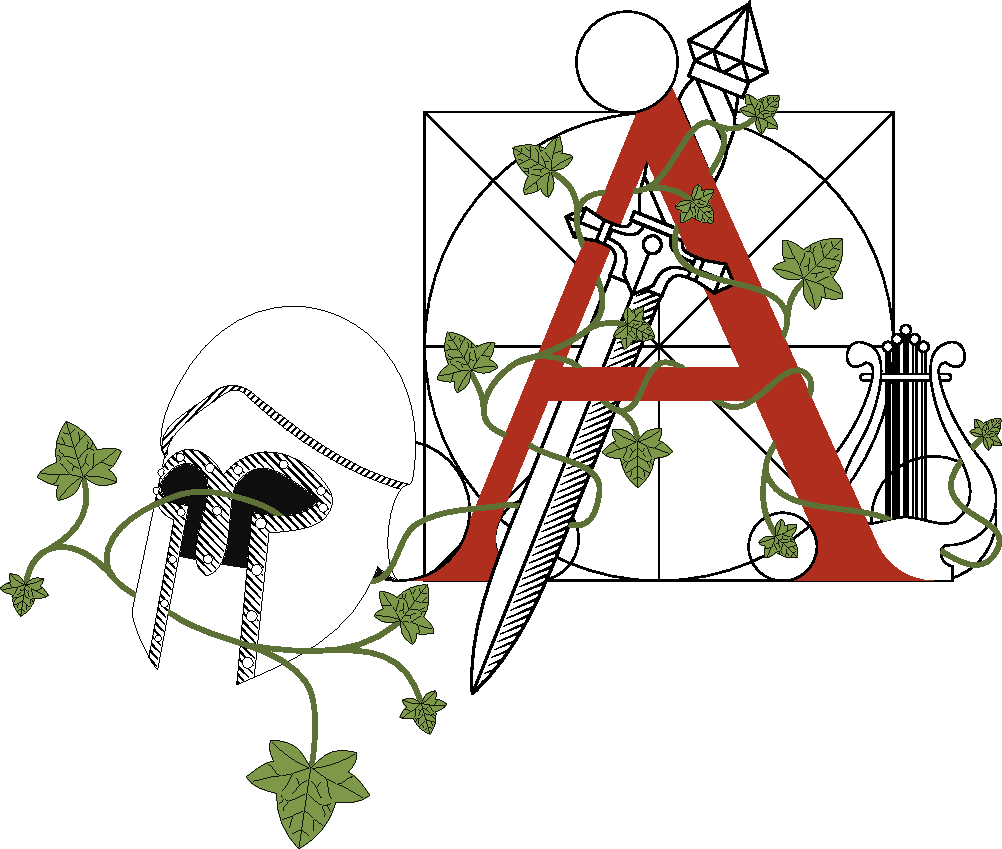
\includegraphics[width=0.36\textwidth]{lettrine-A-diborgo-grand.pdf}%
  }%
  \addcontentsline{lof}{figure}{Lettrine \autonym{A} aux divines proportions d’après l’alphabet de \textsc{di~Borgo} accompagné de lierre, lyre, casque corinthien, et dague}%
  \hspace{-0.2cm}{\color{rouge}\em\textsc{l’origine de ce diwan,}}
  oh oui, il y avait certes toute l’inspiration qui est y est à l’œuvre, de ces petits riens du quotidien que l’on ne sait précieux que lorsqu’on les perd. Instants fugaces si bien observés par Bashō\index{Artistes!Bashō} qui n’ont d’autre défauts que de nous en laisser insatiables comme l’a relevé Lissān~al\,Ḋḋīn, et ce parcequ’ils sont insaisissables. Or c’est malgré tout \incise{non pas en vain, espéré-je} qu’à travers la poésie je comptais en capter quelque instantané comme l’aurait fait \fallbackserif{Ȝ}omār Xayām ou sans doute même… Louis \textsc{Daguerre}\index{Photographie}.

  Or, ces infimes détails, présents de l’Éternel, s’ils sonnent comme un \xenism{carpe diem} c’est  que leur valeur ne s’acquière que parcequ’éphémères, et ils ne peuvent alors véritablement se jauger qu’à la faveur des deux principales activités de l’homme depuis la nuit des temps consacrant sa finitude au sein de sa grandeur que sont l’amour et la guerre. Pulsion de vie, pulsion de mort. Deux faces d’une même pièce, chacune variante de l’autre. Le titre de cet ouvrage aurait sans doute gagné à être donné en langue arabe où ces deux concepts se disent \xenism{ĥobb} \textarabic{حبّ} et \xenism{ĥarb} \textarabic{حرب} qui, fort prodigieusement ne varient que d’une seule lettre, révélant une assonance éloquente. Rappellerais-je à cet égard la parenté étymologique entre \xenism{bellum} (\enquote{guerre}) et \xenism{bellus} (\enquote{beau}) ⸮

   Il est même étrange que nombre de civilisations aient écarté les femmes de la guerre \incise{sauf, hélas, en tant que victimes}, alors qu’authentiquement elles auraient fait d’excellentes stratèges autant que de féroces combattantes. Pourtant, l’intuition des Grecs fit bien Aphrodite et Ares non seulement frère et sœur ainsi qu’amants mais encore frères de sang\index{Guerre!Sang} lorsqu’au chants \textsc{v} et \textsc{vi} de l’\work{Iliade} la même flèche du téméraire Diomède les blessa tous deux.

  L’amour est assurément une lutte, tandis que la guerre procède par la séduction. Sun Tzu ne dit-il pas si bien \enquote{Faîtes en sorte que vos prisonniers se retrouvent mieux chez vous qu’ils ne le seraient dans leur propre camp}, leçon dont s’instruirait fructueusement un amant ? La rime y répond.

  Il y avait tout cela, dis-je, au fondement de mes quelques vers. Mais en réalités, il n’aurait jamais été prit la peine de saisir le qalām\index{Ecriture@Écriture!Qalām}, le stylographe, le porte-plume, la bombe de peinture aérosol, ou le clavier\index{Ecriture@Écriture!Typographie}, s’il n’y avait pour transcender le tout, ma plus énamourée maitresse, celle qui me teint éveillé tant de nuits et pour qui le premier poème ne pouvait qu’être dédié.
}

\poemtitle{Complainte de l’insomniaque}\index{Café!Café personnifié en femme}\index{Insomnie}\index{Humour}
%\setIndexNameEntry[]{}
%\setIndexNameEntry[]{}
\begin{verse}\quatrain
  À mes nuits, elle est la plus fidèle amante\rhyme{ante}\\ \metric{11}
  Puisqu’à nos noces les témoins se sont assoupis.\rhyme{i}\\ \metric{13}
  Et si souvent, de ses charmes elle me tente,\\ \metric{12}
  C’est qu’elle se faufile et se love jusqu’à mon lit. \metric{14}

  Jalouse, elle évince une à une ses rivales,\rhyme{le}\\ \metric{12}
  Verveine, camomille, tisane, aucune ne l’accable.\\ \metric{15}
  Mais toi, café son acolyte, lui ouvre les volets\rhyme[e]{é}\\ \metric{15}
  À chaque fois qu’elle trouve porte fermée.  \metric{12}% 12
\end{verse}

\begin{prose}
  Car enfin, ne vous étonnez pas qu’au toucher, ce livre vous paraisse quelque peu humide, c’est qu’il est tout le long traversé d’une intarissable nappe de café.
\end{prose}

\begin{prose}
  D’ailleurs, c’est devant la porte d’un établissement-café où j’attendais quelqu’un que m’apparut le haïku suivant. Au dessus d’un recueil de Bashō\index{Artistes!Bashō} que je lisais, se trouvait une bouche d’égout.
\end{prose}

\poemtitle{De la bouche d’égout}\index{Urbanité}
\setIndexNameEntry[bouche d’égout]{De la bouche d’égout}
\begin{verse}\haiku
  La bouche d’égout,\rhyme{ou}\\  % H
  Les jambes de l’élégante\\  % H
  Y ont rendez-vous.
\end{verse}

\poemtitle{De la nappe de café}\index{Café}\index{Femmes!Cheveux}
\setIndexNameEntry[nappe de café]{De la nappe de café}
%\setIndexNameEntry[]{}
\begin{verse}\haiku
  Sur sillon dorsal,\\  % H
  Fuit la nappe de café.\\  % H
  Des cheveux châtain.
\end{verse}

\poemtitle{Du cheveu sur la manche}\index{Café}\index{Femmes!Cheveux}
\setIndexNameEntry[cheveu sur la manche]{Du cheveu sur la manche}
%\setIndexNameEntry[]{}
%\setIndexNameEntry[]{}
\begin{verse}\haiku
  Café à la main,\rhyme{ain}\\  % H
  Sur la manche de ma veste,\\  % H
  Un cheveu châtain.
\end{verse}

\begin{prose}
  C’est plus tard dans la soirée que les vers de Lissān~al\,Ḋḋīn ibn~al\,Xatīb\index{Al\,Andalous!Lissān~al\,Ḋḋīn ibn~al\,Xatīb} me vinrent à l’esprit pour s’accorder au moment.
  Ils étaient si à propos qu’il m’a semblé que de son \textsc{xiv}\ieme{} siècle il me les destinait.
  Ibn~Zamrak, toi qui instruisit son procès pour hérésie, que ne l’as-tu condamné, que ne l’as-tu exécuté et brulé ses restes  à la porte Calcinée de Fez, il n’empêche que ses cendres flottaient dans les airs ce soir là.
\end{prose}

\poemtitle{Flamme dans la nuit}
%\setIndexNameEntry[]{}
%\setIndexNameEntry[]{}
%\setIndexNameEntry[]{}
\begin{verse}\quatrain
  Ô nuit\index{Nuit}, drape de sombreur nos délits\rhyme{i}\index{Al\,Andalous}\\ \metric{10}
  Qui sous le voile noir cueillent un fruit.\\ \metric{10}
  Ô yeux%
  \endnote{Dans la poésie et la musique arabe, les mots apostrophés \autonym{ô nuit} (\textarabic{يا ليل}) et \autonym{ô yeux} (\textarabic{يا عين}), sont d’ordinaire utilisés comme vocalises.},\index{Femmes!Yeux}%
  \label{foot.vocaliseYeuxNuit} ne soyez  éblouis du feux\rhyme{eu}\\ \metric{10}
  Qui, ardent, trahi les amants pieux.\index{Amour} % 10
\end{verse}

\poemtitle{Mélancolie}
\setIndexNameEntry[Melancolie]{Mélancolie}
%\setIndexNameEntry[]{}
%\setIndexNameEntry[]{}
\begin{verse}\quatrain
  Les larmes que tu extirpas de mon âme\rhyme{ame}\\ \metric{11}
  Ne suffirent pas à calmer le brasier\rhyme[e]{é}\index{Feu}.\\ \metric{11}
  Et je noierais mon chagrin dans le café\index{Café}\index{Amour}\\ \metric{11}
  S’il n’avait apprit à y nager, l’infâme. % 11
\end{verse}

\poemtitle{Parole}
%\setIndexNameEntry[]{}
%\setIndexNameEntry[]{}
%\setIndexNameEntry[]{}
\begin{verse}\quatrain
  Un seul mot sucré d’elle\rhyme[ele]{èle}\index{Amour}\\ \metric{6}
  Vaut mieux que mille paroles.\rhyme{ol}\\ \metric{7}
  Il emprunte aux alvéoles\\ \metric{7}
  La gelée et le miel. % 6
\end{verse}

\poemtitle{Âme de cristal}
\setIndexNameEntry[ame de cristal]{Âme de cristal}
%\setIndexNameEntry[]{}
%\setIndexNameEntry[]{}
\begin{verse}\quatrain\sizain
  Ce sont des pleures fatales qu’elle pousse,\rhyme{ousse}\index{Femmes}\\ \metric{11}
  À chaque arpège d’Astor Piazzolla.\index{Artistes!Astor \textsc{Piazzola}}\rhyme{ola}\index{Musique}\\ \metric{11}
  Mais, sur ses joues, les perles qui s’éclaboussent,\\ \metric{11}
  Indélébiles, sont des larmes de verre\rhyme[ere]{ère}\\ \metric{11}
  Qui pleuvent pareilles au pianola\\ \metric{11}
  Aussi irrépressibles et régulières. % 11

  L’on ne peut les essuyer ni les briser\rhyme{rizé}\\ \metric{11}
  Mais leur point faible en est le \rhyme{amen}filament%
  \endnote{Allusion aux larmes de verre, artefact verrier dont le bulbe résiste à des chocs puissants tandis que le filament, s’il est rompu fait éclater l’ensemble.}\\ \metric{10}
  Qui, rompu, rend les plaies cicatrisées\\ \metric{10}
  Et les larmes étoiles du firmament.\index{Astronomie!Etoiles@Étoiles} % 11

  Mais que peuvent verser d’autre, ses yeux\index{Femmes!Yeux} ivrognes\rhyme{ogne}\\ \metric{12}
  Elle qui est une bouteille de Bologne%
\endnote{Ces bouteilles ont la particularité de résister à des coups de masse exercés depuis l’extérieur alors que le moindre objet en contact avec l’intérieur pulvérise toute la bouteille.},\\ \metric{12}
  Solide et imprenable de l’extérieur\rhyme[terieur]{térieur}\\ \metric{12}
  Mais pourtant vulnérable de l’intérieur ? % 12
\end{verse}

\poemtitle{Du cheveu d’airain}
\setIndexNameEntry[cheveu d’airain]{Du cheveu d’airain}
%\setIndexNameEntry[]{}
%\setIndexNameEntry[]{}
\begin{verse}\haikuII
  Des cheveux d’airain\rhyme{rain}\index{Femmes!Cheveux}\\  % H5
  Tombant sur les reins,\\  % H5
  Et je prends congé du monde. % H7
\end{verse}


\poemtitle{Le sentier pavé d’or}\index{Dune}\index{Destin}
\setIndexNameEntry[sentier pavé d’or]{Le sentier pavé d’or}
%\setIndexNameEntry[]{}
%\setIndexNameEntry[]{}
\begin{verse}\sizain
  Tous les rayons du soleil\index{Astronomie!Soleil} se recueillent\rhyme{ceuye}\\ \metric{10}
  Là où s’illumine un sûr corridor\rhyme{dor}\\ \metric{10}
  Jalonné d’accrocs, d’embûche et d’écueils.\\ \metric{10}
  Et c’est vêtu de haillons et pieds nus\rhyme{nu}\\ \metric{10}
  Que s’emprunte le sentier pavé d’or,\\ \metric{10}
  Le sentier glorieux qui mène aux nues.\index{Astronomie} % 10
\end{verse}

\poemtitle{Jardins d’Al\,Andalous}\index{Jardins}\index{Al\,Andalous!Alhambra}
%\setIndexNameEntry[]{}
%\setIndexNameEntry[]{}
\begin{verse}\quatrain\sizain
  Célébrée dans les vers de Lissān~al\,Ḋḋīn\index{Al\,Andalous!Lissān~al\,Ḋḋīn ibn~al\,Xatīb}%  %  1
  \endnote{Lissān~al\,Ḋḋīn écrivit le muwachaĥ \work{Jadaka al\,ṙaytu} faisant montre de nostalgie envers sa vie à Al\,Andalous.}\rhyme{ine}\\  % X
  Et portée par la voix de Juan {Martin}%
\endnote{Juan \textsc{Martin} interpréta le muwachaĥ andalous du \work{Lammā Bāda} dans son album \work{Musica Alhambra} parrut en 1998.},\index{Artistes!Juan \textsc{Martin}}\index{Musique}\\ \metric{11}
  Seuls l’oud\index{Musique!Oud} et le kanoun%
\endnote{De l’arabe \textarabic{قاﻧﻮﻥ}. Instrument à cordes pincées, de la famille des cithares sur table.}\index{Musique!Kanoun}\label{foot.kanoun} nous font parvenir\rhyme{venir}\\ \metric{11}
  L’apaisant clapotement de tes fontaines.\rhyme{taine}\index{Eau}\\ \metric{11}
  Al\,Andalous, si proche mais si lointaine,\\ \metric{11}
  Je souris encore à ton seul souvenir. % 11

  Qui des Almoravides aux Almohades,\rhyme{ade}\index{Histoire!Histoire arabo-musulmane}\\ \metric{11}
  Demeura fort belle jusqu’aux taïfas\rhyme{a}\\ \metric{11}
  Et l’est toujours malgré la Reconquista\index{Al\,Andalous!Reconquista}\\ \metric{11}
  Même si elle te porta l’estocade. % 11

  Car la prise de  Moussa Ibn Noçaïr\rhyme[e]{ère}\index{Personnages historiques!Moussa Ibn~Noçaïr}%
  \endnote{Wali et général du calife omeyade. Personnalité de premier plan dans la conquête d’Al\,Andalous.}\\ \metric{11}
  Est, à la poésie et l’architecture\rhyme{ture}\index{Architecture},\\ \metric{11}
  Non le berceau mais plus encore l’ovaire\\ \metric{11}
  D’où bourgeonneront bientôt mille cultures. % 11

  Et l’étoile\index{Astronomie!Etoiles@Étoiles} depuis trop longtemps éteinte\rhyme{einte}\index{Astronomie}\\ \metric{11}
  Qui est encore visible dans le ciel\rhyme{ciel}\\ \metric{11}
  Est semblable à tes beautés inertielles,\\ \metric{11}
  Celles dont nous parvient encore l’emprunte. % 11

  Plus que jamais prévaut le dit d’Alarcos\rhyme{cosse}%
  \endnote{La devise de l’émirat de Grenade qui fut par la suite reprise par les différentes entités politiques d’Al\,Andalous jusque sur leurs armoiries qui est \xenism{Wa la ṙāliba illa Allah.} (\enquote{Et il n’y a de vainqueur qu’Allah}) était frappée sur les bannières des armées musulmanes lors de la bataille d’Alarcos. D’ailleurs, les armoiries nasrides eurent ceci de singulier que, malgré les contacts intenses entre Arabo-musulmans et Européens, que ce soit à travers les croisades, la présence musulmane en Italie et en Sicile, ou l’invasion des territoires byzantins, aucune entité Arabo-musulmane ne jugea utile d’adopter la pratique occidentale de l’héraldique avant le XX\ieme{} siècle, à l’exception notable justement de l’émirat de Grenade. Lequel d’ailleurs ne fit qu’y faire figurer inlassablement son implacable devise.},\\ \metric{11}
  Funeste oracle digne de la Pythie\rhyme{ie}\index{Mythologie grecque}%
  \endnote{Pythie de Delphe dont l’oracle équivoque à Crésus lui annonçait qu’après la bataille qu’il devait mener, un grand empire allait s’effondrer. Après que Crésus ait mené sa bataille, un grand empire s’est effectivement effondré, le sien.}\\ \metric{11}
  Qui, gravé à l’envie sur les armoiries,\\ \metric{11}
  Rappelle ta disparition précoce\\ \metric{11}
  Car, partout jusqu’aux jardins de l’Alhambra\index{Al\,Andalous!Alhambra},\rhyme{a}\\ \metric{11}
Nous disons \xenism{Wa la ṙāliba illa Allah.} % 11
\end{verse}

\poemtitle{Un baiser}
\setIndexNameEntry[baiser]{Un baiser}
%\setIndexNameEntry[]{}
\begin{verse}\distique
  Ce n’était peut-être qu’un baiser\rhyme[e]{é}\index{Amour}\\ \metric{9}
  Mais il m’avait laissé bouche-bée. % 9
\end{verse}

\poemtitle{Portes d’Al\,Andalous}\index{Al\,Andalous}\index{Epique@Épique}
%\setIndexNameEntry[]{}
%\setIndexNameEntry[]{}
\begin{verse}\tercet%
  \rhyme{uss}
  Rapporte mes faits, Ibn~Tumulus% 9
  \endnote{Historien dont les chroniques sont le plus ancien témoignage sur la conquête d’Al\,Andalous nous étant parvenu.}.\\ \index{Personnages historiques!Moussa Ibn~Tumulus}\index{Histoire!Histoire arabo-musulmane} %
  Elle me promeut en général\rhyme{al}\\ \metric{9}
  Et fait couler les nefs dans mon dos.\index{Al\,Andalous!Tariq ibn~Zayad}% 9
  \endnote{Allusion au général Tariq ibn~Zayad. Personnage d’importance centrale dans la conquête d’Al\,Andalous au point qu’il donna son nom à Gibraltar (voulant dire montagne de Tariq). On raconte que suite à son débarquement en Hispanie, il craignit que ses soldats ne fuient devant le surnombre des Wisigoths si bien qu’il fit alors naufrager ses propres bateaux en annonçant à ses troupes \enquote{La mer est derrière vous et l’ennemi devant vous.}.}\rhyme{o}

  Rapporte sur de maints papyrus\index{Egypte@Égypte}\\ \metric{9}
  Que me suffit d’elle un seul sépale\\ \metric{9}
  Pour prendre l’Espagne aux Wisigoths.  % 9

  Rapporte et rappelle mordicus\\ \metric{9}
  Que lorsque son sourire s’étale\\ \metric{9}
  S’ouvrent les portes d’Al\,Andalous. % 9
\end{verse}

\begin{figure}[h]
  \centering
  
\includegraphics[height=3cm]{armoiries-grenade.pdf}
  \captionsetup{labelformat=empty}
  \caption[Armoiries nasrides de Grenade, d’après un relief de l’Alhambra, dont l’écu se blasonne ainsi \xenism{De gueule à la bande d’or, sur laquelle est écrit en arabe cursif \enquote{\textarabic{لا غالب إلا الله}} (\xenism{Il n’y a de vainqueur qu’Allah})}]{}
  \index{Al\,Andalous!Alhambra}
\end{figure}

\poemtitle{Artisan de l’Alhambra}\index{Al\,Andalous!Alhambra}\index{Architecture}
%\setIndexNameEntry[]{}
%\setIndexNameEntry[]{}
\begin{verse}\quatrain
  Es-tu chirurgien esthétique ou graveur\rhyme{veur}\\ \metric{12}
  Quand, du mur, ton bistouri ripa de sa lame\rhyme{lame}\\ \metric{12}
  Et fut poinçon sur mon visage de rêveur,\\ \metric{12}
  Pour y écrire l’ivresse tel un qalām\index{Ecriture@Écriture!Qalām} ? % 12

  Si les murs de l’Alhambra tu les fis fleurir\rhyme{rire}\index{Fleur},\\ \metric{12}
  Toi jardinier qui trace la calligraphie\rhyme{igraphie}\index{Ecriture@Écriture!Calligraphie},\\ \metric{12}
  C’est sur mes traits que ta florale épigraphie\\ \metric{12}
  S’est prolongée quand j’ai esquissé un sourire. % 12
\end{verse}

\poemtitle{De l’assise}\index{Humour}
\setIndexNameEntry[assise]{De l’assise}
%\setIndexNameEntry[]{}
\begin{verse}\haiku
  Quand elle s’assied\rhyme[e]{é}\index{Femmes}\\  % H
  Que ses  reins se sont creusés,\\  % H
  Une poire est née.
\end{verse}

\poemtitle{La nymphe}
\setIndexNameEntry[nymphe]{La nymphe}
%\setIndexNameEntry[]{}
\begin{verse}\sizain
  Même les hommes les plus intègres\rhyme[egre]{ègre}\index{Femmes}\\ \metric{9}
  Cèdent à sa silhouette allègre\\ \metric{9}
  Voulue par Dieu si belle, si belle\rhyme{ele}\\ \metric{9}
  Que s’élèvent au ciel des arpèges\rhyme[ege]{ège}\index{Musique},\\ \metric{9}
  Emportant loin les feuilles de liège,\\ \metric{9}
  Laissant en émoi la citadelle. % 9
\end{verse}

\begin{prose}
  Dans la nouvelle revue \enquote{Par ici la sortie}, M\textsuperscript{me}\,Margaret \textsc{Artwood}\index{Artistes!Margaret \textsc{Artwood}} nous parle d’une image iconique, sans doute même partagée par l’imaginaire de chacun, d’un chevalier\index{Chevaux} qui \enquote{galope à bride abattue vers un château dont le pont-levis se relève \textelp{} cavalier et monture décrivent alors un saut prodigieux afin de franchir les douves}. Sans doute qu’à l’heure des vacillements suscités par la pandémie et envers le péril du changement climatique, cette scène mobilise des espoirs et probablement même une métaphore de l’instant opportun à saisir par l’humanité, celui où plus que jamais il convient de fixer du regard le pont-levis plutôt que de regarder en arrière.

  Puisse alors de son \textsc{xi}\ieme{} siècle AÈC porter encore la voix de Pittacos de Mytilène\index{Philosophie grecque} qui disait déjà \enquote{Sache reconnaître le moment opportun} ; puisse-t-il se faire entendre de nous.

  Compte à M\textsuperscript{me}\,Margaret \textsc{Artwood} qui a voulu chercher cette scène que nous connaissons évidement tous, que nous avons certainement vu dans un film de chevalerie ou de cape et d’épée, elle nous apprend dans le \enquote{Time} que nous avons sans doute été victime d’un effet Mandella. Car elle n’a rien trouvé d’autre que des photos de voitures tombées dans un lac et un épisode de la panthère rose. Cette scène n’a jamais été filmée.
\end{prose}


\poemtitle{Kaïros — Le moment opportun}\index{Guerre!Chevalerie}\index{Destin}\index{Chevaux}\index{Epique@Épique}
\setIndexNameEntry[Kairos — Le moment opportun]{Kaïros — Le moment opportun}
%\setIndexNameEntry[]{}
\begin{verse}\quatrain
  Vous croyez que c’était un cavalier\rhyme[lie]{lié}\\ \metric{10}
  Mais c’est un vif éclair qui est passé.\rhyme[asse]{assé}\\ \metric{10}
  Homme et monture à tout jamais liés,\\ \metric{10}
  Ils vont au loin occire ou trépasser.  % 10

  Voilà un bref instant non écrit de l’histoire,\rhyme{toire}\\ \metric{12}
  De ces points de bascule où le cours peut changer\rhyme{gé}\\ \metric{12}
  Et emprunter une inattendue trajectoire.\\ \metric{12}
  Un moment que l’on ne peut saisir qu’enragé.  % 12

  Un chevalier qui galope à bride abattue\rhyme{batu}\\ \metric{12}
  Vers un château dont le pont-levis se relève,\rhyme[leve]{lève}\\ \metric{12}
  \incise{Tant qu’il n’est pas encore clôt nul n’est battu}\index{Destin}\\ \metric{12}
  Vers la muraille en approche, il saisit son glaive\index{Ecriture@Écriture!Epigraphie@Épigraphie}.  % 12

  Il n’y a qu’une infime chance, un interstice\rhyme{isse}\\ \metric{12}
  Mais saisit, il parachèvera la victoire.\rhyme{oir}\\ \metric{12}
  Tandis que les mètres restants sont un supplice,\\ \metric{12}
  Le pont qui s’élève encore peut toujours choir.  % 12

  Il n’en est rien, car il est déjà hissé haut.\rhyme{o}\\ \metric{12}
  Cavalier et monture sautent prompts sur l’eau\\ \metric{12}
  D’un saut prodigieux et franchissent les douves,\rhyme{ouve}\\ \metric{12}
  Rayonnants dans les cieux de leur regard de louve.

  Suspendus, leur élan est un instantané,\rhyme{tané}\\ \metric{12}
  Car la physique qui hésite et se flagelle,\rhyme[ele]{èle}\\ \metric{12}
  Entre la gravité et mouvement, chancelle\\ \metric{12}
  Et a tranché pour les deux en simultané.  % 12

  Dans leur ascension et leur chute si frêles\rhyme[iel]{ièl}\\ \metric{12}
  Ils ne sont nul part ailleurs qu’accrochés au ciel\\ \metric{12}
  Ni dans le faussé, ni les sabots au planché.\rhyme{ché}\\ \metric{12}
  Ils sont à cet endroit là à jamais perchés.  % 12
\end{verse}


\newpage{}
\thispagestyle{empty}
\AddToShipoutPictureFG*{%
  {
    \textnormal
    \AtPageLowerLeft{\input{img/oumayma.pdf_tex}}
    \setIndexNameEntry{Oumayma}
    \index{Femmes!Cheveux}%
    \haiku%
    \rhyme{lame}%
  }
}
~
\vfill
\pagebreak
%}


\section*{Casablanca}
\markboth{}{Casablanca}
\addcontentsline{toc}{section}{Casablanca}


\begin{prose}
  J’ai dû quitter tôt, trop tôt, mon agréable compagnie pour Casablanca où m’ont appelé certaines affaires. Ces affaires là n’étaient certes pas de la dernière urgence, mais comme j’ai toujours voulu caser quelque part cette phrase là qui donne l’impression d’être très occupé, eh bien j’ai trouvé que la situation y seyait bien ! Toujours est-il que si la ville est certes réputée sale et polluée, par chance j’arrivai un jour où le ciel clair m’inspira le haïku :
\end{prose}

\poemtitle{Du ciel bleu}\index{Urbanité}
\setIndexNameEntry[ciel bleu]{Du ciel bleu}
%\setIndexNameEntry[]{}
\begin{verse}\haiku
  D’entre les immeubles,\\  % H
  Jaillit une vérité,\\  % H
  Celle du ciel bleu.
\end{verse}

\begin{figure}[h]
  \centering
  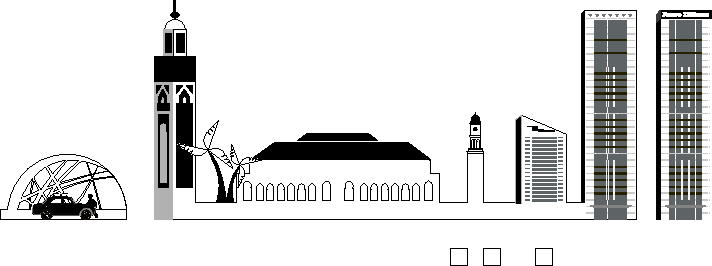
\includegraphics[width=\textwidth]{casablanca-alone.pdf}
  \captionsetup{labelformat=empty}
  \caption[Idéotexte de \autonym{Casablanca} (\textarabic{البيضاء})]{}
  \index{Urbanité}
\end{figure}

\poemtitle{Baiser ensoleillé}\index{Astronomie!Soleil}
%\setIndexNameEntry[]{}
%\setIndexNameEntry[]{}
\begin{verse}\sizain
  Ayant sur l’horizon surfé,\rhyme{fé}\index{Astronomie}\\ \metric{8}
  Nos embrassades crépusculaires\rhyme[ere]{ère}\index{Amour}\\ \metric{9}
  Trempèrent  le soleil dans la mer\\ \metric{9}
  Tel un \xenism{cookie} dans le café\\ \metric{8}
  Si bien que des palmiers et néons\rhyme{néon}\index{Synthwave}\\ \metric{9}
  Ses lèvres m’ont laissé que néant.\index{Femmes}  % 9
\end{verse}

\poemtitle{Le déphasé}
\setIndexNameEntry[dephasé]{Le déphasé}
%\setIndexNameEntry[]{}
\begin{verse}\quatrain
  Quelque part entre le néant et l’infini,\rhyme{ni}\\ \metric{12}
  Enivré d’amour\index{Amour} et d’insomnie\index{Insomnie},\\ \metric{9}
  Je me perdis en leur compagnie\\ \metric{9}
  Ne sachant dire s’il est midi ou minuit.\rhyme{i}  % 12

  Chauve-souris dans une chambre anéchoïque\rhyme{ic}\\ \metric{12}
  Que je suis, parmi les néons en mosaïque\index{Synthwave}\\ \metric{12}
  Lorsque je somnambule de nuit dans la rue\rhyme{u}\index{Urbanité},\\ \metric{12}
  Perdu dans des endroits qui me sont bien connus.  % 12
\end{verse}

\poemtitle{À l’écoute}
\setIndexNameEntry[a lecoute]{À l’écoute}
%\setIndexNameEntry[]{}
\begin{verse}\quatrain
  À trop écouter mes désirs\rhyme{sir}\\ \metric{8}
  J’en suis devenu sourd\rhyme{our}\\ \metric{6}
  Et ma raison s’en vit gésir\\ \metric{8}
  Pourfendue par l’amour.\index{Amour}  % 6
\end{verse}

\poemtitle{La ville catin}
\setIndexNameEntry[ville catin]{La ville catin}
%\setIndexNameEntry[]{}
\begin{verse}\quatrain
  Casablanca, aussi belle que tes catins\rhyme{ain}\index{Urbanité}\\ \metric{12}
  Qui, quoique distinctes, racolent en ton sein.\\ \metric{12}
  Dégoûtante comme celles des bas cartiers,\rhyme{tier}\\ \metric{12}
  Princière comme les escortes de Gauthier% 12
  \endnote{Cartier réputé bourgeois de Casablanca.}.
\end{verse}

\begin{prose}
  Il y a bien là force disgrâce et grande hideur mais elle est moins du fait des braves personnes de la classe laborieuse, celles que quelques esprits aigris et médisants sont prompts à vilipender.

  C’est dans un cartier de privilégiés, aux gens débordants d’une suffisance qui, à la vérité me fit esclaffer davantage qu’elle ne m’indisposa, que m’apparut la mocheté. Celle-ci n’aurait pu être pour moi que motif de brocard et ne pas susciter outre mesure de réflexion, si elle ne manqua d’être grave.
\end{prose}

\poemtitle{La lutte des places}
\setIndexNameEntry[lutte des places]{La lutte des places}
%\setIndexNameEntry[]{}
\begin{verse}\quatrain
  On dit que les bourgeois sont méritants,\rhyme{an}\\ \metric{10}
  Que leurs risques valent leurs privilèges,\rhyme{ilège}\\ \metric{10}
  Que de leurs exploits on fait florilège.\\ \metric{10}
  Rien n’est plus faux, voyons-le sur le champs.  % 10

  Je traverse le passage piéton\rhyme{an}\\ \metric{10}
  Quand un bourgeois de soixante-dix ans,\\ \metric{10}
  Plein d’insolence et de désinvolture,\rhyme{ture}\\ \metric{10}
  Prétend forcer le passage en voiture.  % 10

  Je l’aperçois me charger le vieillot,\rhyme{o}\\ \metric{10}
  Dans son armure de fer, tout penaud.\\ \metric{10}
  Je le vois, il fonce, je continue.\rhyme{nu}\\ \metric{10}
  Alors il freine sec sur l’avenue.

  Bon bah, désolé vieux ça va pas l’faire.\rhyme{fer}\\ \metric{10}
  Si puissant dans ton armure de fer.\\ \metric{10}
  Tu t’es arrêté, tout grand manitou,\rhyme{ou}\\ \metric{10}
  À vingt centimètre de mon genoux.  % 10

  Et bien que fautif, il klaxonne, mécontent.\rhyme{en}\\ \metric{12}
  Je vais à sa fenêtre traiter avec lui,\rhyme{ui}\\ \metric{12}
  Lui, montrer son tort, résoudre le différent.\\ \metric{12}
  Mais alors ne voilà-t-il donc pas qu’il s’enfuit !  % 12

  Je reconnais là leur légendaire valeur\rhyme{eur}\\ \metric{12}
  Qui justifie hauts salaires en si peu d’heures.\\ \metric{12}
  Il y a là du mérite et tant de civisme\rhyme{ivizme}\\ \metric{12}
  Qu’il ne s’agit assurément pas d’arrivisme.  % 12

  Ayant agis ainsi avec un prolétaire,\rhyme[tere]{tère}\\ \metric{12}
  Je m’en souviens, un ouvrier de caractère.\\ \metric{12}
  Il est vrais qu’il était tout aussi effronté\rhyme{fronté}\\ \metric{12}
  Mais voilà, il était resté pour m’affronter.  % 12
\end{verse}

\begin{prose}
%  Il se trouve qu’ayant lu ce poème, un ami me fit remarquer qu’à mon intuition poétique existe des fondements scientifiques, puisqu’une publication\endnote{\cite{Piff4086}} de l’université du Michigan corroborer la propension à l’arrogance des personnes à haut revenus à adopter des comportements manquant d’étiques.

  Mystère de l’intuition poétique qui s’étaye de fondements scientifiques ; il se trouve que peu de temps après avoir vécu cet épisode et rédigé le poème qui en parle, une publication\endnote{\cite{Piff4086}} de l’université du Michigan corrobora l’arrogance des personnes à hauts revenus et leur propension à adopter des comportements manquants d’étiques et mortellement dangereux.

  Est-ce sans doute que certains signaux faibles, des indices subreptices ne se révèlent qu’à la faveur des  sentiments du poète alliés aux instruments du scientifique.
\end{prose}

\poemtitle{Immigration}\index{Epique@Épique}
%\setIndexNameEntry[]{}
%\setIndexNameEntry[]{}
\begin{verse}\tercet
  Tracez puissantes nefs\index{Mer!Navigation}\\ \rhyme[efe]{èfe}\metric{6}
  Des sillons sur les sept mers\\ \rhyme[ere]{ère}\metric{7}
  Qui mènent aux champs verts.  % 6

  Oui, tracez derechef\\ \metric{6}
  Loin vers les terres  nouvelles\\ \rhyme[ele]{èle}\metric{7}
  Léguées par l’Éternel  % 6

  Où s’écrira l’aleph\index{Ecriture@Écriture!Calligraphie}.\\ \metric{6}
  Tel le qalām\index{Ecriture@Écriture!Qalām} qui écarte\\ \rhyme{carte}\metric{7}
  Les ondes sur la carte  % 6

  Formant un nouveau fief\\ \metric{6}
  Qu’investi le peuple entier\\ \rhyme{tié}\metric{7}
  Pour bâtir des chantiers  % 6

  Élevant aux reliefs,\\ \metric{6}
  Des mosquées, ou synagogues,\\ \rhyme{ogue}\metric{7}
  Églises où qu’il vogue.  % 6
\end{verse}

\poemtitle{Berserker}\index{Guerre}
%\setIndexNameEntry[]{}
%\setIndexNameEntry[]{}
\begin{verse}\distique
  \textarm{When.I.break.my.gear,}%  5
  \endnote{Distique anglophone transcrit en runique pouvant se retranscrire en alphabet latin comme suit :

    \begin{longtable}[l]{ @{\hspace*{\parindent}} ll}
      When I break my gear, & \emph{Quand je brise mon écu,}\\
      I can lose my fear. & \emph{La peur me quitte.}  % 
    \end{longtable}}\\  \rhyme{ir}\metric{5}
  \textarm{I.can.lose.my.fear}\metric{6}  %  6
\end{verse}

\poemtitle[Kanoun d’Al\,Andalous]{Kanoun\endnotemark[\getrefnumber{foot.kanoun}] d’Al\,Andalous}%
%\setIndexNameEntry[]{}
\setIndexNameEntry{Kanoun d’Al\,Andalous}
%\renewcommand\currentpoemtitle{Kanoun d’Al\,Andalous}%
\index{Al\,Andalous}\index{Musique!Kanoun}
\begin{verse}\sizain
  Telle une femme fière qui ne se dompte\index{Femmes}\\ \rhyme[ante]{[a\textbar{}o]nte}\metric{11}
  Dont on longe de Cadix à Alicante,\\ \metric{11}
  Les imprenables formes et les côtes\index{Mer!Navigation},\\ \rhyme{cote}\metric{10}
  Al\,Andalous demeure un merveilleux conte.\\ \metric{11}
  Et morcelée en taïfas aliquantes\index{Histoire!Histoire arabo-musulmane},\\ \metric{11}
  Ses harmoniques restent aliquotes\index{Musique}.  % 10
\end{verse}

\poemtitle{Du sable mouillé}\index{Mer}
\setIndexNameEntry[sable mouillé]{Du sable mouillé}
%\setIndexNameEntry[]{}
\begin{verse}\haikuII
  Marchant sur la plage\\  % H5
  Au sable mouillé,\\  % H5
  Les vagues frôlent mes pieds.  % H7
\end{verse}

\poemtitle{Opérateur de marché}
\setIndexNameEntry[Operateur de marché]{Opérateur de marché}
%\setIndexNameEntry[]{}
\begin{verse}\quatrain
  Quand avec mon OPA je passe à l’attaque,\\ \rhyme{ac}\metric{12}
  Alors en Leica, en Nikon ou en Kodak\index{Photographie}\\ \metric{12}
  Les flashs rebondissent sur mes vitres opaques,\\ \metric{12}
  Tandis que mon indice est premier au NASDAQ.  % 12
\end{verse}

\poemtitle{De l’espoire du ressac}\index{Mer}\index{Destin}
\setIndexNameEntry[espoire du ressac]{De l’espoire du ressac}
%\setIndexNameEntry[]{}
\begin{verse}\haiku
  Devant l’océan,\\  % H
  Du son du ressac des vagues,\\  % H
  S’entend un espoir.
\end{verse}

\begin{prose}
  Mais si la beauté providentielle des choses de la nature comme le ciel et les arbres m’émut, je ne manquai pas d’être assailli par les laideurs bien humaines, tant les hommes y rivalisent de vices et de vanités. 

  Leur air grave de gens trop occupés semble dire qu’ils s’adonnent à je ne sais quelles choses bien grandiloquentes. Voyez-vous, la face un rien grimaçante qui laisse entendre combien leurs responsabilités sont cruciales au sein des services de renseignement ou qu’ils sont préoccupés par des choses de premier ordre\,; et ce alors qu’ils essayent une petite laine dans un commerce de vêtements. À en croire leur dégaine cérémonieuse, il s’agirait dans leur façon de se pavaner, de rien de moins que d’épopées homériques… ou de la \work{Comédie} d’Aristophane. %Il y avait grande dissonance entre les manières obséquieuses et la banalité de la situation que j’avoue m’être surpris à sourire ! Car si ce n’était ni les \work{Iliade} et \work{Odyssée} d’Homère, il ne pouvait s’agir là que de la \work{Comédie} d’Aristophane, vous dis-je. De quoi inspirer des hymnes au grotesque.
\end{prose}

\poemtitle{Odyssée consumériste}\index{Humour}
%\setIndexNameEntry[]{}
%\setIndexNameEntry[]{}
\begin{verse}\distique
  Ô Ulysse, pourquoi avais-tu quitté ton Ithaque,\\ \rhyme{ac}\metric{14}
  Si ce n’est pour apporter à ton fils télé et mac% 14
  \endnote{Kakemphaton avec \autonym{Télémaque}, fils d’Ulysse.} ?
\end{verse}

\poemtitle{Fratricide}
%\setIndexNameEntry[]{}
%\setIndexNameEntry[]{}
\begin{verse}\quatrain
  À la septième arche, Étéocle et Polynice,\index{Guerre}\index{Mythologie grecque}\\ \metric{12}\rhyme{isse}
  Vous qui d’Œdipe de Thèbes êtes les fils,\\ \metric{12}
  Vous n’hériterez de la terre de vos pères\\ \rhyme[ere]{ère}\metric{12}
  Que la largeur de la tombe où l’on vous enterre.  % 12
\end{verse}

\poemtitle{De la mosquée volante}
\setIndexNameEntry[mosquee volante]{De la mosquée volante}
%\setIndexNameEntry[]{}
\begin{verse}\haiku
  Dessus du houpier,\index{Architecture}\index{Islam}\\  \rhyme[ie]{ié}% H
  Flotte le grand minaret,\\  % H
  Et rien en dessous.
\end{verse}

\poemtitle{De la danse des algues}\index{Mer}
\setIndexNameEntry[danse des algues]{De la danse des algues}
%\setIndexNameEntry[]{}
\begin{verse}\haiku
  Sous l’eau crystaline,\\  % H
  Les algues tendent leurs bras\\  % H
  Et dansent pour moi.
\end{verse}

\begin{floatpoem}
  \poemtitle{Le chien}%
  \setIndexNameEntry[chien]{Le chien}%
  \calligramme
  \vspace{-1cm}
  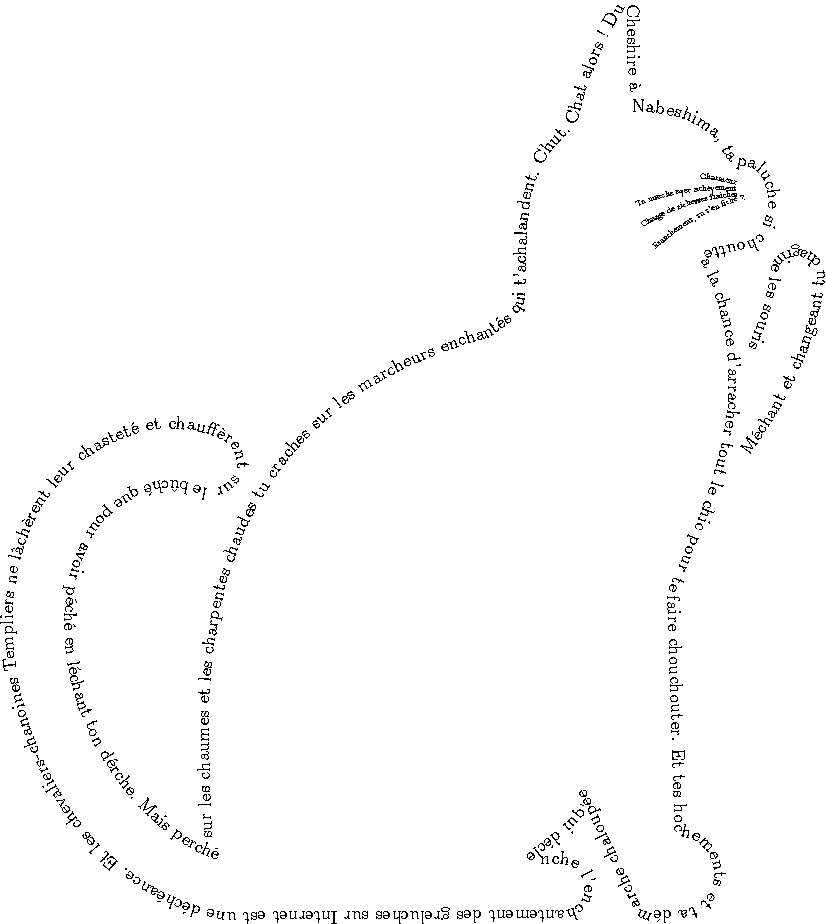
\includegraphics[width=\textwidth]{calligrame-chien.pdf}
\end{floatpoem}

\poemtitle{De la digue}\index{Mer}
\setIndexNameEntry[digue]{De la digue}
%\setIndexNameEntry[]{}
\begin{verse}\haiku
  Le ressac des vagues\\  % H
  Creuse la digue concave,\\  % H
  Et force sa courbe.
\end{verse}

\poemtitle{Du bruit du billard}
\setIndexNameEntry[bruit du billard]{Du bruit du billard}
%\setIndexNameEntry[]{}
\begin{verse}\haiku
  Flamme tamisée.\index{Synthwave}\\  % H
  Quand je rentre dans un bar,\\  \rhyme{ar}% H
  J’entends le billard.
\end{verse}



\begin{prose}
  Je passais du reste de nombreuses heures sur les terrasses des cafés où les rayons du soleil\index{Astronomie!Soleil} m’apportaient d’inspirantes pensées.
\end{prose}

\poemtitle[Ivresse à Kaffa]{Ivresse à Kaffa\endnote{Le titre du quatrain est dû au fait que la culture et la boisson du café vit le jour à Kaffa, en Éthiopie.}}%
\setIndexNameEntry{Ivresse à Kaffa}
%\setIndexNameEntry[]{}
%\renewcommand\currentpoemtitle{Ivresse à Kaffa}%
\index{Café}\index{Propos réflexif}
\begin{verse}\quatrain
  Xayām% 9
  \endnote{L’apostrophe de Xayām, poète bachique iranien, lui rappelle son erreur et instaure une rivalité entre vin et café.},\index{Artistes!Omar Xayam@\fallbackserif{Ȝ}omār Xayām}\label{foot.xayam} il y a grande méprise.\\  \rhyme{prise}% X
  Fille de la vigne que tu prises\\ \metric{9}
  N’est exquise face au chaud ou froid\index{Café!Rivalité Café-Alcool}\\ \metric{9}
  Café qui excite notre émois.  % 9
\end{verse}

\poemtitle{Fortune, impératrice du monde}\index{Destin}\index{Epique@Épique}
%\setIndexNameEntry[]{}
%\setIndexNameEntry[]{}
\begin{verse}\quatrain
  Que savons-nous du dernier Abencérage% 11
\endnote{Famille puissante d’Al\,Andalous.}\label{foot.Abencerage}\index{Al\,Andalous!Abencérage} ?\\  \rhyme{rage}%
  Naguère son clan essaima dans Grenade,\\ \rhyme{ade}\metric{11}
  Aujourd’hui, de leur fières fanfaronnades,\\ \metric{11}
  L’on ne retint plus rien, sinon un mirage.  % 11

  Eux qui se pensaient plus puissants que l’émir,\\ \rhyme{ire}\metric{11}
  Au point de vouloir régner sur tous les Maures,\\ \rhyme{mor}\metric{11}
  Ne purent bâtir leur insolent empire\\ \metric{11}
  Nul part ailleurs que dans la sublime mort.  % 11

  Même le trône qu’ils croient édifier,\\ \rhyme[e]{é}\metric{11}
  Pour voir que d’autres qu’eux y vont siéger,\\ \metric{11}
  Ne les y aura établis que Fortune,\\ \rhyme{ortune}\metric{11}
  Elle qui depuis toujours nous importune.  % 11
\end{verse}

\poemtitle{Du charme de la nuit}\index{Nuit}
\setIndexNameEntry[charme de la nuit]{Du charme de la nuit}
%\setIndexNameEntry[]{}
\begin{verse}\haiku
  Que j’aime la nuit\\  \rhyme{i}% H
  Car tous les chats y sont gris\\  % H
  Et la ville aussi.\index{Urbanité}
\end{verse}

\poemtitle{Le marathonien}\index{Epique@Épique}
\setIndexNameEntry[marathonien]{Le marathonien}
%\setIndexNameEntry[]{}
\begin{verse}\quatrain
  Cours et la douleur s’en ira\\ \rhyme{ra}\metric{8}
  Par la fermeté et l’effort.\\ \rhyme{or}\metric{8}
  Cours, la douleur disparaîtra\\ \metric{8}
  Et avec elle tous les torts.  % 8

  Jusqu’au suintement de sueur\\ \rhyme{eur}\metric{8}
  Sur ton arcade sourcilière,\\ \rhyme[iere]{ière}\metric{8}
  Tu courras de toute fureur.\\ \metric{8}
  Tu courras le visage fière.  % 8

  Cours, vas vers d’autres continents,\\ \rhyme{inan}\metric{8}
  Vers la mer où tu mets les voiles,\\ \rhyme{oile}\metric{8}
  Les pôles, les points culminants.\\ \metric{8}
  Cours vers le ciel, vers les étoiles.\index{Astronomie!Etoiles@Étoiles}  % 8
\end{verse}

\poemtitle{L’allier solaire}\index{Astronomie!Soleil}
\setIndexNameEntry[allier solaire]{L’allier solaire}
%\setIndexNameEntry[]{}
\begin{verse}\quatrain
  Je te prierai, à Dieu ne plaise, Aton% 
  \endnote{Aton était dans la mythologie égyptienne le dieu disque solaire souvent représenté avec des rayons qui en émanent.}\metric{11}\\ \rhyme{on}
  Pour poursuivre ta course dont les rayons,\\ \metric{11}
  Frappent tout droit et indisposent la belle\index{Femmes}\\ \rhyme[ele]{èle}\metric{11}
  Contrainte à des postures si criminelles.  % 11

  Pour s’y soustraire un peu et se mettre à l’ombre,\\ \rhyme{ombre}\metric{11}
  Elle recule, se tapit, et se cambre.\\ \metric{11}
  Mais le long de sa hanche jusqu’à sa croupe,\\ \rhyme{oupe}\metric{11}
  Se trace une courbe d’inédite coupe.  % 11
\end{verse}

\poemtitle{L’astronaute}\index{Astronomie}\index{Technique}\index{Destin}
\setIndexNameEntry[astronaute]{L’astronaute}
%\setIndexNameEntry[]{}
\begin{verse}\quatrain\sizain
  Ô, opérateur spatial, guide-moi.\\ \rhyme{oi}\metric{11}
  Aide mon astronef à se diriger.\\ \rhyme{jé}\metric{11}
  Qu’à travers l’espace où je vais voyager,\\ \metric{11}
  Je puisse trouver assurément la voie.\\ \metric{11}
  La voie pour tisser dans le ciel ma toile\\ \rhyme{toile}\metric{10}
  Entre les planètes et les étoiles.\index{Astronomie!Etoiles@Étoiles}  % 10

  Opérateur, lorsque je flotte en l’air,\\ \rhyme[ere]{ère}\metric{10}
  Déploie le canadarm%
  \endnote{Le bras canadien est un bras articulé mécanique conçu par le système industriel canadien et équipant certains engins spatiaux.} pour me saisir\\  %  10
  Dans ma sortie extra-véhiculaire\\  %  10
  Où j’observe les objets nébulaires.  %  10

  Opérateur, que tes instructions\\  \rhyme{tion}%  10
  Soient toutes gravées en hiéroglyphes\index{Ecriture@Écriture!Hiéroglyphes},\\  \rhyme{ife}%  10
  Lorsqu’aux commandes je suis émotif,\\  %  10
  Lorsque je déclenche l’ignition\index{Feu}.  %  10

  Opérateur, suivant tes conseils adroits,\\ \rhyme{droi}\metric{11}
  Tel la flèche d’un archer qui file droit\index{Archerie}\\ \metric{11}
  Et atteint sa cible avant d’être lâchée,\\ \rhyme{ché}\metric{11}
  Sur Mars où je m’en vais, j’ai déjà marché.  % 11
\end{verse}


\poemtitle{De la scie circulaire}
\setIndexNameEntry[scie circulaire]{De la scie circulaire}
%\setIndexNameEntry[]{}
\begin{verse}\haiku
  La scie circulaire\\  % H
  Agace en laps si stressant.\\  % H
  Et son son occis.
\end{verse}

\poemtitle{L’indice}
\setIndexNameEntry[indice]{L’indice}
%\setIndexNameEntry[]{}
\begin{verse}\distique
  Les yeux\index{Femmes!Yeux} des adolescentes disent\index{Femmes}\\ \rhyme{zen}\metric{9}
  Ce que les bouches des femmes taisent.  % 9
\end{verse}

\poemtitle{Filles de l’arc en ciel}\index{Femmes}\index{Astronomie}
%\setIndexNameEntry[]{}
%\setIndexNameEntry[]{}
\begin{verse}\quatrain\septain
  Ayant trouvé la cachette du leprechaun%
  \index{Mythologie}\endnote{Personnage du folklore celtique dont la cachette se trouve à l’endroit où \enquote{l’arc-en-ciel touche terre}.},\\ \rhyme{one}\metric{12}  % X
  J’ai posé mon guéridon près de l’arc-en-ciel\\ \rhyme[ele]{èle}\metric{12}
  Où j’ai goulûment puisé ma tasse atone\index{Café!Café personnifié en femme}\\ \metric{11}
  Que je ressorti pleine de jouvencelles.\metric{11}  % 

  Et les Pharisiens dont provient le blâme\index{Talmud}\\ \rhyme{ame}\metric{11}
  Qui, mord à la bouche et œillères aux tempes,\\ \rhyme[ampe]{[a\textbar{}e]mpe}\metric{11}
  Font saigner les murs de la ville%
  \endnote{Vue talmudique des Pharisiens qui, zélés dans leur expression de la pudeur, ferment les yeux ou se les cachent pour éviter de regarder les femmes. Au points qu’ils se cognent contre les murs et y saignent, selon la raillerie dont il font l’objet.}, se trompent\\  \metric{11}
  À tant détourner leurs yeux des jolies femmes\\ \metric{11}
  Et, d’entre les couleurs de deux belles âmes,\\ \metric{11}
  Préférer la bande noire d’Alexandre%11
  \endnote{Dans le phénomène râre du double arc-en-ciel, une bande sombre entre les deux apparait, appelée d’après son découvreur \autonym{bande d’Alexandre}.}\\ \rhyme[andre]{[a\textbar{}e]ndre} % X
  Seule dont ils soient à même de s'éprendre.  % 11
\end{verse}

%\begin{floatpoem}
  \poemtitle{Paradoxe de la ville}\index{Urbanité}\index{Architecture}\calligramme
  \begin{adjustwidth}{-1.2cm}{-2.5cm}% left
  %\begin{adjustwidth}{-0.3cm}{-3.5cm}% right
    {%\tiny%
    \scriptsize%
    \setstackTAB{&}%
    \fixTABwidth{E}%
    \tabbedCenterstack{
~&~&~&~&~&~&~&~&~&~&~&~&~&~&~&~&~&~&~&~&~&~&~&~&~&~&~&~&~&~&~&~&~&~&~&Â&M&E&~&~&~&~&~&~&~&~&~&~&~&~&~&~&~&~&~&~&~&~&~&~&~&~&~&~&~&~&~&~&~&\\
~&~&~&~&~&~&~&~&~&~&~&~&~&~&~&~&~&~&~&~&~&~&~&~&~&~&~&~&~&~&~&~&~&~&É&G&A&L&E&~&~&~&~&~&~&~&~&~&~&~&~&~&~&~&~&~&~&~&~&~&~&~&~&~&~&~&~&~&~&\\
~&~&~&~&~&~&~&~&~&~&~&~&~&~&~&~&~&~&~&~&~&~&~&~&~&~&~&~&~&~&~&~&~&~&B&E&L&L&E&~&~&~&~&~&~&~&~&~&~&~&~&~&~&~&~&~&~&~&~&~&~&~&~&~&~&~&~&~&~&\\
~&~&~&~&~&~&~&~&~&~&~&~&~&~&~&~&~&~&~&~&~&~&~&~&~&~&~&~&~&~&~&~&~&~&P&I&É&T&É&~&~&~&~&~&~&~&~&~&~&~&~&~&~&~&~&~&~&~&~&~&~&~&~&~&~&~&~&~&~&\\
B&L&A&N&C&H&E\rlap{,}&~&~&~&A&B&U&S&I&V&E\rlap{,}&~&~&~&~&~&~&~&~&~&~&~&~&~&~&~&~&~&V&R&A&I&S&~&~&~&~&~&~&~&~&~&~&~&~&~&~&~&~&~&~&~&~&~&~&~&~&~&~&~&~&~&~&\\
O&U&Ï&S&·&J&E\rlap{.}&~&~&~&F&É&L&O&N&N&E\rlap{,}&~&~&~&~&~&~&~&~&~&~&~&~&~&~&~&~&~&S&A&I&N&T&~&~&~&~&~&~&~&~&~&~&~&~&~&~&~&~&~&~&~&~&~&~&~&~&~&~&~&~&~&~&\\
T&O&N&·&N&O&M&~&~&~&E&T&·&D&R&U&E&~&~&~&~&~&~&~&~&~&~&~&~&~&~&~&~&~&D&É&V&O&T&~&~&~&~&~&~&~&~&~&~&~&~&~&~&~&~&~&~&~&~&~&~&~&~&~&~&~&~&~&~&\\
O&N&C&Q&U&E&S&~&~&~&M&A&I&S&·&S&I&~&~&~&~&~&~&~&~&~&~&~&~&~&~&~&~&~&A&M&È&N&E&~&~&~&~&~&~&~&~&~&~&~&~&~&~&~&~&~&~&~&~&~&~&~&~&~&~&~&~&~&~&\\
A&D&É&Q&U&A&T&~&~&~&G&É&N&I&A&L&E\rlap{.}&~&~&~&~&~&~&~&~&~&~&~&~&~&~&~&~&~&D&R&O&I&T&~&~&~&~&~&~&~&~&~&~&~&~&~&~&~&~&~&~&~&~&~&~&~&~&~&~&~&~&~&~&\\
É&G&A&R&E&R&A&~&~&~&T&O&I&,&·&T&U&~&~&~&~&~&~&~&~&~&~&~&~&~&~&~&~&~&B&R&A&V&E&~&~&~&~&~&~&~&~&~&~&~&~&~&~&~&~&~&~&~&~&~&~&~&~&~&~&~&~&~&~&\\
P&L&U&S&·&D&E&~&~&~&E&S&·&L&’&A&S&~&~&~&~&~&~&~&~&~&~&~&~&~&~&~&~&~&L&O&U&E&R&~&~&~&~&~&~&~&~&~&~&~&~&~&~&~&~&~&~&~&~&~&~&~&~&~&~&~&~&~&~&\\
M&A&U&V&A&I&S&~&~&~&D&E&·&C&Œ&U&R\rlap{,}&~&~&~&~&~&~&~&~&~&~&~&~&~&~&~&~&~&T&O&U&T&E&~&~&~&~&~&~&~&~&~&~&~&~&~&~&~&~&~&~&~&~&~&~&~&~&~&~&~&~&~&~&\\
D&I&A&B&L&E&S&~&~&~&L&A&·&D&A&M&E&~&~&~&~&~&~&~&~&~&~&~&~&~&~&~&~&~&B&O&N&T&É&~&~&~&~&~&~&~&~&~&~&~&~&~&~&~&~&~&Ô&~&~&~&~&~&~&~&~&~&~&~&~&\\
Q&U&E&·&L&E&S&~&~&~&D&E&·&B&O&U&E&~&~&~&~&~&~&~&~&~&~&~&~&~&~&~&~&~&P&I&T&I&É&~&~&~&~&~&~&~&~&~&~&~&~&~&~&~&~&~&V&I&L&E&~&~&~&~&~&~&~&~&~&\\
F&A&U&S&S&E&S&~&~&~&J&O&N&C&H&É&E&~&~&~&~&~&~&~&~&~&~&~&~&~&~&~&~&~&F&O&R&C&E&~&~&~&~&~&~&~&~&~&~&~&~&~&~&~&~&~&D&E&S&·&V&I&L&L&E&S\rlap{,}&~&~&~&\\
R&U&M&E&U&R&S&~&~&~&D&’&É&T&R&O&N\rlap{,}&~&~&~&~&~&~&A&U&X&·&M&O&T&S&·&D&’&A&M&É&N&I&T&É&·&E&T&·&B&O&N&T&É\rlap{,}&~&~&~&~&~&~&J&E&·&M&’&A&D&R&E&S&S&E&~&\\
D&E&·&T&O&U&T&~&~&~&M&I&A&S&M&E&S\rlap{,}&~&~&~&~&~&A&V&E&C&·&Q&U&E&L&Q&U&E&S&·&M&A&L&I&N&S&·&P&R&O&C&É&D&É&S&~&~&~&~&~&À&~&T&O&I&~&I&M&P&U&R&E\rlap{.}&~&\\
E&N&D&R&O&I&T\rlap{.}&~&~&~&O&R&D&U&R&E&S\rlap{,}&~&~&~&~&~&T&U&·&L&E&U&R&·&O&P&P&O&S&E&·&T&E&S&·&D&I&A&B&L&E&R&I&E&S\rlap{.}&~&~&~&~&~&O&U&I&,&·&F&É&L&O&N&N&E\rlap{,}&~&\\
V&I&L&E&~&D&U&~&~&~&E&T&~&D&O&N&C&~&~&~&À&·&C&H&A&Q&U&E&·&C&I&T&A&D&I&N&·&T&U&·&V&E&N&D&S&·&U&N&·&R&Ê&V&E&~&~&~&S&C&É&L&É&R&A&T&E&S&S&E&~&\\
T&R&A&Î&T&R&E&~&~&~&D&’&Â&P&R&E&S&~&~&~&D&E&·&F&O&R&T&U&N&E&,&·&D&E&·&G&L&O&I&R&E&·&E&T&·&D&’&A&U&T&R&E&S&~&~&~&E&T&·&J&O&L&I&E&S&S&E&S&~&\\
B&I&Z&A&R&R&E\rlap{.}&~&~&~&B&E&A&U&T&É&S\rlap{.}&~&~&~&M&E&N&S&O&N&G&E&S&·&A&U&X&Q&U&E&L&S&·&I&L&S&·&A&D&H&É&R&E&R&O&N&T\rlap{.}&~&~&~&S&O&N&·&T&E&S&·&L&O&T&S\rlap{.}&~&
    }
  }
  \end{adjustwidth}
%\end{floatpoem}


\begin{prose}
  Enfin, avant de m’en aller de Casablanca pour Rabat, une ultime élégante parvint à susciter mon inspiration.
\end{prose}

%\begin{prose}
%  Il y’avait dans cette rencontre quelque chose qui tenait du \enquote{dernier verre avant la fin du monde} d’autant que c’était au dernier jour avant ramadan pour lequel l’État avait annoncé des restrictions bien plus rigoureuses. %Alors nous profitions du moment qu’il nous réstait.
  %Mais il n’en restait pas moins que c’était une fin du monde pas si terrible contrairement à tout ce que purent imaginer les romans et films apocalyptiques.
%\end{prose}

\poemtitle{La brune, le soir}
\setIndexNameEntry[La brune le soir]{La brune, le soir}
%\setIndexNameEntry[]{}
\begin{verse}\quatrain%
  \rhyme{ar}%
  \rhyme{gni}%
  \rhyme{en}%
  \rhyme{ar}%
  \rhyme{oir}%
  \rhyme{tel}%
  \rhyme[fe]{f[i]é}%
  \rhyme[iere]{ière}%
  Voilà le dernier verre au dernier soir,\\  \metric{10}
  Avant le confinement, dans un bar\index{Urbanité}\index{Café!Etablissement cafe@Établissement café}\\ \metric{10}
  Quand une ombre inconnue me rejoignit\index{Femmes}\\ \metric{10}
  \enquote{\newcharacterspeaks{}Bonsoir, puis-je vous tenir compagnie ?}. % 10

  Elle apparut  comme un masque vénitien\\ \metric{12}
  Accroché sur la nuit et ses sombres desseins.\index{Nuit}\\ \metric{12}
  Les photons qu’elle émet perforent mon regard\\ \metric{12}
  Mais c’était moi qui me noyais dans ses yeux noirs\index{Femmes!Yeux}. % 12

  Je crus dire ou l’entendre me lancer \enquote{\newcharacterspeaks{}Bonsoir}.\\ \metric{12}
  \enquote{\newcharacterspeaks{}Bonsoir, je vous dérange ?} me demanda-t-elle.\\ \metric{12}
  \enquote{\newcharacterspeaks{}Bonsoir.} répondis-je intrigué par la dentelle.\\ \metric{12}
  Elle reprit d’aplomb \enquote{\newcharacterspeaks{}Je peux t’offrir à boire ?}. % 12

  Ne buvant pas d’alcool, je voulais du café\index{Café!Rivalité Café-Alcool}\\ \metric{12}
  Mais lorsqu’elle dénoua sa dense crinière\\ \index{Femmes!Cheveux}\metric{12}
  De longs  cheveux\index{Femmes!Cheveux} noirs de brune torréfié\index{Café!Café personnifié en femme},\\ \metric{12}
  Ma soif fut étanchée. Une soif singulière. % 12
\end{verse}

\poemtitle{Ruse de Sun Tzu}\index{Guerre!Stratégie}\index{Epique@Épique}
%\setIndexNameEntry[]{}
%\setIndexNameEntry[]{}
\begin{verse}\quatrain
  \rhyme[eche]{èche}%
  \rhyme{mi}%
  \rhyme{vide}%
  \rhyme{uze}%
  Le carquois vide et la corde revêche\index{Archerie},\\ \metric{10}
  Tu banderas ton arc vers l’ennemi\index{Guerre!Ruse}\\ \metric{10}
  Qu’il croit que tu as encoché une flèche.\\ \metric{11}
  S’il n’est blessé, au moins aura-t-il blêmi.  % 11

  Car le cauteleux qui voit son carquois vide\\ \metric{11}
  Saura le scruter derechef d’un œil avide\\ \metric{12}
  Et y trouve plein d’artifices et de ruse\\ \metric{12}
  Qui laisseront l’armée ennemie confuse.  % 11
\end{verse}

\poemtitle{Elles sont des mers}\index{Mer}\index{Femmes}
%\setIndexNameEntry[]{}
%\setIndexNameEntry[]{}
\begin{verse}\quatrain\neuvain
  \rhyme{arbre}%
  \rhyme{vague}%
  \rhyme{mère}%
  \rhyme{une}%
  \rhyme{uize}%
  \rhyme{une}%
  \rhyme{in}%
  \rhyme[ame]{a[r]me}%
  \rhyme{o}%
  \rhyme[an]{[a\textbar{}o]n}%
  Sur les nervures de sa peau de marbre,\\ \metric{10}
  Mes doigts firent pourtant des vagues\\ \metric{8}
  Au creux desquelles, mon regard cinabre\\ \metric{10}
  Vit que les femmes sont des mers\\ \metric{8}
  Qui, indécises, trop souvent divaguent\\ \metric{10}
  Car leurs âmes douces-amères\\ \metric{8}
  Sont livrées aux caprices de la lune\index{Astronomie}\\ \metric{10}
  Et à leurs plaisirs éphémères\\ \metric{8}
  Dont jaillit l’écume sur la lagune.  % 10

  Tantôt, amènes, nous séduisent,\\ \metric{8}
  Tantôt amères pleines de rancune.\\ \metric{10}
  Par ce cycle qui nous épuise,\\ \metric{8}
  Elles sont l’hôte incarné de Fortune.  % 10

  Heureux non pas l’Ithaquien\index{Mythologie grecque!Odyssée}%
  \endnote{Ulysse d’Ithaque qui dans l’\work{Odyssée} demanda à son équipage de l’atacher au mat du navirce pour ne point céder au chant des sirènes.}\label{foot.ithaquien}\\  % X
  Mais celui qui navigua dans leur âme\\ \metric{10}
  Et qui en sonda les recoins\\ \metric{8}
  Car pareille habileté est une arme.  % 10

  Ciel, tout ce qui fut dit est faux.\\ \metric{8}
  C’est moi qui divague et perd la raison.\\ \metric{10}
  Car n’étant, ni mers ni ruisseaux,\\ \metric{8}
  Elles sont de bien vastes océans.  % 10
\end{verse}

\begin{figure}[h]
  \centering
  
\includegraphics[width=0.5\textwidth]{qit-chat.pdf}
  \captionsetup{labelformat=empty}
  \caption[Idéotexte du \autonym{chat} (\textarabic{قط})]{}
\end{figure}



\poemtitle{Ondoiement}\index{Femmes!Cheveux}\index{Eau}
%\setIndexNameEntry[]{}
%\setIndexNameEntry[]{}
\begin{verse}\sizain
  \rhyme{do}%
  \rhyme{inguer}%
  \rhyme{ive}%
  Ta crinière et les chutes d’eau,\\ \metric{8}
  Qui ondoient le long de ton dos,\\ \metric{8}
  Pourquoi vais-je les distinguer ?\\ \metric{8}
  S’ils ondulent et nous captivent\\ \metric{8}
  C’est qu’ils nous désignent un gué\\ \metric{8}
  Qu’emprunte une émotion vive.  % 8
\end{verse}

\begin{prose}
  Peu avant de quitter Casablanca, j’étais tombé dans mon courrielleur sur un vieil épitre que j’avais envoyé il y a dix ans à une certaine Lamiaë dont le souvenir emporta mon émotion, sans rien exagérer, jusqu’aux larmes. Il y a dix ans, je passais mon examen du baccalauréat (Que j’ai d’ailleurs raté avec succès !), elle aussi et nous nous étions rencontrés à l’occasion de révisions dans un café.

  Nous passions plus de temps à discuter qu’à réviser d’ailleurs, et si souvent elle même se levait de sa table pour venir s’assoir à la mienne, je la rappelais à l’ordre non pas pour m’en débarrasser mais parcequ’honnêtement je voulais que nous agissions de façon plus responsable et révisions à l’aproche de l’examen. En fait, je me faisais même violence.

  Plus tard, je crus qu’elle était amante d’un garçon de son groupe de révision, et ai renoncé à poursuivre l’idylle à peine naissante avec elle, préférant me rabattre vers une autre qui me faisait depuis quelques jours les yeux doux quoiqu’à la vérité elle ne me plaisait pas tant.

  Un an passa. Ayant rencontré un de ses anciens camarades de révision, à peine lui demandais-je \enquote{Je voulais te poser une question…}, qu’il sursauta \enquote{—\,Au sujet de Lamiaë ?}, et renchéri \enquote{Elle a fini par conclure qu’elle ne te plaisait pas, d’autant plus que tu es parti avec l’autre fille.}. Lecteur, ressens combien mes jambes se vidèrent à cet instant. Elle le demeurèrent si bien que depuis lors j’en suis encore cul-de-jatte.

  Sauf qu’il était trop tard. Ayant poursuivit ses études en Corée du sud, les évènements m’avaient devancé et, bien inconscient devais-je être lorsque je tâchais malgré tout de rattraper le cours du temps  en écrivant à Lamiaë un ultime courriel que je concluait par la formule \enquote{Excuse le style quelque peu ampoulé mais s’il est vrais que j’ai assurément changé comme il doit en être de toi aussi, certaines choses demeurent éternelles.}.
\end{prose}

\poemtitle{Réminiscence}\index{Femmes}
\setIndexNameEntry[Reminiscence]{Réminiscence}
%\setIndexNameEntry[]{}
\begin{verse}\sizain
  \rhyme{ir}%
  \rhyme[ele]{èle}%
  \rhyme[eme]{ème}%
  \rhyme{la}%
  Tant de choses avais-je à te dire,\\ \metric{8}
  Choses qui font pousser des soupirs.\\ \metric{8}
  Et s’il en est certaines d’entre elles\\ \metric{8}
  Qui depuis lors ne sont plus les mêmes\\ \metric{8}
  C’est que d’autres restent éternelles,\\ \metric{8}
  Tout aussi neuves qu’à leur baptême.\index{Destin}  % 8

  Car malgré les erreurs et dilemmes\\ \metric{8}
  Qui nous séparent des gens qu’on aime,\\ \metric{8}
  L’on se souvient de chacune d’elles\\ \metric{8}
  Ces choses que l’on vit, si réelles,\\ \metric{8}
  Il y a quelques années loin de là,\\ \metric{8}
  Il y a quelques rêves de cela.  % 8
\end{verse}


\poemtitle{Ésprit retord}\index{Guerre!Ruse}\index{Epique@Épique}
\setIndexNameEntry[esprit retord]{Ésprit retord}
%\setIndexNameEntry[]{}
\begin{verse}\sizain
  \rhyme{fuje}%
  \rhyme{lan}%
  \rhyme{deu}%
  Au subterfuge dans le subterfuge\\ \metric{10}
  Tu prendras garde autant qu’au plan sous le plan\\ \metric{11}
  Afin que, te privant de tout refuge,\\ \metric{10}
  Ils ne te préparent des desseins sanglants.\\ \metric{11}
  S’ils ont un coup d’avance, tu en auras deux\\ \metric{12}
  Car il te faudra toujours te méfier d’eux.  % 12
\end{verse}

\poemtitle{Nostalgie}
%\setIndexNameEntry[]{}
%\setIndexNameEntry[]{}
\begin{verse}\quatrain
  \rhyme{cordou}%
  \rhyme{bre}%
  L’on caresse ses cheveux et son corps doux\index{Femmes}\\ \metric{11}
  Comme à l’ombre d’un verger\index{Jardins} et de ses arbres\\ \metric{11}
  Sous lesquels l’on se délasse et l’on palabre\\ \metric{11}
  Ainsi qu’au temps de la splendeur de Cordoue.\index{Al\,Andalous}  % 11
\end{verse}

\poemtitle{Bellisonus}\index{Guerre}\index{Guerre!Bellisonus}\index{Epique@Épique}
%\setIndexNameEntry[]{}
%\setIndexNameEntry[]{}
\begin{verse}\quatrain
  \rhyme{pire}%
  \rhyme{ome}%
  Ici et là siffle un dernier soupir\\ \metric{10}
  Celui d’un combattant qui expire\\ \metric{9}
  Tandis que s’entrechoquent les heaumes\\ \metric{9}
  En cliquetis qui raisonnent en psaumes.  % 10
\end{verse}

\begin{prose}
  Il me prit d’écouter le poème symphonique \work{L’Île des morts} de Sergueï \textsc{Rachmaninov}\index{Artistes!Sergueï \textsc{Rachmaninov}} tout en regardant le tableau éponyme d’Arnold \textsc{Böcklin}\index{Artistes!Arnold \textsc{Böcklin}} et, Ciel, que les deux se répondent. Il y a tant de profondeur émise par cette île en émycicle magnifiquement sondée par la musique qui s’en inspire, que moi même en fus  à mon tour inspiré autant qu’aspiré. Je dois même avouer qu’à partir de cet instant, un enthousiasme  irrépressible me poussa à chercher à la modéliser en 3D\index{Technique} ce qui me fit acquérir, quelques temps plus tard, un ordinateur assez puissant pour faire fonctionner Blender.
\end{prose}

\poemtitle{L’Île des morts}
\setIndexNameEntry[ile des morts]{L’Île des morts}
%\setIndexNameEntry[]{}
\begin{verse}\quatrain\neuvain
  \rhyme[lamour]{lamo[u]r}%
  \rhyme[le]{lé}%
  \rhyme{aine}%
  \rhyme{ubre}%
  \rhyme[mant]{m[e\textbar{}a]nt}%
  Mené par le gondolier vers l’amour\index{Amour}\index{Mer!Navigation}\\ \metric{10}
  Ou par l’Ankou\index{Mythologie}%  % 10
  \endnote{Dans la mythologie bretonne, il s’agit de l’entité psychopompe, celle chargée du rôle de \enquote{passeur de morts}. Souvent représenté guidant une charette où il charge les corps, il peut aussi les charger sur une barque.}, son confrère, à la mort ;\\  % X
Je sais combien la rime est éculée\\ \metric{10}
  Mais sa vérité reste inviolée.  % 10

  Car c’est vers l’île des morts qu’ils me traînent,\\ \metric{10}
  Semblable à un hémicycle lugubre\\ \metric{10}
  Avec des cyprès occupant la scène.\\ \metric{10}
  Est-ce là un macabre parlement\\ \metric{10}
  Ou bien un théâtre où l’on élucubre ?\\ \metric{10}
  Qu’importe car c’est une même arène\\ \metric{10}
  Où l’on trompe tout autant que l’on ment\\ \metric{10}
  Et qu’une seule âme préside en reine :\\ \metric{10}
  La mort qui m’y accepte comme amant.  % 10
\end{verse}

\poemtitle{Philopator}\index{Epique@Épique}
%\setIndexNameEntry[]{}
%\setIndexNameEntry[]{}
\begin{verse}
  \rhyme[erde]{èrde}%
  \rhyme{ora}%
  Cléopâtre\index{Egypte@Égypte!Cléopâtre}, tes amours\index{Amour}, tes emmerdes\\ \metric{10}
  Qui garderont ta renommée et ton aura\\ \metric{12}
  Bien vingt siècles encore après que tu mourras,\\ \metric{12}
  Prends garde à ce qu’elles ne te perdent.\index{Histoire}  % 10
\end{verse}

\poemtitle{La jellaba bleue}
\setIndexNameEntry[jellaba bleue]{La jellaba bleue}
%\setIndexNameEntry[]{}
\begin{verse}\quatrain
  \rhyme{in}%
  \rhyme{tour}%
  \rhyme{tendu}%
  \rhyme{an[ch\textbar{}s]e}%
  \rhyme{zel}%
  \rhyme{euse}%
  \rhyme{our}%
  \rhyme[e]{é}%
  \rhyme[e]{é}%
  \rhyme[an]{[a\textbar{}e]n}%
  Serrée dans sa jellaba de satin\index{Femmes},\\ \metric{10}
  Qui, cintre la courbe pure des reins,\\ \metric{10}
  D’un ravissant mais étrange contour\\ \metric{10}
  Quand s’y cale la main sans un détour.  % 10

  Son tissu, par le hanchement tendu\\ \metric{10}
  Creuse les belles côtes étendues\\ \metric{10}
  Et incurve davantage les hanches\\ \metric{10}
  Enorgueillies et fières de leur danse.  % 10

  La combinaison que ses formes cisèle\\ \metric{11}
  Glisse sur la peau par le ghassoul% 11
  \endnote{Argile servant traditionnellement à des fins détersives et cosmétiques.} soyeuse\\  % X
  Et retombe en cascade d’Akchour heureuse,\\ \metric{11}
  Ne montrant que les chevilles de gazelle.  % 11

  Danse jusqu’à éprouver le velours\\ \metric{10}
  Dont l’agilité sonne les tambours\\ \metric{10}
  En une flamme bleue qui ternirait\\ \metric{10}
  L’éclat du cuivre non-halogèné\index{Technique}.  % 10

  Corps des filles de ma patrie et ses contrées,\\ \metric{12}
  Dans la lave en fusion du Toubkal forgé,\\ \metric{12}
  De l’Oudaya ou des portes de Tétouan\\ \metric{12}
  Il est le plus admirable des monuments.\index{Architecture}  % 12
\end{verse}

\section*{Fenêtre de tir}
\markboth{}{Fenêtre de tir}
\addcontentsline{toc}{section}{Fenêtre de tir}
\begin{prose}
  {I}{l est 6\,h\,50 et la dentelle de l’éclairage urbain de Rabat} qui défile se superpose à celle du reflet de mon wagon sur l’objectif. Lors même que l’atmosphère du train empli des travailleurs matinaux pétris de sommeil me fit dire\,:
\end{prose}

%Je me rassis sur le siège de mon wagon en observant tous ces travailleurs matinaux autour de moi, certains bien réveillés, d’autres encore pétris de sommeil. Une femme vint même s’assoir à ma gauche, plaça ses mains dans sa poche, sa capuche sur le front, et sa bavettes au dessus du nez pour s’endormir carrément. Et partout autour, cette atmosphère ne m’inspira rien d’autres que ces vers :
\poemtitle{Travailleurs matinaux}
\begin{verse}%
  \distique
  Qu’elles étaient déconfites ces mines\\ \rhyme{ine}
  Trahissant le manque sérotonine.
\end{verse}


\begin{prose}
  Quelques minutes auparavant, mon train fit halte à la gare de Salé\,—\,Tabriquet, tandis qu’un autre en fit autant sur le quai mitoyen, si bien que ma fenêtre s’aligna avec celle du train d’à coté.

  Il faisait encore nuit, et au carrefour des lumières et néons que diffractait le brouillard ambiant, au travers encore des deux vitres, comme au travers d’un miroir, m’apparut l’image \index{Photographie}photographique, ou la scène \index{Cinéma}cinématographique \incise{cette hésitation participant du mystère qui s’y loge} du passager se trouvant de l’autre coté. Image des plus fascinantes s’il en est. S’il n’y avait là ni haut-parleur ni enceinte, eh bien je l’entendais pourtant, je l’entendais cette musique lancinante, de la synthwave, c’était \work{Love on a real train} de Tangerine~Dream. Et qui m’aurait dit que je demeurais béat, la bouche ouverte, si ce n’est mon reflet sur la vitre devant moi ? 

%Cette hésitation participant même du mystère qui s’y loge.

  Il y’a dans ce face à face matière à faire une série de clichés photographiques où, à chaque arrêt de train, l’on photographierait les gens de l’autre coté.
Afin de  sonder chaque personnalité, ce qui en transparait au moment précis où s’alignent les fenêtres comme s’alignent les planètes. Les capturer sur le vif dans l’instant où elles s’y attendent le moins et depuis l’angle qu’elles ne suspectent même pas. Bref, de les saisir dans le kaïros. Mais cela mettrait aussi le photographe lui même dans des conditions proches de celles où sont vus ses clichés par d’autres\,; l’immergeant dans la même impossibilité de communiquer avec son sujet, de l’entendre, ou de le toucher, dans une mise en abîme qui exploiterait alors magnifiquement la spécificité du média.

  Même le chauffeur du train qui, regardant à travers les yeux de la locomotive, détient le privilège de voir défiler le paysage à gauche et à droite, ne peut se targuer du sublime orgueil de connaitre ce face à face, apanage des voyageurs seuls. Pas même Richard \textsc{Trevithick} lorsqu’il fit rouler le premier train n’aurait pu se douter que ce subreptice phénomène découlerait de son invention.

Je songeais encore que, s’y prenant à l’avance, il faudrait à même le quai et avant de monter dans le train, repérer la place que l’on occupera pour en essuyer la fenêtre correspondance du coté extérieur. Ce afin que les clichés qui seront capturés depuis cette place ne pâtissent que des salissures de la fenêtre du second train.


  \begin{figure}[h]
    \centering
    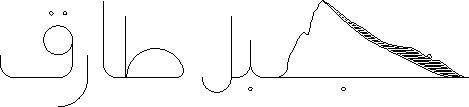
\includegraphics[width=\textwidth]{gibraltar.pdf}
    \captionsetup{labelformat=empty}
    \caption[Idéotexte de \autonym{Gibraltar} (\textarabic{جبل طارق})]{}
    \index{Urbanité}
  \end{figure}


  L’expérience humaine que constituerait ce projet s’en retrouverait enrichie de la réticence qu’ont d’ordinaire les gens à se faire photographier par un inconnu autant que de la gageure qu’il y’aurait à relever ce défit en négociant au travers du double vitrail qui les sépare du photographe.
  Du fait de l’aspect hirsute que me conférait alors ma barbe noire quelques trois mois après que j’eu cassé ma tondeuse, je me dis qu’il faudrait préparer des écriteaux à l’avance.

  L’un dirait par exemple :

  \begin{quotation}
    M’autoriserez-vous, je vous prie à vous photographier ?
  \end{quotation}

  Nous pourrions même ajouter afin de mettre en confiance compte à nos intentions :
  \begin{quotation}
    Je suis artiste et fais une série de portraits dans le train.
  \end{quotation}

  À ce point, la malice me suggéra même d’anticiper d’éventuels refus en prévoyant un second écriteau qui rassurerait de la façon suivante :

  \begin{quotation}
    Ce n’est pas grave vous êtes gentil quand même \fallback{😺}
  \end{quotation}

  Et probablement qu’attendris ou pris de repentir, les quelques récalcitrants se raviseront. Avec un peu de chance le feront-ils avant que nos trains ne repartent dans des sens différents.
\end{prose}

\section*{Rabat}
\markboth{}{Rabat}
\addcontentsline{toc}{section}{Rabat}

\poemtitle{Sur les étoiles}\index{Astronomie}\index{Epique@Épique}\index{Astronomie!Etoiles@Étoiles}
\setIndexNameEntry[Sur les etoiles]{Sur les étoiles}
%\setIndexNameEntry[]{}
\begin{verse}\sizain
  \rhyme[ere]{ère}%
  \rhyme{oir}%
  \rhyme{eur}%
  \rhyme{oile}%
  \rhyme{voi}%
  \rhyme{teur}%
  \rhyme{lite}%
  \rhyme{osse}%
  \rhyme{heur}%
  Dans ma nuit solitaire\index{Nuit}\index{Insomnie},\\ \metric{6}
  Ton visage stellaire\\ \metric{6}
  Transperce le long soir\\ \metric{6}
  Et m’apporte un espoir.\\ \metric{6}
  Car sous quelques lueurs\\ \metric{6}
  Tu raviras ma peur.  % 6

  Circulant sur l’étoile,\\ \metric{6}
  Un éclair se dévoile\\ \metric{6}
  Et éclaire ma voie\\ \metric{6}
  Celle où j’entends ta voix.\\ \metric{6}
  Qui m’attire comme un vecteur.\\ \metric{8}
  Car tu es mon navigateur.  % 7

  D’entre les satellites,\\ \metric{6}
  S’est érigée l’élite\\ \metric{6}
  Qui s’engage précoce\\ \metric{6}
  Dans le fond du cosmos.\\ \metric{6}
  Ne nous entrave aucun heurt\\ \metric{7}
  Et nous y allons sur l’heure.  % 7
\end{verse}

\poemtitle{L’armée de cils}\index{Epique@Épique}
\setIndexNameEntry[armée de cils]{L’armée de cils}
%\setIndexNameEntry[]{}
\begin{verse}\quatrain
  \rhyme[e]{é}%
  \rhyme[epic]{épic}%
  Fallait-il que ses cils soient une armée\index{Femmes}\\ \metric{10}
  Dont les phalangistes\index{Guerre} lèvent les pics\\ \metric{10}
  Aux pointes si acérées qu’en une volée\index{Archerie}\\ \metric{12}
  Se fait craindre un regard de profondeur épique\index{Femmes!Yeux}.\\ \metric{12}
\end{verse}

\begin{figure}[h]
  \centering
  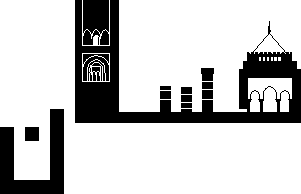
\includegraphics{hassan-monochrome.pdf}
  \captionsetup{labelformat=empty}
  \caption[Idéotexte de la tour \autonym{Ĥassān} (\textarabic{حسان})]{}
  \index{Architecture}
\end{figure}

\begin{prose}
  J’écrivis les lignes qui suivent alors que j’étais attablé à un établissement de l’avenue Patrice Lumumba, en plein milieu d’une harassante journée de travail, tandis que le soleil caressait de quelques rayons dont la rigueur pouvait s’épargner pour peu que l’on s’en convainquit.
L’une de ces étranges journées où l’ensoleillement se trouve dans un équilibre précaire qui daigne accorder aux hommes, à condition d’application mentale, le choix entre les douceurs d’une chaleur avenante et les morsures scélérates d’un brulant incendie.

  Je me souviens que ce jour là, comme à mon habitude, je me mis à la table proche du palmier d’où de temps à autre tombaient quelques noies dont le bruit de la chute faisait un agréable tapotement. Je noyais alors ma fatigue dans un café noir qu’accompagnait un onctueux paris-brest (la chose a son importance). Mais, trêve de \xenism{story-telling} qui tourne à l’exhibition d’une \xenism{instagrameuse} pré-pubère \incise{quoiqu’il me faut vous expliquer impatients lecteurs ces conditions}. Toujours est-il que je laissais couler les précieuses gorgées du seul et véritable or noir lorsqu’arriva splendide une jeune femme dans sa démarche majestueuse qui, en osmose avec les tons beige, ambré et alezan de la décoration du lieu, par une soudaine synesthésie risqua de me la faire confondre avec ma boisson. Que je manquai d’avaler de travers, d’ailleurs.

  En un laps mon esprit vacilla et ne pu honnêtement plus distinguer ces deux entités, tant il y avait là identité. Et les rayons ardent de l’archer héliaque haut juché qui jusqu’à lors trébuchaient sur ma cuirasse dermique parvinrent, à la faveur de la faiblesse naissante, à me transpercer la peau. M’épongeant le front, il me fallut par de laborieux efforts me ressaisir mais ce fût alors au prix d’une contrepartie des plus voluptueuses. Que tous les incidents, différents, discordes, et difficultés puissent se résoudre de la sorte\,!

  Car raisonna en mon esprit une entrainante musique\index{Musique} qui voulut clamer, par les joyeuses percutions d’une fanfare, la gloire de l’arrivée de cette belle, et dont les paroles me vinrent naturellement, comme dictées par la nécessité de célébrer une suavité fière qui ne pouvait souffrir aucune patience. Plût au Ciel que mon lettrisme eusse pu suffire à transcrire le solfège afin de vous apporter l’air que j’entendis. Mais si je ne peux vous rapporter le son alors au moins ne vous laisserais-je ni aveugle, ni anesthésique, ni même agueusique  de la peau de cette élégante quoique portant un voile faisant des pétales de caféiers autour de son pistil de visage (je sais le lieu commun éculé depuis Gérard \textsc{de Nerval}\index{Fleur!Cliché de \textsc{De Nerval}} mais il est ici irrésistible), qui me sembla aussi onctueuse que la mousseline de mon paris-brest tandis que la fierté que l’on lisait dans ses yeux rivalisait d’âcreté avec le café.

  Il y avait grande adresse dans la lenteur pourtant célère de ses mouvements souples qui nous confinent à l’oxymore. Jambe après jambe, elle faisait accorder sa taille élancée au balancement de  ses épaules dans un rythme si parfait que j’en fus bouleversé. Un évènement eut lieu ce jour là. Je pourrais encore poursuivre sur la description du ravissement qui fût mien et vous dire que, dès que je fini le travail, en fait de mon entrainement quotidien aux armes, ce fût un qalām\index{Ecriture@Écriture!Qalām} dont l’encre, tel que le rapporte le ĥadith\index{Islam}, est plus sacrée que le sang\index{Guerre!Sang} du martyr, que je dus encocher à mon arc\index{Archerie} lorsque je  me précipitais le soir même pour peaufiner et ciseler encore ce poème qui me teint éveillé jusque tard dans la nuit. C’est que cette dame se confondit avec la boisson qui excite jusque dans ses effets métaboliques.
\end{prose}



\poemtitle{La ravissante boisson}
\setIndexNameEntry[ravissante boisson]{La ravissante boisson}
%\setIndexNameEntry[]{}
\setIndexNameEntry[ravissante boisson]{La ravissante boisson}
\begin{verse}\quatrain
  \rhyme{tile}%
  \rhyme{ense}%
  \rhyme[oizie]{o[i\textpipe{}u]zie}%
  \rhyme[e]{é}%
  \rhyme{orge}%
  \rhyme{ombre}%
  \rhyme[ere]{ère}%
  \rhyme[ame]{a[r]me}%
  \rhyme{oir}%
  \rhyme{ure}%
  \rhyme[ere]{ère}%
  \rhyme[ante]{[a\textpipe{}e]nte}%
  \rhyme{reine}%
  \rhyme[e]{é}%
  \rhyme{our}%
  \rhyme[eo]{éo}%
  \rhyme{ante}%
  \rhyme[e]{é}%
  \rhyme[esse]{èsse}%
  \rhyme[eme]{ème}%
  \rhyme{anse}%
  \rhyme[e]{é}%
  \rhyme{i}%
  \rhyme[este]{èste}%
  \rhyme{iaire}%
  Ô puissant arôme subtile,\\ \metric{8}
  Sans lequel tout est futile,\\ \metric{7}
  Toi qui enchantes mes sens\\ \metric{7}
  Pareil à celle qui s’avance,\index{Café!Café personnifié en femme}  % 8

  Toi qui fais jalouser l’ambroisie,\\ \metric{9}
  Que le bachique\index{Café!Rivalité Café-Alcool}\endnotemark[\getrefnumber{foot.xayam}] ne saurait suspecter,\\ \metric{11}
  Exhale les doux parfums d’Andalousie\index{Al\,Andalous}\\ \metric{11}
  Qui nous font hisser nos gobelets,  % 9

  \BrText{%
    Et coule, coule le long de ma gorge.\\ \metric{10}
    Abreuve-moi de tes exquises ombres\\ \metric{10}
    Qui ruissellent le long de ton corps sombre,\\ \metric{10}
    Tel le fer en fusion dans la forge.  % 10

    Ondoie, flamme\index{Feu} singulière,\\ \metric{7}
    Lorsque le vent frais te flaire,\\ \metric{7}
    De tes torrents de charme\\ \metric{6}
    Qui torréfient mon âme  % 6
  }

  En place du véritable or noir,\\ \metric{9}
  L’huile de pierre\endnote{L’\autonym{huile de pierre}, décrite au vers précédent comme \autonym{or noir}, désigne la \xenism{petra oleum} ou pétrole.}\label{foot.huiledepierre}, en imposture,\\ \metric{8}
  Se dressa pour se faire voir,\\ \metric{8}
  Mais ne peut en emprunter l’allure.  % 9

  Car si du nectar du désert\endnotemark[\getrefnumber{foot.huiledepierre}]\\ \metric{8}
  La vile engeance prolifère,\endnote{Allusion à l’aphorisme selon lequel \enquote{les conflits prolifèrent dans les zones pétrolifères}.}\\ \metric{8}
  De tes effluves apaisantes\\ \metric{8}
  Nous ne goûtâmes que l’entente.  % 8
\AddToShipoutPictureFG*{%
  \begin{textblock*}{3cm}(12.5cm,16.5cm) 
    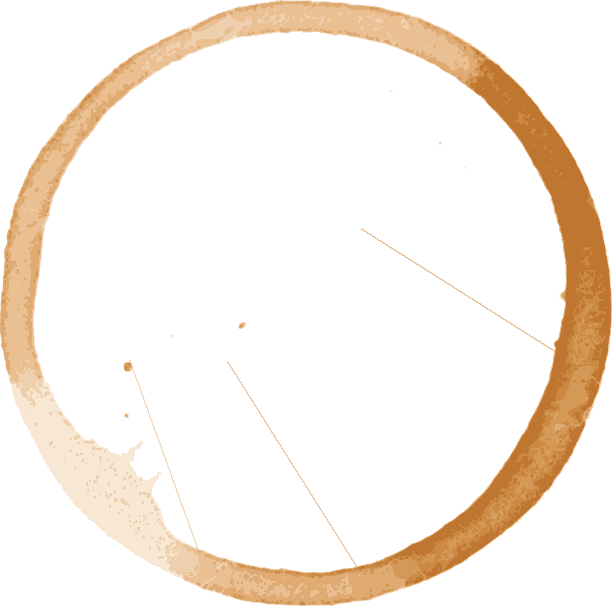
\includegraphics[height=3cm]{culacino.pdf}
  \end{textblock*}
  }

  \emph{Refrain}  % 

  Et suis, café, de tes odeurs enivrantes\\ \metric{11}
  La noble procession de la reine\\ \metric{10}
  À la couronne sertie de tes graines\\ \metric{10}
  Qui a ravi au caroubier\endnote{Les graines de caroubier, du fait de leur masse extrêmement régulière de 22\,g, servirent d’étalon dans la joaillerie et sont à l’origine de l’unité de mesure dite \emph{carat}.} la patente.  % 11

  Que le barista manie son levier\\ \metric{10}
  Et le serveur diffuse ton encens.\\ \metric{10} % TODO problème de rime
  La voici, au chemisier couleur lait,\\ \metric{10}
  Dans sa démarche quintessenciée.  \metric{10} 

  \emph{Refrain}  % 

  Traversant les rangés de table sur la cours,\\ \metric{12}
  Sur mes lèvres, coule ta robe de velours.\\ \metric{12}
  Qui projette sur le verre une vidéo\index{Photographie}\\ \metric{12}
  Tandis que tes flots s’oient en dolby stéréo.\index{Technique}\index{Cinéma}  \metric{12}

  Amante, tu es la sultane vivante\\ \metric{11}
  Qui domine cette maison de café\index{Café!Etablissement cafe@Établissement café}\\ \metric{11}
  Des quelques sveltes volutes odorantes\\ \metric{11}
  Qu’y imprime ta démarche raffinée. \metric{11}

  \emph{Refrain}  % 

  Bel orbe, à toi la grâce et à moi l’ivresse.\\ \metric{11}
  Latte macchiato au chemisier blême,\\ \metric{11}
  Tes mouvements emplis de tant de promesses\\ \metric{11}
  Incitent nonchalamment ma lente plume à déborder du poème. \index{Propos réflexif}\metric{18}

  Adam et Ève\index{Bible} qui causèrent notre errance\\ \metric{12}
  Jusqu’à sacrifier l’Éden au seul pommier,\\ \metric{12}
  Auraient dû prendre le fruit du Rubiacé\endnote{En l’occurrence le caféier qui est de la famille des Rubiacés.}\\ \metric{12}
  Car tel est le seul arbre de la connaissance. \metric{12}

  \emph{Refrain}  % 

  Tu m’ôtes le sommeil, m’éveilles, m’extasies,\\ \metric{12}
  Et m’attire de ton lien dans la nuit\\ \metric{11}
  Où la noirceur de l’espresso céleste\\ \metric{10}
  N’est parsemée que de sucre leste. \index{Astronomie!Etoiles@Étoiles}\metric{9}

  Lorsque de ton voile tu te délestes,\\ \metric{10}
  Je crois voir du liégeois la crinière,\\\index{Femmes!Cheveux} \metric{10}
  Napée de caramel qui en un geste\\ \metric{10}
  Trouve de ma bouche l’itinéraire. \metric{10}

  \emph{Refrain}
\end{verse}


\begin{prose}
  Je ne peux hélas rien vous cacher. Dans la \work{Cantate du café} de Sébastien \textsc{Bach}\index{Artistes!Sebastien@Sébastien \textsc{Bach}}, je suis Lieschen. Que j’aurais voulu être à la maison de café Zimmerman à Leipzig où j’arguerais d’une voix soprano combien  cette boisson est assurément l’ambroisie. Et pour paraphraser Sacha \textsc{Guitry} quoiqu’au sujet, non pas de \textsc{Mozart} mais de \textsc{Bach}, ô privilège du délice, lorsque la boisson se tarit, la vacuité était encore d’elle.
\end{prose}

\begin{figure}[h]
  \centering
  
\includegraphics[width=0.33\textwidth]{cigarette.pdf}
  \captionsetup{labelformat=empty}
  \caption[Idéotexte de la \autonym{cigarette}]{}
\end{figure}

\poemtitle{La boisson}
\setIndexNameEntry[boisson]{La boisson}
%\setIndexNameEntry[]{}
\begin{verse}\sizain
  \rhyme{ic}%
  \rhyme[coupe]{c[r]oupe}%
  \rhyme{vide}%
  Geste ô combien cinématographique\index{Cinéma}\index{Café}\\ \metric{10}  % 
  Qui du briquet n’envie pas l’esthétique.\\ \metric{10}  % 
  Saisissant la tasse à la belle croupe\index{Café!Café personnifié en femme},\\ \metric{10}  % 
  C’est aux cieux que je lève cette coupe.\\ \metric{10}  % 
  Pour l’élégance, je porte à la lèvre avide\\ \metric{12}  % 
  Mon verre de café depuis bien longtemps vide. \metric{12}
\end{verse}

\poemtitle{De l’attablée}
\setIndexNameEntry[attablée]{De l’attablée}
\begin{verse}\haiku
  \rhyme[e]{é}%
  Assise au café,\index{Café!Etablissement cafe@Établissement café}\\  % 
  C’était elle la boisson\index{Café!Café personnifié en femme}\\  % 
  Que je sirotais.
\end{verse}

\begin{prose}
Là, je fis une rencontre, assurément des plus charmantes, celle de mademoiselle F*****.
\end{prose}



\poemtitle{Bout des doigts}
%\setIndexNameEntry[]{}
\begin{verse}\tercet
  \rhyme{eur}%
  Lorsqu’à peine de ses doigts elle m’effleure.\index{Femmes}\\ \metric{11}  % 
  Ô nuit\index{Nuit}, ô yeux\index{Femmes!Yeux}, ô yeux, ô nuit\endnotemark[\getrefnumber{foot.vocaliseYeuxNuit}]\\ \metric{8}  % 
  C’est une pluie\index{Eau} qui ravit par sa fraîcheur. \metric{11}
\end{verse}

\begin{figure}[h]
\centering

\includegraphics[width=0.33\textwidth]{pluie.pdf}
\captionsetup{labelformat=empty}
\caption[Idéotexte de la \autonym{pluie}]{}
\end{figure}

\poemtitle{Clausewitz sur la redoute}\index{Guerre!Stratégie}\index{Guerre!Généraux historiques}
%\setIndexNameEntry[]{}
\begin{verse}\quatrain
  \rhyme{in}%
  \rhyme[tination]{tin[u]ation}%
  \rhyme{isse}%
  Te croyais-tu sur la redoute\index{Histoire!Modernité}\endnote{Allusion à la redoute Raïevski dans laquelle se trouvait le général \textsc{Clausewitz} d’après ses écrits lors de la bataille de la Moskova—Borodino.} si malin ?\\ \metric{12}  % 
  {Clausewitz}, je  dis à ta destination :\\ \metric{12}  % 
  \enquote{La guerre n’est que la continuation\\ \metric{12}  % 
  De l’amour par d’autres moyens.\endnote{Allusion à la maxime phare de l’analyse clausewitzienne \enquote{La guerre n’est que la continuation de la politique par d’autres moyens} dans son ouvrage \work{De la guerre}.}} \metric{8}

  Était-ce pour de la politique qu’Ulysse\index{Mythologie grecque!Troie}\\   \metric{12}% 
  Mit à profit  l’immensité de sa métis\index{Guerre!Ruse}\endnote{Qualité relative à l’intelligence sociale attribuée à Ulysse. À raprocher de la ruse.},\\   \metric{12}% 
  Et que tous les Achéens\endnote{Les Grecs, énemis des Troyens.} périrent en lice ?\\   \metric{12}% 
  Ou était-ce pour ravir Hélène à Pâris ?\index{Amour} \metric{12}
\end{verse}

\poemtitle{Du battement de lèvres}
\setIndexNameEntry[battement de lèvres]{Du battement de lèvres}
\begin{verse}\haikuIII
Zygène étend ses deux ailes\\  % 
Prête à s’envoler\\  % 
N’était qu’un sourire.
\end{verse}

\poemtitle{Fruits rouges}
%\setIndexNameEntry[]{}
\begin{verse}\quatrain
  \rhyme{on}%
  \rhyme{raize}%
  Myrtille, framboise, fruit de la passion,\\  \metric{12}% 
  Dégustons les délices de l’instant de braise.\index{Feu}\\  \metric{12}% 
  Sans le moindre égard pour tous les qu’en-dira-t-on,\\  \metric{12}% 
  Nous croquerons bien encore cerise et fraise. \metric{12}
\end{verse}

\poemtitle{Le trait}\index{Epique@Épique}
\setIndexNameEntry[trait]{Le trait}
\begin{verse}\quatrain
  \rhyme{gar}%
  \rhyme{isse}%
  \rhyme[e]{é}%
  \rhyme{endi}%
  \rhyme{i}%
  \rhyme[ere]{ère}%
  Elle se retourna dans un furtif regard\index{Femmes!Yeux}\\  \metric{12}% 
  Que vite je saisi dans l’instant subreptice\\   \metric{12}% 
  En l’assassinant d’un de mes traits qui égarent\index{Archerie}\\   \metric{12}% 
  Mais qui ricochât sur son œil plein de malices. \metric{12}

  À peine les flèches eurent-elles sifflé,\\   \metric{12}% 
  Que déjà dans le tronc d’arbre elles sont fichées.\\   \metric{12}% 
  Et tel la grise fumée  qui suit  l’incendie\index{Feu},\\   \metric{12}%  % TODO accord de tel
  L’ultime bourdonnement enfin s’entendit. \metric{12}

  Et des cercles concentriques de sa pupille\\   \metric{12}% 
  Que l’on crut cible mais qui se révèle archère,\\   \metric{12}% 
  Parti la verbération qui fendit l’air\\   \metric{12}% 
  Et c’est dans mon cœur que le bourdonnement s’ouït. \metric{12}
\end{verse}



\poemtitle{De l’heureux jardin}\index{Jardins}
\setIndexNameEntry[heureux jardin]{De l’heureux jardin}
\begin{verse}\haiku
  \rhyme{eu}%
  Au jardin heureux,\\  % 
  Par dessus le tapis  vert,\\  % 
  S’étend le ciel bleu.
\end{verse}

\poemtitle{Noces macabres d’Antigone et Hémon}\index{Mythologie grecque}\index{Amour}
%\setIndexNameEntry[]{}
\begin{verse}\quatrain
  \rhyme{aman}%
  \rhyme[ambo]{[a\textbar{}o]mbo}%
  \rhyme{fer}%
  En criant emmurée dans la grotte, l’âme en\\  \metric{12}% 
  Peine, tu attires cependant ton amant.\\  \metric{12}% 
  Et celui qui accourt vers toi tel un aimant,\\  \metric{12}% 
  Pour se joindre à ta mort, celui-là est Hémon.\metric{12}

  Le lit nuptial se sculpte dans le tombeau\\  \metric{12}% 
  Là où l’hymen ne sera jamais en lambeau,\\  \metric{12}% 
  Et ce que noue Vénus survivra aux enfers\\  \metric{12}% 
  Car Hadès, lui même, ne saurait le défaire. \metric{12}
\end{verse}

\poemtitle{Récollection}
\setIndexNameEntry[Recollection]{Récollection}
\begin{verse}\quatrain
  \rhyme{oir}%
  \rhyme[van]{v[a\textbar{}e]n}%
  Nous aimons nos morts, nous louons leur mémoire,\\  \metric{11}% 
  Et les chérissons bien plus que les vivants\\  \metric{11}% 
  Sans doute est-ce parce que bien moins souvent\\  \metric{11}% 
  Ont-ils l’occasion de nous décevoir.\metric{11}
\end{verse}

\poemtitle{Le secrêt}\index{Epique@Épique}
\setIndexNameEntry[secret]{Le secrêt}
\begin{verse}\quatrain
  \rhyme{i}%
  \rhyme[e]{é}%
  Ce qui n’a pas su être dit,\\  \metric{8}% 
  Ce qui ne le sera jamais,\\  \metric{8}% 
  C’est dans l’ombre qu’il s’y ouït\\  \metric{8}% 
  Et s’en entendent les méfaits.\metric{8}
\end{verse}

\poemtitle[ln 3, la plus belle de toutes]{\mathversion{bold}$\ln{3} $\mathversion{normal}, la plus belle de toutes}
\setIndexNameEntry[ln 3 la plus belle de toutes]{ln 3, la plus belle de toutes}
%\renewcommand\currentpoemtitle{ln 3, la plus belle de toutes}%
\index{Mythologie grecque!Troie}
\begin{verse}\quatrain
  \rhyme{a}%
  \rhyme{atre}%
  Personne ne sait ce qui se passa,\\ \metric{10} % 
  À la suite de la guerre de Troie\\  \metric{10}% 
  Mais je vais vous le dire sans  débattre\\  \metric{10}% 
  Ce qui eu lieu, c’est la guerre de Quatre.\metric{10}
\end{verse}

%\paragraph{}
\begin{prose}
Je promis à F***** de venir la voir à Eljadida dès après \fallbackserif{Ȝ}īd al\,Aḋĥā.
\end{prose}

\begin{prose}
  Mais pour l’instant, sous les murailles de la vieille ville de Salé\index{Architecture}, m’apparurent de jeunes filles qui quoiqu’emmitouflées dans des ĥaïks, n’en demeuraient pas moins coquettes avec leurs vêtements contemporains en dessous. D’improbables chaussures à talons aux couleurs vives pointaient même à l’endroit du… un clapsus faillit me faire écrire \enquote{piédestal}.
\end{prose}


\begin{figure}[h]
\centering
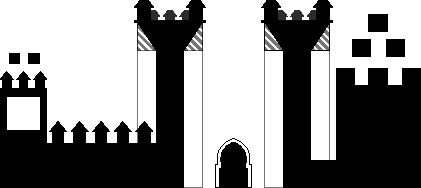
\includegraphics[width=0.30\textwidth]{chellah.pdf}
\captionsetup{labelformat=empty}
\caption[Idéotexte du \autonym{Chellah} (\textarabic{شالة})]{}
\end{figure}

\newpage{}
\begin{textblock*}{8cm}(0.5cm,3cm) 
\poemtitle{Ĥaïk}
\setIndexNameEntry[haik]{Ĥaïk}
\begin{verse}\quatrain
  \rhyme{ame}%
  \rhyme[adille]{a[d\textbar{}b]ille}%
  \rhyme[ance]{an[c\textbar{}ch]e}%
  \rhyme[ere]{ère}%
  \rhyme{deur}%
  \rhyme[te]{té}%
  \rhyme[esse]{èsse}%
  \rhyme[en]{[e\textbar{}o]n}%
  \rhyme{tus}%
  \rhyme{rine}%
  \rhyme{ssage}%
  \rhyme{ol}%
  Soutenant du dessus du blanc \xenism{litham}\endnote{Bande d’étoffe couvrant la partie basse du visage des femmes, juste en dessous des yeux.}\label{foot.litham}\\  \metric{10}% 
  Un regard\index{Femmes!Yeux} insolent de peccadille,\\  \metric{10}% 
  Mystère du tissus qui déshabille\\  \metric{10}% 
  Davantage qu’il ne vêtit les femmes.\metric{10}

  Ce triangle frontal de chaire blanche\\  \metric{10}% 
  Au haut pyramidion capillaire\\  \metric{10}% 
  Est peau de chagrin pleine de lumière\\  \metric{10}% 
  Où s’agrippent de lestes espérances.\metric{10}

  Une obscénité qui se fit pudeur\\  \metric{10}% 
  Serti le visage décolleté,\\  \metric{10}% 
  Et à l’endroit où l’on retient l’ardeur\\  \metric{10}% 
  Crée une si nouvelle nudité\metric{10}

% Là, la pupille qui pointe en téton,\\  \metric{10}% 
% S’aréole de khôl. Quand il se baisse,\\  \metric{10}% 
% Soustrait aux regards ses délicatesses,\\  \metric{10}% 
% Opposant des sourcils en un auvent.\metric{10}

  Car là, son iris qui pointe en téton, \\  \metric{10}% 
  Aréolé de khôl qu’il est, se baisse, \\  \metric{10}% 
  Soustrait aux regards ses délicatesses, \\  \metric{10}% 
  Et oppose des sourcils en auvent.  \metric{10}% 

  Et sourcils effilés jusqu’au canthus,\\  \metric{10}% 
  En un ongle lacérant ma poitrine\\  \metric{10}% 
  Qui est alors l’âtre où siège, chagrine,\\  \metric{10}% 
  La flamme aux feuilles tissées de lotus.\metric{10}

  Resplendissants et glorieux visages,\\  \metric{10}% 
  Pistils des femmes emplis de présages\\  \metric{10}% 
  Aux cheveux \index{Femmes!Cheveux}sépales qu’elles cajolent,\\  \metric{10}% 
  Se sont-ils adjoint pareilles corolles ?\metric{10}
\end{verse}
\end{textblock*}
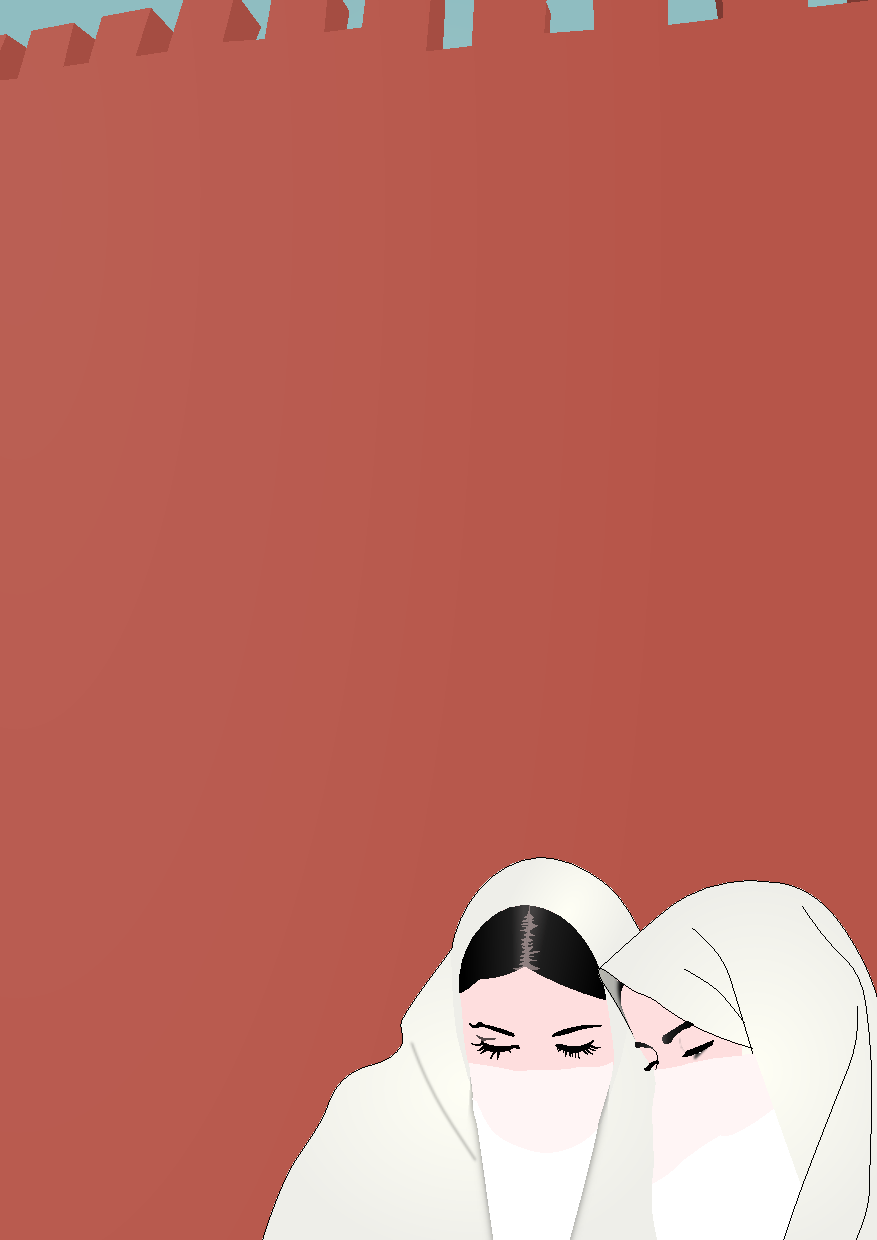
\includepdf[pages={1},addtolist={1,figure,{Mademoiselle F***** au sourcil encoché},encoche}]{haik-pleine-page.pdf}


\poemtitle{La fleur}\index{Fleur}
\setIndexNameEntry[fleur]{La fleur}
\begin{verse}\quatrain
  \rhyme{in}%
  \rhyme{emen}%
  \rhyme[e]{é}%
  \rhyme{ire}%
  M’enlisant dans le lieu commun\\\index{Propos réflexif}  \metric{8}% 
  Que tous les scribouillards crétins\\  \metric{8}% 
  Ont épuisé jusqu’à l’écœurement,\\  \metric{10}% 
  Je prétend en faire un ravissement.  \metric{10}% 

  Car la fleur que je ne peux emporter\\  \metric{10}% 
  Je l’admire  sans pouvoir la cueillir.\\  \metric{10}% 
  Et si l’étreinte,  la ferait périr\\  \metric{10}% 
  Gérard de Nerval\index{Artistes!Gérard \textsc{de Nerval}}\index{Fleur!Cliché de \textsc{De Nerval}}, saura m’excuser.  \metric{10}% 
\end{verse}


\poemtitle{Des cliquetis}
\setIndexNameEntry[cliquetis]{Des cliquetis}
\begin{verse}\haiku
  \rhyme{ic}%
  Cliquetis claudiquent\\  % 
  Sur le cadran métallique\\  % 
  Avec conséquence.
\end{verse}

\begin{prose}
  J’écrivis le poème qui suit sous l’influence de la figure de Lissān~al\,Ḋḋīne ibn~al\,Xatīb\index{Al\,Andalous!Lissān~al\,Ḋḋīn ibn~al\,Xatīb} et particulièrement de son muwacaĥ \work{Jadaka al\,ṙaytu} que je venais de découvrir à la faveur d’un enthousiasme naissant pour la faste période d’al\,Andalous et de l’intérêt impérieux que j’en nourris encore. Il me sembla que certaines associations, tournures et images qui, sans doute, n’influencèrent pas littérature française contrairement à d’autres œuvres arabes, méritaient d’être filées et ciselées encore. Je ne pus alors résister à la puissance des images qui fleurissent dans ses poèmes, à l’écoute desquels un oud\index{Musique!Oud} se met entre mes mains et me voilà assis sur le rebord d’une fenêtre de l’Alhambra\index{Al\,Andalous!Alhambra} à contempler l’immensité de la péninsule hibérique conquise aux Goths. De Tariq ibn~Ziyyād\index{Al\,Andalous!Tariq ibn~Zayad} à la Reconquista\index{Al\,Andalous!Reconquista}, mais bien au delà à travers l’influence qu’eut cette partie de Dar al\,Islam sur les troubadours, c’est toute al\,Andalous que je tiens d’un seul tenant. Et alors abu\,\fallbackserif{Ȝ}abd~Allah Mohammad {I}\ier{}\index{Personnages historiques!Abu\,\fallbackserif{Ȝ}abd~Allah Mohammad {I}\ier{}} ne croyait pas si bien dire, \xenism{Wa lā ṙāliba illā-llāh}, \enquote{Et il n’y a de vainqueur qu’Allah}.

%Quoique la chose ne fût pas au départ volontaire, mais finit par s’imposer, une métaphore filée du thème de l’astronomie traverse cet écrit.
\end{prose}

\poemtitle{L’horizon élégiaque}\index{Astronomie}\index{Epique@Épique}
\setIndexNameEntry[horizon elegiaque]{L’horizon élégiaque}
\begin{verse}\dizain\huitain\sizain\neuvain\quintil\septain\quatrain
  \rhyme[ere]{ère}
  \rhyme{or}
  \rhyme{o}
  \rhyme{euze}
  \rhyme[gere]{g[u]ère}
  Enrobé dans la noirceur ordinaire\index{Insomnie},\\ \metric{10} % 
  De mes nuits\index{Nuit} si longues et solitaires,\\  \metric{10} % 
  Je béni celui-là qui des transports\index{Amour}\\   \metric{10}% 
  N’en sait davantage que Guethenoc\index{Geste arthurienne}.\\   \metric{10}% 
  Toi, le paysan accablé d’efforts\\   \metric{10}% 
  Qu’en cette matière tu restes sot,\\   \metric{10}% 
  Que dans une ignorance bienheureuse,\\   \metric{10}% 
  Tu côtoies la stase délicieuse\\   \metric{10}% 
  Celle-là qui me sera étrangère\\   \metric{10}% 
  Comme elle le fût si souvent naguère. \metric{10}

  \rhyme{cule}
  \rhyme{o}
  \rhyme[e]{é}
  \rhyme{en}
  Car bien plus familier m’est le crépuscule\\   \metric{11}% 
  Depuis que ces attraits, de mes littoraux\index{Mer!Navigation},\\  \metric{11}% 
  Ne s’en sont approchés par un vil recul,\\  \metric{11}% 
  Sans amarre, que pour mieux s’y dérober,\\  \metric{11}% 
  Me laissant dans un abject dépouillement\\  \metric{11}% 
  De ceux qui frustrent jusqu’aux points cardinaux. \\ \metric{11}
  J’ouvrirais tous les ports à ces sentiments,\\  \metric{11}% 
  Malgré la défaveur de l’amirauté. \metric{11}

  \rhyme[e]{é}
  \rhyme[ere]{ère}
  Peu de choses je pourrais rapporter\\  \metric{10}% 
  Du ravissement où ils me laissèrent,\\  \metric{10}% 
  Sinon des bribes qui, quoiqu’oubliées\\  \metric{10}% 
  Font chanter les nations de concert,\\  \metric{10}% 
  Un évangile qui ne peut s’exposer\\  \metric{11}% 
  Ni ici sur terre ni haut dans les airs. \metric{11}

  \rhyme[ele]{èle}
  \rhyme[an]{[a\textbar{}e]n}
  \rhyme{ion}
  \rhyme[te]{té}
  Un brasier\index{Feu} rendit mon âme bien frêle.\\  \metric{10}% 
  Près de lui, le soleil\index{Astronomie!Soleil} n’est qu’étincelle\\  \metric{10}% 
  Car du voluptueux dandinement,\\  \metric{10}% 
  Paraissent de subreptices croissants\\  \metric{10}% 
  Dont la lune, de ses librations,\\  \metric{10}% 
  Ne peut que jalouser l’inflation.\\  \metric{10}% 
  Trois dimensions est une bonté\\  \metric{10}% 
  Que nous accorda la Divinité\\  \metric{10}% 
  Pour que les corps et leur rotondité\\  \metric{10}% 
  Puissent à tout loisir de se cuber. \metric{10}

  \rhyme{il}
  \rhyme{ui}
  \rhyme{teur}
  \rhyme{ctive}
  Elle qui sans pétales\index{Fleur}, dévoile un pistil,\index{Fleur!Cliché de \textsc{De Nerval}}\\  \metric{12}% 
  Dont la parjure clarté transperce la nuit,\\  \metric{12}% 
  Mais que l’on cache par des procédés habiles,\\  \metric{12}% 
  Fait danser son élégante tige qui fuit\\  \metric{12}% 
  Dans une fort captivante nyctinastie.\\  \metric{12}% 
  Sous ma vive acclamation de spectateur,\\  \metric{12}% 
  Au galant de nuit et sa fanfare olfactive,\\  \metric{12}% 
  Qui à la tombée du jour promptement s’active,\\  \metric{12}% 
  Ma sueur s’est vite mêlée à la senteur.\metric{12}

  \rhyme[e]{é}
  \rhyme[an]{[a\textbar{}e]n}
  \rhyme{ien}
  \rhyme[ere]{ère}
  La parhélie étrangère à nos contrées\\  \metric{11}% 
  Rend le vaste horizon insignifiant\\  \metric{11}% 
  Et peu me chaud d’en distinguer\\  \metric{8}% 
  Son orient, de l’occident.\\  \metric{8}% 
  Mes yeux ne se poseront plus que sur les siens\index{Femmes!Yeux},\\  \metric{12}% 
  Puissè-je me suffire d’un millénaire\\  \metric{11}% 
  Pour parcourir et le mal et le bien\\  \metric{10}% 
  De cette distance pupillaire.\endnote{%
    Aux quatre derniers vers de cette strophe qui ont une métrique dégressive en 12--11--10--9, existe une variante isométrique en alexandrin :%
    \begin{verse}%
      Mes yeux ne se poseront plus que sur les siens,\\  % 
      Puissè-je me suffire d’un seul millénaire\\%
      Pour parcourir l’étendue  du mal et du bien\\%
      Jonchant cette infinie distance pupillaire.\\%
    \end{verse}%
  }\metric{9}

  \rhyme[en]{[e\textbar{}o]n}
  \rhyme{our}
  Faut-il filer à pareille allure, ô temps ?\\  \metric{11}% 
  Veuille atténuer mon affliction\\  \metric{11}% 
  En ralentissant l’irrévocable cours,\\  \metric{11}% 
  Que je m’adonne à la contemplation,\\  \metric{11}% 
  Que j’en fixe quelques suaves contours.\metric{11}

  \rhyme{idre}
  \rhyme{u}
  \rhyme{en}
  Ô temps, toi qui n’est qu’une infâme hydre,\\  \metric{9}
  Fais du sablier une clepsydre,\\  \metric{9}
  Emplis là de tout ce  qui me plut,\\  \metric{9}
  Étanche mon inclination.\\  \metric{9}
  Car quand gronde l’incendie ardent\\  \metric{9}
  Qui brûle et puis s’accroît jusqu’aux nues,\\  \metric{9}
  Il reste grand même sous le vent, \\  \metric{9}
  Car c’est celui de l’éloignement.  \metric{9}


  \rhyme[ele]{èle}%
  \rhyme{be}%
  Maudit été, au solstice duquel\\  \metric{10}% 
  Je veux tordre l’odieux nocturlabe\index{Technique}.\\  \metric{10}% 
  Vive les longues nuits avec la belle\\  \metric{10}% 
  Où se fait leste le contour du galbe. \metric{10}

  \rhyme{nu}%
  \rhyme{rythme}%
  \rhyme{iabe}%
  \rhyme{dir}%
  Lune et soleil sous sa gorge nue,\\  \metric{9}% 
  Et dans sa pupille, en logarithme,\\  \metric{9}% 
  Se projette l’univers connu,\\  \metric{9}% 
  Dont le mouvement stellaire en rythme\\  \metric{9}% 
  Cache des galaxies au nikab.\\  \metric{9}% 
  Peu m’importe que l’on puisse médire,\\  \metric{10}% 
  Car pour la voir du zénith au nadir,\\  \metric{10}% 
  Je délaisserais bien mes astrolabes.\index{Technique}\metric{10}

  \rhyme{moin}%
  \rhyme[e]{é}%
  \rhyme{anse}%
  Que Dieu et les hommes soient témoins \\ \metric{9}
  Des larmes que j’ai souvent versées, \\  \metric{9}
  Si denses que le soir en est oint, \\  \metric{9}
  Et le ciel nocturne  constellé. \\ \index{Astronomie!Etoiles@Étoiles} \metric{9}
  Ces larmes que me fit épancher son absence \\  \metric{12}
  Débordent de la vaste tasse de café\index{Café} \\ \metric{12}
  Qui a prit les anneaux de saturne pour anse. \metric{12}
\end{verse}

\begin{figure}[h]
  \centering
  
\includegraphics[width=0.7\textwidth]{saturne.pdf}
  \captionsetup{labelformat=empty}
  \caption[Idéotexte de \autonym{Saturne}]{}
  \index{Astronomie}
\end{figure}


\poemtitle{Crépuscule écarlate}\index{Epique@Épique}
\setIndexNameEntry[Crepuscule ecarlate]{Crépuscule écarlate}
\begin{verse}\haiku
  Laps. Le samurai\index{Japon},\\  % 
  Rengainant son katana,\index{Guerre!Epee@Épée}\\  % 
  Mit les nues à sang.\index{Guerre!Sang}
\end{verse}

\poemtitle{Nohimé}\index{Guerre!Guérrières}\index{Epique@Épique}
%\setIndexNameEntry[]{}
\begin{verse}\quintil\tercet
  \rhyme[e]{é}
  \rhyme{ité}
  Nohimé,\index{Japon}\index{Guerre!Généraux historiques}\\  \metric{3}% 
  Ton nom est sur les murs gravé\index{Histoire}\index{Ecriture@Écriture},\\  % 
  Nohimé,\\  \metric{8}% 
  Ô terrible Nohimé,\\  \metric{7}% 
  Il le sera à jamais.\metric{7}

  Nohimé,\\  \metric{3}% 
  Et il l’est par le sans versé\\  \metric{8}% 
  Celui qui coagulait.\metric{7}

  Nohimé,\\  \metric{3}% 
  C’est le prix de l’éternité\\  \metric{8}% 
  Et tu t’en es acquittée.\metric{7}

  Nohimé\\  \metric{3}% 
  Ton nom est toujours évoqué.\\  \metric{8}% 
  Même loin de ta contrée,\\   \metric{7}% 
  Malgré l’ancienneté.\\  \metric{7}% 
  Nohimé. \metric{3}
\end{verse}

\poemtitle{Délire}
\setIndexNameEntry[Delire]{Délire}
\begin{verse}\haiku
  Au sommeil pesant,\index{Insomnie}\\  % 
  Nuée de corbeaux s’envole\\  % 
  N’était que mes cils.
\end{verse}

\poemtitle{Point d’insomnie}\index{Humour}\index{Propos réflexif}
%\setIndexNameEntry[]{}
\begin{verse}\quatrain
  \rhyme{li}%
  \rhyme{ol}%
  Poussé jusqu’au pied de mon lit\index{Insomnie}\\  \metric{8}% 
  Par une rêverie folle,\\   \metric{7}% 
  Je me retrouvai au sol\\  \metric{7}% 
  Comme le point tombé de l’ı. \metric{8}
\end{verse}

\poemtitle{La momie péruvienne}\index{Histoire!Préhistoire}
\setIndexNameEntry[momie peruvienne]{La momie péruvienne}
\begin{verse}\sizain\quatrain%
  \rhyme[figé]{f[l]igé}%
  \rhyme{ssaisi}%
  \rhyme{vide}%
  \rhyme{tal}%
  \rhyme{vi}%
  \rhyme{age}%
  \rhyme{mor}%
  \rhyme{able}%
  \rhyme{peur}%
  \rhyme{or}%
  Elle pétrifie autant qu’elle est figée,\index{Histoire}\\  \metric{11}% 
  Ses mains sont liées mais elle nous saisit.\\   \metric{11}% 
  D’effroi alors, car ses traits sont affligés.\\   \metric{11}% 
  Elle nous regarde nous, êtres livides,\\   \metric{11}% 
  Adressant un cris muet qui dessaisit,\\   \metric{11}% 
  Elle nous regarde de ses globes vides. \metric{11}

  Ceignant la mort en position fœtale,\\   \metric{11}% 
  Comme le nouveau-né qui vient à la vie\\   \metric{11}% 
  Elle livre par le trou occipital,\\   \metric{11}% 
  Un seul message à jamais inassouvi. \metric{11}

  Que veut-elle nous dire du fond des âges ?\\   \metric{11}% 
  Que veut-elle  de nous par delà la mort ?\\   \metric{11}% 
  Quand de ses yeux sombres et insoutenables\\ \metric{11}
  Elle nous obstrue un mystère insondable,\\ \metric{11}
  Terrifiants parce qu’emplis de remords,\\ \metric{11}
  Nous en comprenons peut-être le message. \metric{11}

  Ce qui suscite la crainte et la torpeur\\   \metric{11}% 
  Est que le repos n’est guère dans la mort.\\   \metric{11}% 
  Alors donc dis-nous tout, sans crainte ni peur.\\   \metric{11}% 
  Momie, nous écoutons ton cris insonore. \metric{11}
\end{verse}

\section*{Forêt}
\markboth{}{Forêt}
\addcontentsline{toc}{section}{Forêt}
\poemtitle{Du Gévaudan}\index{Epique@Épique}
\setIndexNameEntry[Gevaudan]{Du Gévaudan}
\begin{verse}\haiku
Des crocs scintillants\\  % 
De la Bête menaçante,\\  % 
La vallée de larmes.
\end{verse}

%\begin{prose}
%Je me rendis à la forêt de Mamora, non loin de Kénitra où je pu m’exercer à l’arc, peut avant \fallbackserif{Ȝ}īd al\,Aḋĥā.
%\end{prose}

\poemtitle{Une forêt pour mille ans}\index{Epique@Épique}
\setIndexNameEntry[foret pour mille ans]{Une forêt pour mille ans}
\begin{verse}\quatrain
  \rhyme[te]{té}%
  \rhyme{al}%
  \rhyme[antan]{[e\textbar{}a]nt[o\textbar{}a]n}%
  \rhyme[nere]{nère}%
  Le voici notre legs à la postérité\\  \metric{12}% 
  Qui verra majestueux les pouces plantés\\  \metric{12}% 
  Lorsqu’ayant atteint la hauteur impériale.\\  \metric{12}% 
  Et l’on en verra la canopée des étoiles.\index{Astronomie!Etoiles@Étoiles} \metric{12}

  Que soient  témoins les arbres qu’ici nous plantons,\\  \metric{12}% 
  Que la décennie n’en soit que le liminaire,\\  \metric{12}% 
  Que dans un siècle on dise encore \enquote{Il y a cent ans},\\  \metric{12}% 
  Que dans mille ans on commémore un millénaire.\metric{12}
\end{verse}

\poemtitle{L’archer forestier}\index{Archerie}\index{Epique@Épique}
\setIndexNameEntry[archer forestier]{L’archer forestier}
\begin{verse}\quatrain%
  \rhyme{in}%
  \rhyme{i}%
  \rhyme[e]{é}%
  \rhyme{ar}%
  \rhyme{or}%
  Ricoche brutale flèche d’airain\\  \metric{10}% 
  Sur la roche solide du sapin\\  \metric{10}% 
  Comme le boulet de l’artillerie\index{Guerre!Architecture militaire}\\  \metric{10}% 
  Qui sur la fière tour  ronde dévie.\endnote{En architecture militaire médiévale, les tours à base ronde sont connues pour être plus résistantes, notamment face au tirs d’artillerie, que les tours à base carrée.}\label{foot.tourRonde} \metric{10}

  Mais de sève de Salicacées saturée,\\  \metric{12}% 
  Enfonce-toi dans l’essence du peuplier\\  \metric{12}% 
  Qui au retour en laisse la pointe souillée\\  \metric{12}% 
  Et âcre d’une jaunâtre viscosité.\metric{12}

  Si les arbres ne peuvent nous contenter,\\  \metric{11}% 
  Tournons-nous alors et pointons le palmier\\  \metric{11}% 
  Dont le stipe amoureux accueille d’égards\\  \metric{11}% 
  Quoique, jaloux, retient fermement le dard.\metric{11}

  Reste le chêne-liège au bois que j’adore\\  \metric{11}%
  Qui, quoique par cette saison, démasclé,\\  \metric{11}%
  Est la cible dont le beau tissage accort\\  \metric{11}%
  Prend la flèche et me laisse la retirer.    \metric{11}%
\end{verse}

\poemtitle{Lendemain de bataille}\index{Epique@Épique}
%\setIndexNameEntry[]{}
\begin{verse}\quatrain
  \rhyme[an]{[a\textbar{}e]n}%
  \rhyme{ssol}%
  \rhyme{arde}%
  \rhyme[ambe]{[a\textbar{}o]mbé}%
  \rhyme{ouché}%
  \rhyme[nite]{nité}%
  \rhyme[langue]{l[a\textbar{}o]ngue}%
  \rhyme{lique}%
  \rhyme{cal}%
  \rhyme{o}%
  Faire couler tant de sang,\index{Guerre!Sang}\index{Guerre}\\  \metric{7}% 
  En fertiliser le sol,\\  \metric{7}% 
  Et s’y oindre abondamment.\\  \metric{7}% 
  Rien d’autre ne me console.\metric{7}

  Oui, le sang dont on se farde\\  \metric{7}% 
  Sur les champs où sont tombés\\  \metric{7}% 
  Les corps que j’ai enjambés\\  \metric{7}% 
  Et les charognards en harde.\metric{7}

  En compagne effarouchée,\\  \metric{7}% 
  La guerre les a couchés\\  \metric{7}% 
  Dans son lit d’éternité,\\  \metric{7}% 
  Me jetant sa vanité.\metric{7}

  L’amertume bien trop longue\\  \metric{7}% 
  Y a un goût métallique\\  \metric{7}% 
  Qui, écarlate et publique,\\  \metric{7}% 
  Pique le bout de la langue.\metric{7}

  Plus rien n’y est vertical,\\  \metric{7}% 
  Si ce n’est quelques chacals\\  \metric{7}% 
  Et l’épée\index{Guerre!Epee@Épée} dont le pommeau\\  \metric{7}% 
  Sert de perchoir au corbeau.\metric{7}
\end{verse}

\poemtitle{Du komorebi}
\setIndexNameEntry[komorebi]{Du komorebi}
\begin{verse}\haiku
  \rhyme[e]{é}%
  Branches de forêt,\index{Japon}\\  % 
  Le soleil\index{Astronomie!Soleil} sait s’y frayer\\  % 
  D’inattendus gués.\endnote{Le \xenism{komorebi} est dans la culture japonaise, le phénomène visuel par lequel les rayons du soleil se faufilent à travers les branches des arbres.}
\end{verse}

\poemtitle[Na Trioblóidi]{Na Trioblóidi\endnote{Nom en gaélique irlandais donné aux \enquote{Troubles}, c’est à dire le conflit nord-irlandais qui a ensanglanté l’Irlande des années 1960 aux années 1990.}}%
%\setIndexNameEntry[]{}
\renewcommand\currentpoemtitle{Na Trioblóidi}%
\index{Guerre}\index{Histoire!Histoire contemporaine}\index{Epique@Épique}
\begin{verse}\quatrain\sizain
  \rhyme[ele]{èle}%
  \rhyme{mi}%
  \rhyme{rone}%
  \rhyme{eur}%
  \rhyme{ira}%
  \rhyme{rira}%
  Depuis que débarqua Oliver Cromwel\index{Personnages historiques!Oliver \textsc{Cromwel}}\index{Guerre!Généraux historiques}\endnote{La domination anglaise sur l’Irlande fut rétablie à partir du débarquement d’Oliver \textsc{Cromwel} sur l’île où il instaura des lois pénales discriminatoires envers les catholiques.},\\  \metric{11}% 
  Sur ton île, avec la New Model Army\index{Guerre!Armée}\endnote{Armée de la Première révolution anglaise qui a été organisée et formée par \textsc{Cromwel} sur le modèle de ses propres troupes.}\\  \metric{11}% 
  Tu tiens toujours au nord comme à ta prunelle\endnote{Encore aujourd’hui, le nord de l’île est occupé par le Royaume-Uni.}\\  \metric{11}% 
  Quelles que soient les horreurs de l’ennemi.\metric{11}

  Avec ses bombes, et ses tanks et ses drones\endnote{%
    Allusion au refrain de \work{Zombie} des Cramberries puissamment chantée par la regrettée M\textsuperscript{me}\,Dolores \textsc{O’Riordan} au sujet du traumatisme du conflit nord-irlandais et qui dit :
    \begin{verse}
      With their tanks, and their bombs\\  % 
      And their bombs, and their guns
    \end{verse}%
  }\\  \metric{11}% 
  Il croit te tendre la main comme une sœur.\\  \metric{11}% 
  Mais c’est une infâme traîtrise du Trône\\  \metric{11}% 
  Qui tient la main droite rouge de l’Ulster\endnote{L’Ulster est une région historique de l’Irlande qui coïncide plus ou moins bien avec l’Irlande-du-Nord qui est l’entité sous domination britannique. La main droite ensanglantée en est le symbole héraldique traditionnel.}.\metric{11}

  Mais lorsqu’il s’en ira,\\  \metric{6}% 
  Nous tous l’on en rira.\\  \metric{6}% 
  Le poitín\endnote{Boisson traditionnelle irlandaise.} jaillira,\\  \metric{6}% 
  Et vainqueurs l’on boira.\\  \metric{6}% 
  Car partout l’on dira :\\  \metric{6}% 
  \enquote{Son règne périra}.\metric{6}
\end{verse}

\poemtitle{La confidente du jour}
\setIndexNameEntry[confidente du jour]{La confidente du jour}
\begin{verse}\dizain
  \rhyme[te]{té}%
  \rhyme[sance]{s[a\textbar{}e]nsse}%
  \rhyme[eye]{èye}%
  \rhyme{dé}%
  \rhyme[iye]{iyé}%
  Elle arrivait face au jour et sa clarté,\index{Astronomie!Soleil}\index{Femmes}\\  \metric{11}% 
  Emplie d’une gaieté annonçant l’été\\  \metric{11}% 
  Qui accueille le ciel et sa luminescence,\\  \metric{11}% 
  Pour se gorger de pleine réjouissance.\\  \metric{11}% 
  Les commissures de ses lèvres vermeil\\  \metric{11}% 
  Étaient bien retroussées jusqu’à ses oreilles\\  \metric{11}% 
  Comme une leste archère\index{Archerie} ayant l’arc bandé\\  \metric{11}% 
  Auquel est encoché la joie débridée.\\  \metric{11}% 
  C’était sur elle que la joie scintillait,\\  \metric{11}% 
  Mais c’était le soleil qui lui souriait.\metric{11}
\end{verse}

\poemtitle{De l’abeille}
\setIndexNameEntry[abeille]{De l’abeille}
\begin{verse}\haiku
  \rhyme{iye}%
  L’abeille grappille.\\  % 
  Posée sur la camomille\\  % 
  Est grain de beauté.
\end{verse}

\begin{figure}[h]
  \centering
  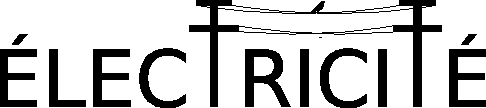
\includegraphics[width=0.6\textwidth]{electricite.pdf}
  \captionsetup{labelformat=empty}
  \caption[Idéotexte de l’\autonym{électricité}]{}
  \index{Technique}\index{Urbanité}
\end{figure}

\poemtitle{Sous les néons de la nuit}\index{Nuit}\index{Synthwave}\index{Urbanité}
%\setIndexNameEntry[]{}
\begin{verse}\quatrain
  \rhyme[ere]{ère}%
  \rhyme[iere]{ière}%
  \rhyme{rage}%
  \rhyme{i}%
  \rhyme{ui}%
  \rhyme{te}%
  \rhyme{aine}%
  Sous les néons du lampadaire,\\  \metric{8}% 
  Je suis debout et solitaire.\\  \metric{8}% 
  Et sur la flaque\index{Eau}, singulières,\\  \metric{8}% 
  S’éclaboussent tant de lumières.\metric{8}

  Là, les gouttelettes de l’éclairage\\  \metric{10}% 
  Se diffractent en nombreux clapotis \\  \metric{10}% 
  Qui dans cette rue sont l’unique bruit.\\  \metric{10}% 
  Elles ne semblent être qu’un mirage.\metric{10}

  Voile de silence que cette pluie\\  \metric{10}% 
  Abattue sur la noirceur de la nuit\\  \metric{10}% 
  Que franchi la ligne phosphorescente\\  \metric{10}% 
  De la moto que Mokoto pilote.\metric{10}

  Aussitôt suivie par de vives traînes\\  \metric{10}% 
  Que la persistance rétinienne\\  \metric{10}% 
  Conserve encore dans ma pupille.\\  \metric{9}% 
  Enfourchant sa moto, je les suis.\metric{9}
\end{verse}


\poemtitle{Fleur d’engrenage}\index{Fleur}\index{Epique@Épique}
%\setIndexNameEntry[]{}
\begin{verse}\distique
  \rhyme{age}%
  \rhyme{ol}%
  \rhyme{ile}%
  \rhyme[e]{é}%
  \rhyme{nage}%
  \rhyme[esse]{èsse}%
  \rhyme{e}%
  Tu perds tes pétales sur les chaînes d’assemblage\\  \metric{13}% 
  Où fuit ta jeunesse, toi la fleur d’engrenage.\metric{13}

  Kilomètres de câblage ont meurtri tes épaules\\  \metric{13}% 
  Qui, endolories,  sont des sépales sans corolles.\metric{13}

  Sur la liane en métal, se brise ton jeûne âge\\  \metric{13}% 
  Car pour l’industrie, tu es la fleur d’engrenage.\metric{13}

  Parce que l’on te sait belle mais fragile,\\  \metric{11}% 
  Les quolibets te trouvent cible facile. \metric{11}

  N’est-ce pas le bourdon qui prétend manager\\   \metric{12}% 
  Qui vient, tout velu, à ta tige se frotter ? \metric{12}

  Oppose à la peine et au commérages\\   \metric{10}% 
  Tes six épines de fleur d’engrenage. \metric{10}

  L’on te méprise et dédaigne, fille du câblage,\\   \metric{13}% 
  Mais au verger, tu es l’unique fleur d’engrenage. \metric{13}

  Celle que je veux arroser de richesses,\\   \metric{11}% 
  Et la seule que je comble de tendresses. \metric{11}

  Qu’à jamais se dessine la fierté\\   \metric{10}% 
  Sur les trait des visages ouvriers, \metric{10}

  De celles qui sont plus belles que les bourgeoises.\\   \metric{12}% 
  Vous qui êtes d’éclatantes fleurs d’engrenages. \metric{12}
\end{verse}

\poemtitle{Astres nourriciers}\index{Femmes}\index{Astronomie}
%\setIndexNameEntry[]{}
\begin{verse}\distique%
  \rhyme[eye]{èye}%
  Sous sa gorge qui émerveille,\\  \metric{8}% 
  Luisent la lune et le soleil.\metric{8}
\end{verse}

\poemtitle{Caresses de l’oud}\index{Musique!Oud}
%\setIndexNameEntry[]{}
\begin{verse}\quatrain
  \rhyme{oud}%
  \rhyme{ize}%
  À la première caresse de l’oud,\\  \metric{10}% 
  L’onde me fait trembler du bras au coude.\\   \metric{10}% 
  Si ma respiration s’amenuise,\\   \metric{10}% 
  Aucune autre émotion n’est permise. \metric{10}
\end{verse}

\begin{figure}[h]
  \centering
  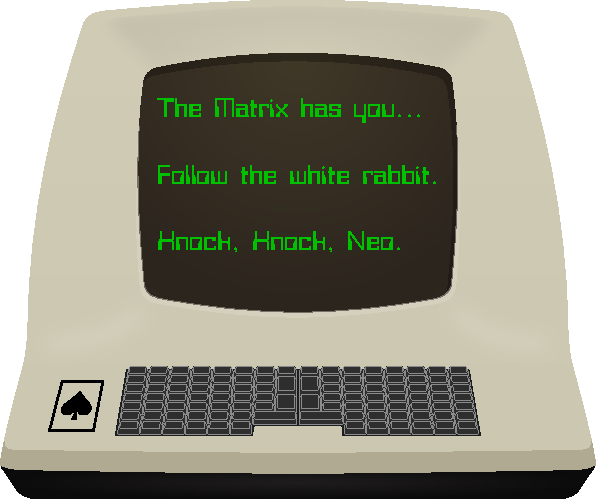
\includegraphics[width=0.30\textwidth]{adm-3a.pdf}
  \captionsetup{labelformat=empty}
  \caption[Terminal ADM-3A]{}
  \index{Technique}
\end{figure}




\poemtitle{Boucles de cheveux}\index{Femmes!Cheveux}
%\setIndexNameEntry[]{}
\begin{verse}\quatrain
  \rhyme{sage}%
  \rhyme{lon}%
  Les boucles qui encadrent son visage,\\  \metric{10}% 
  Comme autant de volutes de violon\index{Musique},\\  \metric{11}% 
  Font une si jolie chanson, en présage\\  \metric{11}% 
  De la caresse de nos doigts fêlons.\metric{10}
\end{verse}

\poemtitle{Ode du programmeur}\index{Technique}
%\setIndexNameEntry[]{}
\begin{verse}\quatrain
  \rhyme{nui}%
  \rhyme{ic}%
  \rhyme{ime}%
  \rhyme{ssoir}%
  Dans la douce noirceur de la nuit\index{Nuit},\\  \metric{9}% 
  Les gouttelettes typographiques\index{Ecriture@Écriture!Typographie}\index{Cinéma}\endnote{La \enquote{pluie de caractère} est un motif ésthétique emprunté à \work{La Matrice}.}\\  \metric{9}% 
  Ruissellent au delà de minuit\\  \metric{9}% 
  Sur mon terminal panoramique.\metric{9}

  Et les méthodes\endnote{En programmation informatique, les méthodes sont des fonctionnalités qui s’appliquent à certains objets.

  Leur enchainement dans un code informatique est semblable à celui de wagons qui s’arriment les un aux autres.
%  Une méthode pouvant elle même avoir d’autres méthodes. Dans certains langages de programmation, l’appel à une méthode sur un objet se fait en arrimant cette méthode à l’objet. Par exemple, sur l’objet \texttt{objet} s’applique la méthode \texttt{méthode} de la façon suivante : \texttt{objet.méthode}. Si une seconde méthode \texttt{méthode2} devait s’appliquer sur l’ensemble, celà prendrait la forme \texttt{objet.méthode.méthode2}.
  }
  s’enchaînent et s’arriment\\  \metric{9}% 
  Tel des wagons qui s’avancent dans le soir\\  \metric{9}% 
  Jusqu’à ce qu’une erreur ne vienne surseoir\\  \metric{9}% 
  À la course du codeur pusillanime.\metric{9}
\end{verse}

\newpage{}
\thispagestyle{empty}
\AddToShipoutPictureFG*

\section*{Intermède}
\markboth{}{Intermède}
\addcontentsline{toc}{section}{Intermède}

\poemtitle{Clapotis de l’averse}
%\setIndexNameEntry[]{}
\begin{verse}\haiku
  \rhyme{verse}%
  Avec clapotis,\index{Eau!Pluie}\\  % 
  De l’inopinée averse,\\  % 
  L’espoir se déverse.\index{Destin}
\end{verse}


\begin{prose}
  Avant \fallbackserif{Ȝ}īd al\,Aḋĥā, j’eu le plaisir de rencontrer une jeune femme que je vis d’abord, chose rare, sous son litham. Je dois admettre que ce vêtement censé repousser m’attira en réalité. Elle m’accorda même l’honneur de m’entretenir si bien que nous pûmes découvrir notre passion commune pour l’œuvre de fiction de Frank \textsc{Herbert}. Fait notable, lorsqu’elle retira son voile, je vis qu’elle avait des points de rousseur\index{Femmes!Rousseur} qui me rappelèrent le \enquote{gout de cannelle} qu’a l’épice récoltée sur Dune.
\end{prose}

\poemtitle{Litham}
%\setIndexNameEntry[]{}
\begin{verse}\quatrain
  \rhyme[ele]{èle}%
  \rhyme{ar}%
  \rhyme{coche}%
  \rhyme[an]{[a\textbar{}o]n}%
  Litham\endnotemark[\getrefnumber{foot.litham}], haute muraille\index{Guerre!Architecture militaire} aux merlons de dentelle.\\  \metric{12}% 
  D’un créneau se manifesta l’archer\index{Archerie} rebelle.\\   \metric{12}% 
  De la belle, il est l’aiguisée pupille noire\index{Femmes!Yeux}\\   \metric{12}% 
  Qui darde l’œil et est cible de mon regard. \metric{12}

  D’une fugace œillade, une seule, elle encoche\\   \metric{12}% 
  Et d’un battement de paupière elle décoche.\\   \metric{12}% 
  Toi qui de la vertu est la protection,\\   \metric{12}% 
  Tu accrois sa vulnérabilité, pourtant. \metric{12}
\end{verse}



\begin{prose}
  Et je composais alors sans doute mon première poème en arabe littéral dont je vous donnes ici la traduction qui, fatalement, sacrifie la métrique autant que les rîmes.
\end{prose}

\begin{longtable}{R{0.3\textwidth} L{0.65\textwidth}}

  \noalign{%
    \vspace{-0.5cm}\poemtitle[Dune d’Arrakis — \textarabic{كثيب أراكيس}]{\textarabic{كثيب أراكيس} — Dune d’Arrakis}%
    %\renewcommand\currentpoemtitle{Dune d’Arrakis}%
    \setIndexNameEntry[Dune dArrakis]{Dune d’Arrakis}
    \index{Dune}\index{Epique@Épique}\distique
  }

  \endfirsthead
  \vspace{0.05cm}

  \textarabic{هيبتها الأبدية}         & \vspace{0.05cm}

  Son éminence éternelle\endnote{Dans l’œuvre de fiction de Frank \textsc{Herbert}, Arrakis est une planète désertique aussi appelée par ses autochtones \autonym{Dune}.}\label{foot.DuneArrakis}\\  % 
  \textarabic{ترشدنا في الخلاء}       & Nous guide dans la vacuité\bigskip \\ 
  \textarabic{و عمرها لا يحصا}        & Elle est sans âge\\  % 
  \textarabic{لما تملأنا بالهناء.}    & Lorsqu’elle nous emplit de joie.\bigskip \\ 
  \textarabic{لكل من رأى الرمل الدائم،}  & À quiconque aura vu les sables perpétuels,\\  % 
  \textarabic{هيا مقام الصحراء.}         & Elle est l’espar du désert.\bigskip \\ 
  \textarabic{من تحت الهلالين،}      & D’en dessous des deux lunes\endnote{Autour de la planète Arrakis orbitent deux satellites naturels.},\\  % 
  \textarabic{منحنياتها تطربنا.}    & Ses courbes nous ravissent.\bigskip \\ 
  \textarabic{يا روعة الكثبان،}    & Ô magnificence des dunes,\\  % 
  \textarabic{بسموّك أملينا،}       & Empli-nous de ton excellence,\bigskip \\ 
  \textarabic{أمنحنا التسامي،}      & Dote-nous de sublimation,\\  % 
  \textarabic{بالمجد شسب عطشنا.}    & Étanche notre soif de gloire.\bigskip \\ 
  \textarabic{و الدنيا أعلنت}        & Et l’univers a déclaré\\  % 
  \textarabic{﴿من زارها زارني﴾.}     & \enquote{Qui l’aura visité m’a visité}\endnote{La planète Dune est un lieu de pèlerinage.}.\bigskip \\ 
  \textarabic{بفضل متعتك،}           & De la jouissance que tu inspires,\\  % 
  \textarabic{أزرقت أعيني.}          & Mes yeux bleuirent\endnote{L’atmosphère de Dune est saturée d’une substance appelée épice qui a de nombreux effets métaboliques sur le corps humain dont celui de rendre les yeux bleus ce que l’on nome le regard de l’\autonym{ibad}.}\label{foot.regardibad}.\bigskip \\ 
    \textarabic{في خطوط المستقبل،}   & Dans les lignes de l’avenir\index{Destin},\\  % 
  \textarabic{رأيت باطمئنان}         & J’ai vu avec quiétude\bigskip \\ 
  \textarabic{كل العقود الخبيتة}     & Que tous les nexus néfastes\\  % 
  \textarabic{نفيت في مهب الرياح.}   & Furent emportés par les vents.\bigskip \\ 
  \textarabic{في مجاري الزمان،}      & Dans les couloirs du temps,\\  % 
  \textarabic{تقدمنا و تراجعنا}     & Nous avançâmes et reculâmes\bigskip \\ 
  \textarabic{حتى فتح الممر.}        & Jusqu’à ce que se soit ouvert le passage.\\  % 
  \textarabic{ركضنا مبتهجين.}        & Nous avons galopé euphoriques.\bigskip \\ 
  \textarabic{تقيضنا نحوا الهدى،}    & Tu nous guides vers le sentier,\\  % 
  \textarabic{الهدى الذهبية.}        & Le sentier pavé d’or.\\  % 
\end{longtable}

\poemtitle{Pommettes}
%\setIndexNameEntry[]{}
\begin{verse}\quatrain
  \rhyme{oi}%
  \rhyme[e]{é}%
  Pommettes qui font rayonner la joie,\index{Femmes}\\  \metric{10}% 
  De pulpe de pêche elles sont gorgées.\\  \metric{10}% 
  Les rayons d’or s’y sont éclaboussés\\  \metric{10}% 
  Et la rosée en fait encore foi.\metric{10}
\end{verse}


\poemtitle{Le voile et le suaire}
\setIndexNameEntry[voile et le suaire]{Le voile et le suaire}
\begin{verse}\quatrain
  \rhyme[en]{[e\textbar{}o]n}%
  \rhyme[ere]{ère}%
  Maudit soit celui qui avec quelques haillons\\  \metric{12}% 
  Voudrait dérober cette œuvre à nos sentiments.\\  \metric{12}% 
  Elle ne sera ôtée de notre visière\\  \metric{12}% 
  Que lorsqu’enfin enveloppée dans le suaire.\\  \metric{12}% 
\end{verse}


\poemtitle{Andalousie, toujours}\index{Al\,Andalous}
%\setIndexNameEntry[]{}
\begin{verse}\sizain
  \rhyme{por}%
  \rhyme{ne}%
  \rhyme[ere]{ère}%
  Dans les nuits\index{Nuit} dont la noirceur drapait nos transports\\  \metric{12}% 
  Nous humions les effluves du jasmin nocturne\\  \metric{12}% 
  Tandis que les étoiles\index{Astronomie!Etoiles@Étoiles} emplissaient nos verres,\\  \metric{12}% 
  Celles que le soleil\index{Astronomie!Soleil} du matin évapore\\  \metric{12}% 
  Et avec elles, ce qui fit notre fortune\\  \metric{12}% 
  Avant que ne nous ait séparé le désert.\metric{12}
\end{verse}


\poemtitle{Pyrogenesis}\index{Guerre}\index{Epique@Épique}
%\setIndexNameEntry[]{}
\begin{verse}\quatrain
  \rhyme{uré}%
  \rhyme{arme}%
  %
  \rhyme{resse}%
  \rhyme[andre]{[a\textbar{}é]ndre}%
  %
  \rhyme{men}%
  \rhyme[ouce]{ou[r]ce}%
  %
  \rhyme[ante]{[a\textbar{}e]nté}%
  \rhyme{lence}%
  %
  \rhyme[atre]{atre}%
  \rhyme{aine}%
  %
  \rhyme{tin}%
  \rhyme{i}%
  %
  \rhyme[re]{ré}%
  \rhyme{age}%
  Comme un vieux destrier qui s’en va pâturer,\\  \metric{12}
  Et qui clôt les yeux dont s’épanchent quelques larmes,\\  \metric{12}
  Débarquent de sous mes paupières armurées\\  \metric{12}
  Les nefs\index{Guerre!Guerre navale}, les engins de siège\index{Guerre!Poliorcétique}, et le peuple en arme\index{Guerre!Armée}.  \metric{12}

  Eux qui sortent des casernes et forteresses\\  \metric{12}
  Fourmillent sur le territoire pour s’étendre,\index{Guerre!Invasion}\\  \metric{12}
  Sacrifiant à la guerre et à son ivresse\\  \metric{12}
  Le sang\index{Guerre!Sang} de chaque ennemi qu’ils s’en vont répandre.  \metric{12}

  Ils encerclent à mes ordres les bâtiments\\  \metric{12}
  Prennent les édifices, pillent les ressources ;\\  \metric{12}
  Nourriture, bois, pierre, métal et eau douce,\\  \metric{12}
  Sous les râles des humains et des bêlements.  \metric{12}

  Ces images qui persistent à me hanter\index{Guerre!Traumatisme}\\  \metric{12}
  À chaque  fois que me saisit une somnolence,\\  \metric{12}
  Avec les tambours de guerre au timbre argenté\index{Guerre!Bellisonus}\\  \metric{12}
  Sentent l’odeur de la mort et sa pestilence.  \metric{12}

  Car si je séduisis la belle Cléopâtre\index{Egypte@Égypte!Cléopâtre},\\  \metric{12}
  Et réduisis en cendre sur le Nil\index{Egypte@Égypte!Nil} albâtre\\  \metric{12}
  Les trirèmes britons des légions romaines\index{Histoire!Rome antique}\\  \metric{12}
  Qui tinrent garnison sur les plateaux et plaines,  \metric{12}

  Sur l’isthme de Corinthe je les contins,\\  \metric{12}
  Eux les Gaulois qui arrivent du lointain.\\  \metric{12}
  Tandis que les commerçants d’Anatolie\\  \metric{12}
  Apportaient poterie et dinanderie.  \metric{12}

  Exploitant les mines de fer et  les forêts,\\  \metric{11}
  J’ai épuisé les ressources et les denrées\\  \metric{11}
  Et c’est ainsi que j’atteignis le troisième âge\\  \metric{11}
  Dont les merveilles érigées font témoignage.\index{Architecture}  \metric{1"}

  Dans la savane, en Asie, ou sur les Cyclades\\  \metric{12}
  Devant les pylônes ou au pied des montagnes,\\  \metric{12}
  Je commande au peuple qui toujours m’accompagne\\  \metric{12}
  Femmes, paysans, fantassins par myriades.  \metric{12}

  Je fis cela et plus encore, vous dis-je.\\  \metric{12}
  Je fis tout cela, et je battis  des records\\  \metric{12}
  En témoignera même le tableau  des scores\\  \metric{12}
  Car mes hauts faits n’auront jamais été qu’un jeu.  \metric{12}
  \rhyme{ade}%
  \rhyme{agne}%
  %
  \rhyme{je}%
  \rhyme{cor}%
\end{verse}

\poemtitle{Arôme acre}
\setIndexNameEntry[Arome acre]{Arôme acre}
\begin{verse}\quatrain
  \rhyme{gorge}%
  \rhyme[ene]{ène}%
  Quand le café coule dans ma gorge,\index{Café}\\  \metric{9}% 
  Je le sens ruisseler sur la tienne,\\  \metric{9}  % 
  En épouser les formes troyennes\index{Mythologie grecque!Troie}\\  \metric{9}  % 
  Et les beautés dont elles regorgent.  \metric{9}
\end{verse}

\poemtitle{La surfeuse}\index{Mer}
\setIndexNameEntry[surfeuse]{La surfeuse}
\begin{verse}\quatrain
  \rhyme[el]{e[i]l}%
  \rhyme{eu}%
  M’avisant, adossée au ciel,\\  \metric{8}% 
  Sont-ce les boucles du soleil\index{Astronomie!Soleil}\\   \metric{8}% 
  Ou les rayons de ses cheveux\index{Femmes!Cheveux}\\   \metric{8}% 
  Qui volent en mèches de feu\index{Feu} ? \metric{8}
\end{verse}

\poemtitle{Pattes de velours}
%\setIndexNameEntry[]{}
\begin{verse}\quatrain
  \rhyme{tour}%
  \rhyme{our}%
  De son cou et de son pourtour,\index{Femmes}\\  \metric{8}% 
  Mes doigts  qui en tracent le contour\\  \metric{9}% 
  Sont des caresses d’araignée\\  \metric{8}% 
  Qui pose ses pattes de velours.\metric{9}
\end{verse}

\poemtitle{Les flots de la danseuse}\index{Femmes}
\setIndexNameEntry[flots de la danseuse]{Les flots de la danseuse}
\begin{verse}\quatrain
  \rhyme[oune]{ou[r]ne}%
  \rhyme[ere]{ère}%
  \rhyme{anse}%
  \rhyme[ebre]{èbre}%
  \rhyme{ien}%
  \rhyme[oma]{o[n\textbar{}m]a}%
  \rhyme{ote}%
  \rhyme[eye]{èye}%
  \rhyme{ire}%
  \rhyme[ele]{èle}%
  Dès le premier pincement du kanoun\index{Musique!Kanoun}\endnotemark[\getrefnumber{foot.kanoun}],\\  \metric{10}
  De la corde part l’onde singulière\\  \metric{10}
  Jusqu’à mouvoir le corps de la corsaire\index{Mer!Navigation}\\  \metric{10}
  Qui aborde mon âme et la détourne.  \metric{10}

  Accompagnant sa lascive danse,\\  \metric{9}
  Elle chante l’oraison funèbre\\  \metric{9}
  Qui scelle le trépas de mon innocence,\\  \metric{11}
  Et une passion secrète célèbre.  \metric{11}

  Et contrairement à l’Ithaquien\index{Mythologie grecque!Odyssée}\endnotemark[\getrefnumber{foot.ithaquien}],\\  \metric{10}
  Nul besoin de m’attacher au mat\\  \metric{9}
  Tant les charmes me nouent des liens\\  \metric{9}
  Et que toute raison m’abandonna.  \metric{10}

  Navigant sur les courbes, ma flotte\\  \metric{9}
  À chaque port ravit les merveilles\\  \metric{9}
  Car ici je suis l’oramanaute\endnote{Hapax. Du grec ὅραμα, \enquote{spéctacle} et du latin \xenism{nauta} \enquote{navigateur}. Pouvant être compris dans le sens d’\enquote{explorateur des beautés}.}\\  \metric{9}
  Qui vogue sur l’océan vermeille.  \metric{9}

  Mais d’une carte mouvante il faut me munir\\  \metric{12}
  Car la tectonique des côtes charnelles\\  \metric{11}
  Est d’une inconstance qui sait ébaudir\\  \metric{11}
  Par la souplesse que seule connait la belle.  \metric{12}
\end{verse}

\poemtitle{Grains de beauté}\index{Femmes!Rousseur}
%\setIndexNameEntry[]{}
\begin{verse}
  \rhyme[ete]{ète}%
  \rhyme{iole}%
  L’infini et l’infime se reflètent,\metric{10}\\  % 
  Dans cette poudre qui s’étiole.\\  \metric{9}% 
  Mais sont-ce étoiles\index{Astronomie!Etoiles@Étoiles} ou lucioles\\  \metric{9}% 
  Que les grains de beauté sur ses pommettes ?\metric{10}
\end{verse}

\poemtitle{Du regard}
\setIndexNameEntry[regard]{Du regard}
\begin{verse}\haiku
  \rhyme[ere]{ère}%
  \rhyme[pere]{père}%
  Ton regard sévère,\index{Femmes!Yeux}\\  % 
  Je crains autant que j’espère\\  % 
  Qu’il ne me repère.
\end{verse}


\poemtitle{Ombres des drones}
%\setIndexNameEntry[]{}
\begin{verse}\haiku
  \rhyme{oi}%
  Ses mortels convois\\
  Volent au dessus des lois.\\
  Mort et désarroi.
\end{verse}

\begin{figure}[h]
  \centering
  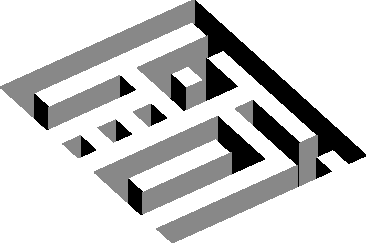
\includegraphics[width=0.3\textwidth]{hofra.pdf}
  \captionsetup{labelformat=empty}
  \caption[Idéotexte du \autonym{trou} (\textarabic{حفره})]{}
\end{figure}

\poemtitle{Exhortation au partage selon les deux espèces}
%\setIndexNameEntry[exhortation au partage selon les deux espèces]{Éxhortation au partage selon les deux espèces}
\lettrine[lines=3,slope=-.7em]{V}{ous romprez votre pain} avec plus pauvre que vous et verserez de votre outre dans la sienne afin que vous mangiez du même pain et buviez de la même eau que lui.

Et, lorsque vous vous en irez par le chemin avec la baguette de pain rompue à son extrémité, et l’outre à moitié remplie, que l’on vous demandera pourquoi il manque à la baguette une extrémité et que l’eau de l’outre ne parvient pas au buvant ; vous répondrez que l’extrémité de la baguette de pain est la garde de l’épée que vous saisîtes pour repousser le territoire du malin, et que chaque goutte d’eau dont vous aurez fait boire plus pauvre que vous est une larme arrachée au malin.
Car le sentier d’or est pavé des miettes du pain qu’on rompu les justes.

\newpage

\thispagestyle{empty}

% C’est une magnifique fleur de lotus
% Qui traverse l’Afrique en un sillage vert
% Dont la tige serpente le long du désert
% Ainsi que l’encre coule sur le papyrus.
%
% Le Fayoum qui en est la feuille bourgeonnante
% Annonce le delta dont les eaux ondoyantes
% Forment la corolle, sans plus aucun laïus.
% Ou est-ce là un pétulant mont de Vénus ?
%
% Draine le limon,
% Ô fleur rebelle
% Là où nous buvons
% Tes eaux éternelles.
%
% J’ai vu dans le flot de tes eaux
% Le reflet du vol du faucon
% Emportant et le renouveau
% Et la chute des nations.

\AddToShipoutPictureBG*{%
  \AtPageLowerLeft{%
    \begin{tikzpicture}[remember picture]
      \node (nile)  at (current page.south west)
        {\hspace{3.2cm} 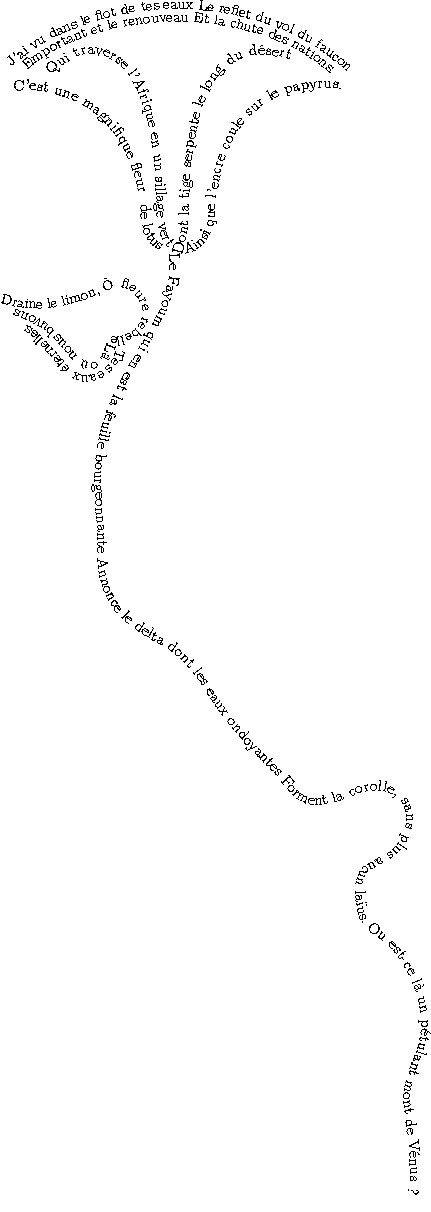
\includegraphics{nil-ajuste.pdf} };
      \node (B) at ([shift={(110:7)}]nile) {{\large\textbf{Fleur d’Afrique}%
      \renewcommand\currentpoemtitle{Fleur d’Afrique}%
      \setIndexNameEntry{Fleur d’Afrique}%
      \calligramme\quatrain%
      \rhyme{usse}%
      \rhyme[ere]{ère}%
      \rhyme{ante}%
      \rhyme{usse}%
      \rhyme{on}%
      \rhyme[ele]{èle}%
      \rhyme{o}%
      \rhyme{on}%
      \metric{12}\metric{8}\metric{5}%
        \addcontentsline{toc}{subsection}{Fleur d’Afrique}%
      }};

      \node  at (current bounding box.south west) [anchor=south west]
        {
          \hspace{0.5cm}\begin{minipage}[t][14cm][t]{8.7cm}
           \shapepar{ 
             {5}
             {0}     b{0}\\  % 
             %
             {0}     t{-1.0}{4.3}\\  % 
             {0.5}   t{-1.0}{5}\\  % 
             {1}     t{-1.0}{5}\\  % 
             {1.5}   t{-1.0}{4.7}\\  % 
             {6}     t{-1.0}{4.7}\\ % premier coude
             {7}     t{-1.0}{6.4}\\ % premier coude
             {8}     t{-1.0}{7.5}\\  % 
             %{10}    t{-1.0}{8}\\   % boucle
             {10.7}    t{-1.0}{9.9}\\ % 
             {11}    t{-1.0}{12.2}\\ % 
             {11.5}  t{-1.0}{11.2}\\  % 
             {11.6}  t{-1.0}{11.2}\\  % 
             {12}    t{-1.0}{11.0}\\  % 
             {13}    t{-1.0}{11}\\  % 
             {14}    t{-1.0}{11.7}\\  % 
             {16}    t{-1.0}{12.4}\\ % centre de l’arc
             {17}    t{-1.0}{12.0}\\  % 
             {18.5}  t{-1.0}{12.2}\\  % 
             {19}    t{-1.0}{12.3}\\  % 
             {19}    e{11}
          }%
          {\index{Egypte@Égypte!Nil}\index{Eau}\index{Fleur}\em Cette lassive \emph{fleur d’Afrique} décrit par sa tige le cours du Nil d’un point de vue zénithal tandis que le delta est figuré à la façon d’une corole de fleur de lotus selon sa représentation héraldique en Égypte antique. Et la région du Fayoum qui bourgeonne de cette fleur m’a semblée sur les photographies satellitaires en être la feuille, d’autant que son verdoiement ne laissait pas de doutes. J’avais tant de choses à dire au sujet de ce fleuve, au sujet de ce Fayoum notamment, qui me marqua autant que les portraits qui y furent retrouvés et dont il donna le nom à la série de portraits retrouvés ailleurs.  Ceux de ces personnes, parfois jeunes qui nous observent depuis le passé et surtout par delà la mort. On pourrait y lire un \emph{memento morri} et pourtant ils ont l’air incroyablement vivants, et j’oserais même dire contemporains. Ce sont des contemporains qui nous observent, des êtres qui auraient pu vivre en notre siècle et partager nos préoccupations. Tandis que tous reçurent un nom par les archéologues, m’intrigua alors plus encore que les autres, un portrait représentant une femme à laquelle l’historiographie ne semble pas en attribuer mais que j’appelle la dame aux sourcils noirs.}

          \end{minipage}
        };
      \node (other)  (current bounding box.south east) at ([shift={(30:7)}]nile) {
        \hspace{0.0cm}\begin{minipage}[t][7cm][t]{11cm}
        \hspace{2.0cm}\textbf{\large Bataille d’Actium}%
        \addcontentsline{toc}{subsection}{Bataille d’Actium}
        \setIndexNameEntry{Bataille d’Actium}
        \index{Epique@Épique}\quatrain\sizain%
        \metric{10}\metric{9}\metric{11}\metric{12}%
        \rhyme{oir}%
        \rhyme{pacte}%
        \rhyme{oir}%
        \rhyme{or}%
        \rhyme{pire}%
        \rhyme{quire}%

        \null\hspace{1.5cm}Nicopolis\index{Histoire!Rome—Grèce—Égypte}\index{Guerre!Bataille}\endnote{Ville battie par Octave à la suite de sa victoire contre Marc-Antoine et Cléopâtre.}\index{Egypte@Égypte!Cléopâtre}, cité de la victoire\\  % 
        \null\hspace{1.0cm}Trépas des amants\endnote{Marc-Antoine et Cléopâtre~\textsc{vii}.} et de leur pacte,\\  % 
        \null\hspace{0.9cm}Qui se souvient encore de ta gloire\\  % 
        \null\hspace{0.8cm}Depuis le vif essor de Naupacte\endnote{Ville dont l’importance prit le pas sur Nicopolis.} ?\\  % 

        \hspace{0.5cm}De qui célèbres-tu la victoire ?\\  % 
        \null\hspace{0.3cm}Est-ce de Cléopâtre Philopator\\  % 
        \null\hspace{0.0cm}La belle qui est, osè-je croire,\\  % 
        \null\hspace{0.0cm}Plus que quiconque vivante dans la mort ?\\  % 

        \hspace{0.0cm}Si c’est Octave qui t’érigea en Épire,\\  % 
        \null\hspace{0.0cm}C’est Marc-Antoine et Cléopâtre qui vainquirent,\\  % 
            \null\hspace{0.0cm}Par leur amour si fructueux, ils nous conquirent.\index{Amour!Amour fatal}\\  % 
        \null\hspace{0.0cm}Loin d’en gâter la fécondité, le soupir\\  % 
        \null\hspace{0.5cm}En fit naître, non pas la défaite mais pire,\\  % 
        \null\hspace{1.0cm}Car en mourant, ils mirent au monde l’empire\endnote{À la suite de la mort des amants, et donc de la victoire d’Octave, Rome devint effectivement un empire.}.\\  % 

        \vspace{0.5cm}

        \hspace{3.0cm}\textbf{\large Place de la Concorde}%
        \addcontentsline{toc}{subsection}{Place de la Concorde}
        \setIndexNameEntry{Place de la Concorde}
        \index{Epique@Épique}%
        \metric{6}%
        \quatrain%
        \rhyme[an]{[a\textbar{}o]n}%
        \rhyme{ife}%


        \null\hspace{4.6cm}Nous prêtâmes sermon\\  % 
        \null\hspace{4.8cm}Sous les hiéroglyphes\index{Ecriture@Écriture!Hiéroglyphes}\\  % 
        \null\hspace{4.9cm}En est témoin le sang\index{Guerre!Sang}\\  % 
        \null\hspace{5.0cm}Apposé de nos griffes.

        \vspace{0.5cm}

        \hspace{4.7cm}\textbf{\large Larmichettes}
        \addcontentsline{toc}{subsection}{Larmichettes}
        \setIndexNameEntry{Larmichettes}%
        \metric{4}%
        \quintil%
        \rhyme[lete]{lète}%
        \rhyme[ete]{ète}%

        \null\hspace{5.0cm}Sous la voilette,\\  % 
        \null\hspace{5.2cm}Trois gouttelettes\\  % 
        \null\hspace{5.3cm}Choient et s’arrêtent\\  % 
        \null\hspace{5.2cm}En vaguelettes\\  % 
        \null\hspace{5.1cm}Vers ses pommettes.



        \end{minipage}
      };

    \end{tikzpicture}
  }
}

\null
\newpage


\poemtitle{Le thé}\index{Humour}
\setIndexNameEntry[the]{Le thé}
\begin{verse}
  \quatrain%
  \metric{10}\metric{9}%
  \rhyme{ade}%
  \rhyme[e]{é}%
  \rhyme{ie}%
  \rhyme{ode}%
  En le buvant, mes traits se font maussades.\index{Café}\\  % 
  On attend qu’il agresse le palais,\\  % 
  Qu’il m’émeuve ou fasse un quelconque effet\\  % 
  Mais il reste désespérément fade.

  Qu’aux rameaux de menthe ou de camomille\\  % 
  Il soit mêlé, rien ne le bonifie.\\  % 
  Au thé, cette abominable fraude,\\  % 
  Je préfère  boire de l’eau chaude.
\end{verse}


\poemtitle{Rousseur}\index{Femmes!Rousseur}
%\setIndexNameEntry[]{}
\begin{verse}%
  \quatrain%
  \metric{10}%
  \rhyme{ome}%
  \rhyme[ole]{olé}%
  Tel le met éppousté de cinnamome,\\
  Avec la rousseur, parti toute arôme.\\
  Et elle me laissa inconsolé\\
  Car la cannelle s’était envolée.\\
\end{verse}

\poemtitle{Sourire de la rousse}\index{Femmes!Rousseur}
%\setIndexNameEntry[]{}
\begin{verse}%
  \sizain%
  \metric{8}%
  \rhyme{al}%
  \rhyme{atin}%
  \rhyme{ire}%
  Semblable à la nuit\index{Nuit} idéale,\\  % 
  La rousse au visage satin\\  % 
  Paré de toutes ses étoiles\index{Astronomie!Etoiles@Étoiles}\\  % 
  S’en vit dépouiller au matin\\  % 
  Quand, tel l’aurore, vint y luire\\  % 
  Un soleil\index{Astronomie!Soleil} appelé sourire.
\end{verse}

\poemtitle{Exhortation à la boisson du café}\index{Café}\index{Humour}
%\setIndexNameEntry[]{}
\begin{verse}
  \distique%
  \metric{9}%
  \rhyme{re}%
  Bois, que toute l’Espagne t’admire,\index{Al\,Andalous!Le Cid}\\  % 
  Bois de cette liqueur qui t’enivre.
\end{verse}

\poemtitle{Le romantique}\index{Musique}
\setIndexNameEntry[romantique]{Le romantique}
\begin{verse}
  \quatrain%
  \metric{12}%
  \rhyme{men}%
  \rhyme{in}%
  Tandis que Mozart\index{Artistes!Mozart@Wolfgang Amadeus \textsc{Mozart}} fait oublier nos tourments,\\  % 
  Beethoven\index{Artistes!Ludwig \textsc{van Beethoven}}, lui, veut pourtant nous conter les siens.\\  % 
  Et nous espérons qu’il en ait encore plein\\  % 
  Car sa musique ravit à chaque moment.
\end{verse}


%\paragraph{}
\poemtitle[Ȝīd al Aḋĥā]{\fallbackserif{\textbf{Ȝ}}īd al\,Aḋĥā}\index{Islam!Aid al adha@Ȝīd al Aḋĥā}
\setIndexNameEntry[id aladha]{\fallbackserif{Ȝ}īd al Aḋĥā}
\begin{verse}
  \quatrain\tercet%
  \metric{11}\metric{13}\metric{18}\metric{8}%
  \rhyme{a}%
  \rhyme[e]{é}%
  %
  \rhyme{in}%
  \rhyme[lie]{lié}%
  %
  \rhyme{a}%
  %
  \rhyme{in}%
  \rhyme{vin}%
  %
  \rhyme[e]{é}%
  \rhyme{euve}%
  Comme dix ans semble avoir ḋū~al\,ĥijja,%
  \endnote{La fête de l’Immolation a lieu au dixième jour du mois hégirien de ḋū~al\,ĥijja.}\\  % 
  Quand seulement une décade s’est écoulées,\\  % 
  Lorsqu’enfin les pèlerins sont à Ȝarafāt%
  \endnote{Le jour de Ȝarafāt, du mont éponyme, est le neuvième du mois de ḋū~al\,ĥijja et précède donc la fête de l’Immolation. Le rite préconise aux pèlerins du hajj de se rendre sur ce mont en ce jour-là.},\\  % 
  Et que les rémouleurs ont les lames affûtées.

  Au lieu de ces  blatèrements devenus urbains,\\
  Le fatras des voitures redevient quotidien.\\
  Car de l’orchestre laineux et cornu de béliers,\\
  Il ne reste ni instrument, ni tonalité.

  Et plût au Ciel que par sept fois%
  \endnote{La fête de l’Immolation célèbre la ligature de l’abrahamide. Abraham ayant eu huit enfants, si l’épisode de la ligature devait avoir lieu aussi souvent qu’il ne lui en resta, il y aurait eu alors sept autres ligatures, correspondant potentiellement à autant de commémorations.}
  encore ait de nouveau lieu ȝīd al Aḋĥā,\\
  Si avec Ismaël\endnote{La fête de l’Immolation célèbre la ligature de l’abrahamide. La tradition judo-chrétienne identifie l’abrahamide dans le personnage d’Isaac, tandis que la tradition islamique \incise{sans que le Coran ne l’explicite} y voit Ismaël.}, Abraham eut sacrifié jusqu’à Shouah%
  \endnote{Shouah est l’un des huit enfants d’Abraham, probablement le cadet.} \\
  Et qu’aussi souvent Gabriel l’en eu empêché sur le Moriah%
  \endnote{Le mont Moriah est l’endroit où l’ange Gabriel commanda à Abraham de procéder à la ligature.}.

  Des volutes qui s’élèvent, s’hume le parfum,\\
  Qui, des chaires abondantes, rassasie l’humain,\\
  Par l’immolation faite en holocauste ovin,\\
  Dont l’observance immuable apaise le divin.

  Au coucher d’un soleil repu et gavé,\\
  Les brebis s’en vont trotter veuves,\\
  Frappées d’un sursit d’une année,\\
  Qui, dam, leur ravira une portée neuve.\\
\end{verse}

\pagebreak
\thispagestyle{empty}
\AddToShipoutPictureFG*{%
  \AtPageLowerLeft{\input{img/soumaya.pdf_tex}}
  \setIndexNameEntry{Soumaya}
  \index{Islam!Aid al adha@Ȝīd al Aḋĥā}%
  \haiku%
  \rhyme{tein}%
}
~
\vfill
\pagebreak

\begin{prose}
  Il s’est trouvé qu’une de mes tantes qui se
  fit dérober de la viande séchée (\xenism{kaddid}) sur la terrasse commune de son immeuble
  me demanda d’écrire une lettre de plainte à son syndic de co-propriété.

  Devant son irritation que j’ai malgré tout tenu  à modérer, elle a insisté pour que sa vindicte transparaisse au travers de la dite lettre.

  Je dois avouer ici que je n’ai pas hésité à m’en donner à cœur joie. Ce n’est pas pour rien, après tout qu’elle s’est tournée vers son écrivain de neveu. Et je ne résiste pas à l’envie de vous la faire lire. Sachez d’ailleurs que j’ai pris grand soin de la typographier correctement, d’y mettre une imposante lettrine, et de recourir à la fort institutionnelle et menaçante police Computer Modern.

  Dans mon esprit, j’ai rédigé cette lettre en empilant un tas d’arguments de telle sorte qu’elle puisse n’en conserver que ceux qui l’intéressent, elle m’avouera plus tard les avoir tous gardés et n’avoir rien changé.
\end{prose}

\poemtitle{Lettre de plainte pour vol}\index{Islam!Aid al adha@Ȝīd al Aḋĥā}
%\setIndexNameEntry[]{}
\index{Epique@Épique}
\lettrine[lines=3]{J}{e viens faire état} auprès de vous de la perte de trois kilogrammes de kaddid que j’avais mis à sécher sur la terrasse.
%
J’avoue être perplexe, tant je suis tiraillée entre l’outrage, le préjudice subit, et la consternation.

Je dis bien donc avoir constaté la disparition de trois kilogrammes de kaddid que j’avais mis à sécher sur une cordelette verte qui a elle même été dérobée. Cordelette que j’avais
spécialement tendue moi-même afin de ne pas encombrer et salir les étendoirs aux dépends des autres co-propriétaires, par respect pour tous ; et me voilà remerciée de la belle manière pour mes égards. Il y a là de l’injustice, Monsieur le syndic de copropriété, et grande est mon affliction.

S’en suit qu’il ne s’agit pas d’un menu larcin improvisé mais d’une préméditation clairement planifiée qui n’a pu s’établir qu’en deux temps au minimum. Car, i)\,il a bien fallut que l’auteur repère dans un premier temps l’objet de son méfait, et ii)\,qu’il revienne en suite doté de récipient suffisamment grand afin de dérober le bien indu en pleine connaissance de cause. Et dans son zèle, il a même emporté la cordelette verte. C’est dire s’il y a là une pernicieuse surenchère dans l’ingénierie du mal. C’en est caricatural puisqu’à l’injustice, il a adjoint le ridicule.

Néanmoins, je souhaite — par esprit de charité — ménager l’hypothèse selon laquelle il s’agirait d’une malencontreuse erreur. Probablement une domestique qui se serait trompée pensant qu’il s’agissait du bien de ses employeurs. Ou au pire que les auteurs soient étrangers à notre bel immeuble.
Ce dont je doute, à la vérité, car d’une part, une domestique n’aurait certainement pas prit l’initiative d’aller jusqu’à dénouer une cordelette ; et d’autre part, s’étant rendus compte de la méprise, ses employeurs se seraient empressés — s’ils sont de bonne foi — de rendre la viande. Vous voyez que l’hypothèse de l’erreur souffre déjà de deux failles. Mais qu’importe, même si
vous admettrez, Monsieur le syndic, qu’il ne s’agit que de mansuétude puisque je m’emploie à trouver des excuses aux injustes, je demeure disposée à faire preuve de clémence. Si Dieu dans son infinie sagesse est magnanime, nous pouvons nous aussi manifester de la clémence.


Le tort n’a pas été commit qu’à mon détriment mais, avec lui, l’auteur du vol a emporté, outre la viande et la cordelette verte, le crédit que nous nous accordions mutuellement entre copropriétaires. En agissant dans l’ombre, il a jeté le discrédit sur chacun d’entre nous.
Ce n’est pas simplement d’un bien dérobé dont je viens vous entretenir, Monsieur le syndic, c’est d’une lésion portée à la chaire de  communauté de l’immeuble entière.
Jusqu’à lors, nous nous faisions mutuellement confiance. Nul besoin n’était de nous surveiller entre nous, ni d’entretenir de climat de suspicion qui nuirait à notre bonne entente. Mais force est de constater que le crédit est devenu crédulité.

J’ajouterais qu’au préjudice subit, le méfait s’alourdit et s’accroit du sacrilège d’avoir dérobé la viande d’un ovin immolé pour la gloire de Dieu, lors du rite de \fallbackserif{Ȝ}īd al Aḋĥā. Cette viande là est sacrée. C’est la viande qui depuis le sacrifice d’Ismaël, est le substitut à nos enfants. Il y a là outre l’outrage adressé à l’humain, un affront au divin, une
impiété, un blasphème.

C’est pourquoi je viens solliciter auprès de vous, Monsieur le syndic de co-propriété, de procéder au visionnage des enregistrements des caméras entre 8\,h, dernière heure à laquelle a été vu
notre kaddid en place, et 20\,h, heure à laquelle fût constatée sa disparition.

En vous souhaitant Monsieur le syndic de co-propriété, vie, prospérité, santé.
\nopagebreak\\\vspace{1cm}\nopagebreak
\hfill\nopagebreak
\begin{minipage}{4cm}
  \begin{center}
    \vspace{1cm}
    Tante de Fauve\\  % 
    Fait à Casablanca
  \end{center}
\end{minipage}


\begin{prose}
  Tout en retranscrivant l’ire de ma tante, je me suis amusé et j’avoue avoir trouvé le résultat drôle.

  Compte à se demander s’il est efficace, eh bien jugez-en par vous même. À peine une heure après avoir placardé sa lettre ouverte au hall d’entrée, la viande fut remise devant son seuil.

  Était-ce à cause de la menace de faire fonctionner la caméra ? Le ton particulièrement irrité ? Le style pompeux ? Le détail des évènement ? L’envolée lyrique compte au sacrilège ?

  Eh bien, pour ma part, je crois qu’il ne s’agit de rien de tout cela et que le gris typographique et la grosse lettrine ont suffit à intimider le contrevenant sans même qu’il n’ai lu la lettre.
\end{prose}

\poemtitle{Le lettré}\index{Ecriture@Écriture}\index{Humour}
\setIndexNameEntry[lettre]{Le lettré}
\begin{verse}%
  \quatrain%
  \metric{9}%
  \metric{10}%
  \rhyme{ivre}%
  \rhyme{ame}%
  \rhyme{être}%
  \rhyme{rame}%
  Moi dont l’existence n’est q’un livre\\  % 
  Qui se trace au clavier et au qalām\index{Ecriture@Écriture!Qalām}\\  % 
  D’une encre lascive qui laisse ivre\\  % 
  Et dont toutes les lettres sont des femmes,\index{Femmes}

  N’aurais-je pas assez de vingt-six lettres\\  % 
  Pour pouvoir transcrire tous les drames\\  % 
  Et les joies  qui animent mon être.\\  % 
  Ah, que n’écrirais-je en sinogrammes !
\end{verse}

\poemtitle{Le retour du roi}\index{Geste arthurienne}\index{Epique@Épique}
\setIndexNameEntry[retour du roi]{Le retour du roi}
\begin{verse}%
  \quatrain%
  \metric{10}%
  \rhyme{an}%
  \rhyme[ogue]{o[r]gue}%
  \rhyme{cor}%
  \rhyme{ome}%
  \rhyme{bure}%
  \rhyme[e]{é}%
  \rhyme{al}%
  \rhyme{rone}%
  \rhyme{on}%
  \rhyme{o}%
  Il a disparu depuis bien dix ans\\  % 
  Mais depuis lors nous tous nous l’attendions.\\  % 
  Et maintenant au royaume de l’Ogre,\\  % 
  Partout retentissent les tuyaux d’orgue.\index{Musique}

  Et avec eux résonneront les cors\\  % 
  Trois notes que poussera Kay encore.\\  % 
  Ceux qui annoncent le retour de l’homme,\\  % 
  Celui qui reviendra pour nous de Rome

  Pour nous délivrer de la blanche bure\\  % 
  Qui a jadis servi Excalibur\index{Guerre!Epee@Épée}.\\  % 
  Ce n’est qu’une épée plantée au rocher,\\  % 
  Pour Lancelot, c’est une épine au pied.

  Un enfant naquit de l’amour fatal\index{Amour!Amour fatal}\\  % 
  Et depuis il porte seul la couronne\\  % 
  Mais tu n’est qu’une épidémie, un mal.\\  % 
  Que tôt le règne d’Arthur te détrône.

  Il est roi de Bretagne et environs\\  % 
  Il n’a d’ordre à recevoir de grouillots\\  % 
  Mais, quoiqu’il s’y attend, nous lui disons\\  % 
  Que nous tous, eh bien nous en avons gros.
\end{verse}

\poemtitle{Parure de lumière}\index{Synthwave}
%\setIndexNameEntry[]{}
\begin{verse}%
  \sizain%
  \metric{9}%
  \rhyme[are]{aré}%
  \rhyme[arde]{ardé}%
  \rhyme{ure}%
  Un collier de lumière a paré\\  % 
  Ce matin où la nuit a tardé\\  % 
  Dans la noirceur toute chamarrée\\  % 
  Que la brume vint alors farder,\\  % 
  Car s’y emperlent à vive allure\\  % 
  Les bokehs des motos et voitures.
\end{verse}

\poemtitle{Maison de la radio et de la musique}\index{Architecture}
%\setIndexNameEntry[]{}
\begin{verse}%
  \quatrain%
  \metric{10}\metric{11}\metric{12}%
  \rhyme[ele]{èle}%
  \rhyme{ulture}%
  \rhyme[assene]{ass[é\textbar{}i]né}%
  \rhyme{one}%
  \rhyme{o}%
  \rhyme{teur}%
  \rhyme{sson}%
  \rhyme{u}%
  \rhyme[coeur]{cœur}%
  \rhyme{rone}%
  \rhyme{atre}%
  \rhyme[e]{é}%
  \rhyme{o}%
  \rhyme{ac}%
  C’est un bastion, c’est une citadelle\\  % 
  Où l’on creuse à l’ignorance une sépulture\\  % 
  Puisqu’en émanent les sons et les merveilles\\  % 
  De la science, des arts, et de la culture.

  Tant de salves ont été assénées\\  % 
  Projetées au travers des microphones,\\  % 
  Ces créneaux que personne ne soupçonne\\  % 
  Dont les flèches nous laissent fascinés.\index{Archerie}

  L’on la dit bâtiment mais rien n’est plus faux,\\  % 
  C’est un écrin aux trésors et aux joyaux.\\  % 
  Et quel écrin donc pour tous ces créateurs\\  % 
  Qui, à tout point de vue, est à la hauteur.

  Elle qui diffuse musiques et sons,\\  % 
  C’est par l’image que je l’ai d’abord vue.\\  % 
  Dans \work{Alphaville}\endnote{Film de M.\,Jean·Luc \textsc{Godard}\index{Cinéma} qui utilisa les décors de la maison de la radio et de la musique avant sa mise en service.}, alors que petit garçon\\
  Me mit en émoi la dame dévêtue.

  À quoi bon arc de triomphe et sacré-cœur,\\  % 
  Et le reste à Paris ? Tout cela écœure.\\  % 
  Car de tous les monuments qui l’environnent,\\  % 
  Ce n’est pas l’alliance mais la couronne.

  Saurais-je narrer l’aura du 104\endnote{L’un des studios de la Maison de la radio et de la musique.} ?\\  % 
  Assurément non, sans être opiniâtre,\\  % 
  Puisque je n’y ai jamais mis les pieds !\\  % 
  Mais m’en est parvenue la renommée.

  Ne saurait émettre plus audible écho,\\  % 
  Ni le sorbet de la Deutschlandradio\\  % 
  Ni la pyramide inversée des Slovaques\\  % 
  Car je sais où est la plus belle baraque :

  RER~C  par Président-Kennedy,\\  % 
  Par le métro en empruntant la ligne six\\  % 
  Avant de s’arrêter à station Passy,\\  % 
  Ou avec le bus à l’arrêt soixante-dix.
  \rhyme{i}%
  \rhyme{isse}%
\end{verse}

\poemtitle{L’étudiante au café}\index{Femmes}\index{Café!Etablissement cafe@Établissement café}
\setIndexNameEntry[etudiante au café]{L’étudiante au café}
\begin{verse}%
  \quatrain%
  \metric{9}\metric{8}\metric{7}\metric{6}%
  \rhyme[ente]{[e\textbar{}i]nte}%
  \rhyme{able}%
  \rhyme[ete]{ète}%
  \rhyme{aye}%
  L’étoffe azur de l’étudiante\\  % 
  S’abattit harassée sur la table\\  % 
  Lasse des révisions arables\\  % 
  Et de somnolence violente.

  Mais les exams sont  une houlette.\\  % 
  La main à la bouche qui baille,\\  % 
  Elle ajuste ses lunettes\\  % 
  Et reprend son travail.
\end{verse}

\poemtitle{Qu’elle était adorable}\index{Femmes}
%\setIndexNameEntry[]{}
\begin{verse}%
  \quatrain%
  \metric{9}\metric{10}%
  \rhyme{or}%
  \rhyme{euse}%
  Son adorable visage d’or\\  % 
  Comme poli par des mains désireuses,\\  % 
  Je le caresserais bien encore,\\  % 
  Dussé-je rendre les miennes calleuses.
\end{verse}

\poemtitle{Textile de lumière}\index{Femmes}
%\setIndexNameEntry[]{}
\begin{verse}%
  \quatrain%
  \metric{6}%
  \rhyme{a}%
  \rhyme[ebre]{èbre}%
  De résille ou de soie,\\  % 
  Il n’y a meilleurs bas\\  % 
  Que les stores qui zèbrent\\  % 
  Ta peau sous les ténèbres.
\end{verse}


\begin{prose}
  Durant l’écriture de ce recueil, j’en diffusais les poèmes au fur et à mesure de leurs apparitions auprès d’amis, si bien qu’il tomba entre les mains d’une personne qui en fut touchée au point d’en manifester un vif enthousiasme.
  M’ayant contacté, je transcrivis l’engouement qui transparu d’elle.
\end{prose}


\poemtitle{Chant de la lectrice}\index{Ecriture@Écriture}\index{Epique@Épique}
%\setIndexNameEntry[]{}
\begin{verse}%
  \quatrain%
  \metric{5}%
  \rhyme{on}%
  \rhyme[an]{[a\textbar{}o]n}%
  %
  \rhyme{ion}%
  \rhyme{on}%
  %
  \rhyme{tou}%
  \rhyme{iste}%
  %
  \rhyme{eu}%
  \rhyme{ieu}%
  \rhyme{oin}%
  C’est au colophon,\\  % 
  Qu’est écrit son nom\\  % 
  En lettres de sang\index{Guerre!Sang}\\  % 
  Mêlées au charbon.

  C’est au colophon\\  % 
  Que nous connaîtrons\\  % 
  Ses émotions\\  % 
  Et ses actions.

  Ses mots brisent tout\\  % 
  Et rien n’y résiste\\  % 
  Jusqu’à l’épéiste\index{Guerre!Epee@Épée},\\  % 
  Car il a l’atout.

  Car il nous émeut,\\  % 
  Nous emporte loin,\\  % 
  Vers de nouveaux cieux\\  % 
  Qui nous font témoins\\  % 
  Des mots précieux.
\end{verse}


\poemtitle{Bellax}\index{Guerre!Traumatisme}\index{Epique@Épique}
%\setIndexNameEntry[]{}
\begin{verse}%
  \quatrain%
  \metric{7}\metric{9}%
  \rhyme[guere]{guère}%
  \rhyme{men}%
  Là où la vie ne vaut guère\\  % 
  Plus que les champs de froment\\  % 
  Tout n’est que peste, famine, guerre,\\  % 
  Désolation, deuil et tourments.
\end{verse}

\poemtitle{Prémonition}\index{Mythologie grecque!Troie}\index{Epique@Épique}
\setIndexNameEntry[Premonition]{Prémonition}
\begin{verse}%
  \quatrain%
  \metric{12}%
  \rhyme{isse}%
  \rhyme[ixe]{i[x\textbar{}ss]e}%
  \rhyme[ere]{ère}%
  \rhyme[ele]{èle}%
  Joie de l’amour\index{Amour} ou force guerrière. Ô Thétis\endnote{Mère d’Achile. Elle trempa son fils dans la rivière mythique du Styx ce qui le rendit invincible et glorieux dans l’éternité en échange d’une vie courte sans bonheur.},\\  % 
  D’entre ces contraires tu tranchas pour ton fils\\  % 
  Et choisis la guerre en le trempant dans le Styx.\\  % 
  Quand l’amour fût dévolu au Troyen Pâris\endnote{Héros du cycle troyen qui, devant trancher entre l’amour, la puissance militaire, et l’autorité, pris le parti du premier au détriment des autres.}.

  Car, comme une oasis surgissant du désert\index{Islam!Coran},\\  % 
  Le Kawtar\endnote{Rivière paradisiaque mentionnée dans le Coran. Elle est sensée ne contenir que des bienfaits.} prit les traits d’un amour aux yeux pers\index{Femmes!Yeux}\\  % 
  Mais pire qu’un mirage, il était bien réel\\  % 
  Si ce n’est que son eau avait un goût de Wayl\endnote{Rivière infernale mentionnée dans le Coran. Elle représente un pendant maléfique du Kawtar.}.
\end{verse}

\begin{floatpoem}
  \poemtitle{Du haïku}%
  \setIndexNameEntry[haiku]{Du haïku}
  \haiku\calligramme%
  \rhyme{u}%
  \rhyme{ou}%
  \hspace{-0.7cm}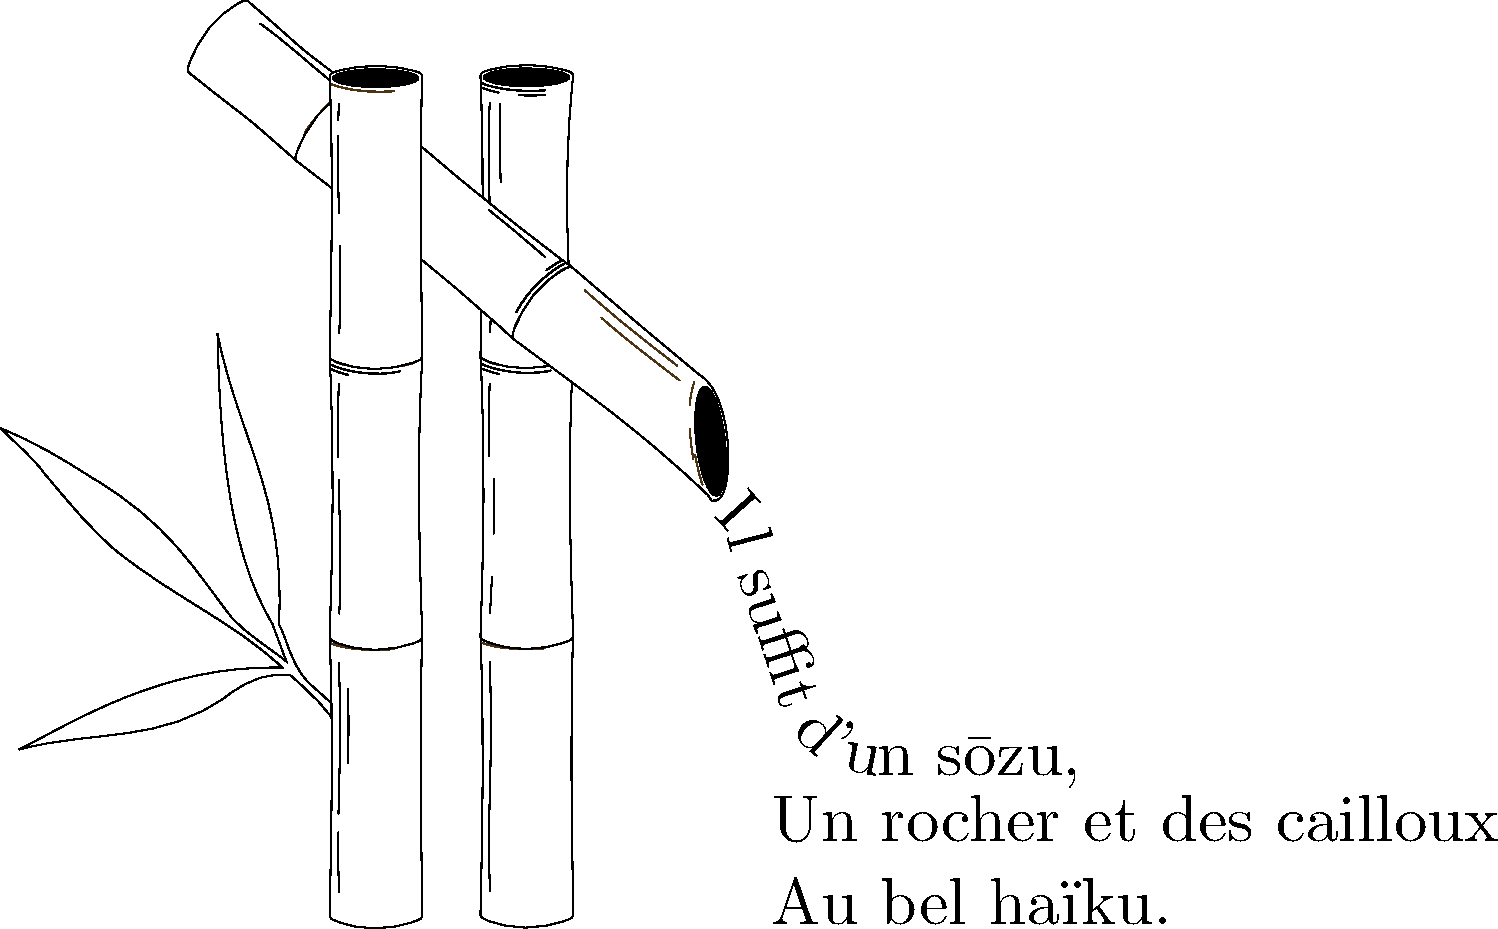
\includegraphics[width=7.5cm]{haiku.pdf}
  \index{Ecriture@Écriture}\index{Japon}
\end{floatpoem}

\poemtitle{Malin génie}\index{Humour}
%\setIndexNameEntry[]{}
\begin{verse}%
  \quatrain%
  \metric{11}\metric{10}%
  \rhyme{en}%
  \rhyme[e]{é}%
  Me demandais-je en me mirant longuement\\  % 
  Qui de moi ou de lui est le reflet,\\  % 
  Qui de nous deux vit dans la réalité\\  % 
  Quand l’autre me répondit \enquote{Ça dépend !}.
\end{verse}

\afterpage{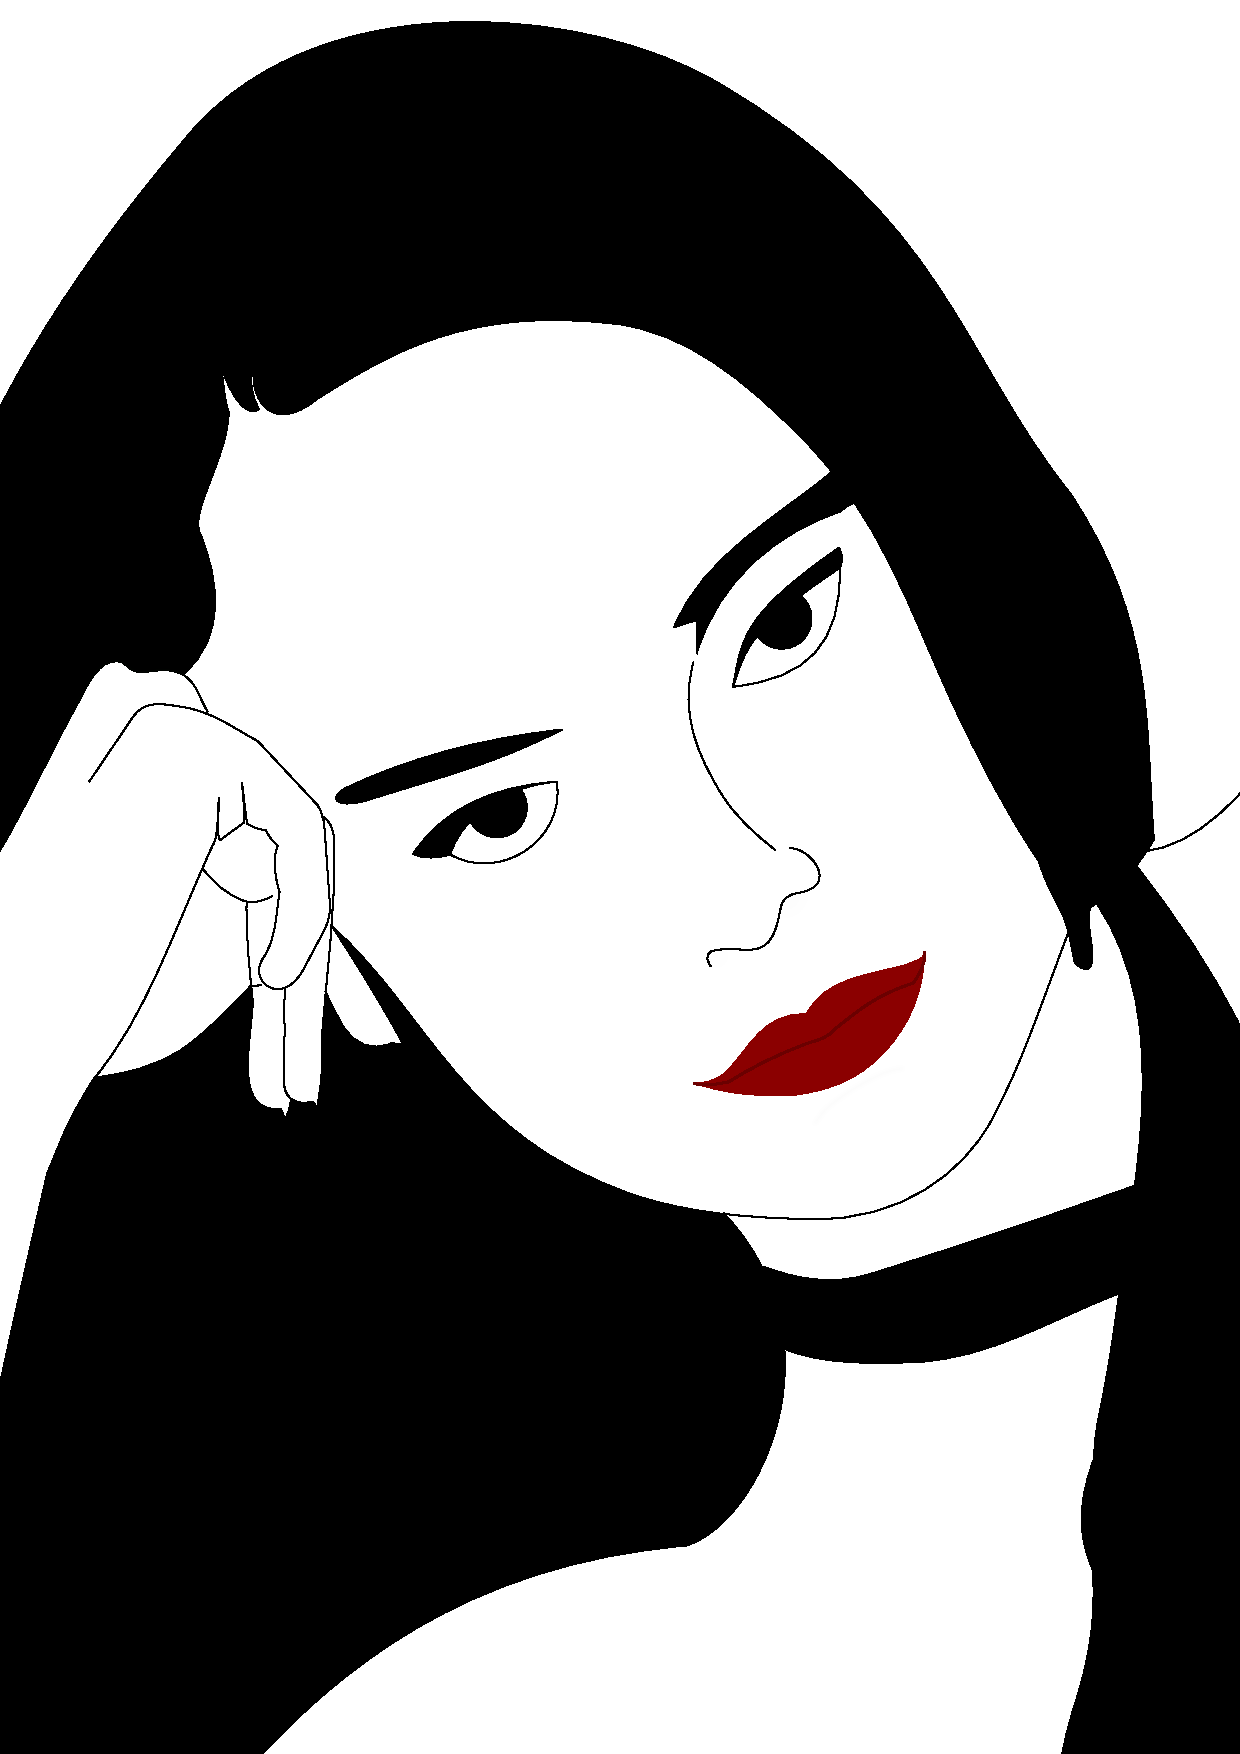
\includepdf[pages={1},addtolist={1,figure,{Mademoiselle F***** au sourcil encoché},encoche}]{portman-encoche.pdf}}
\section*{Trois odes de confinement, autant de quatrains, un zajal, une élégie, une complainte, et un haïku à F*****}
\markboth{}{Trois odes \& quat. zaj. élég. comp. haïk.}
\addcontentsline{toc}{section}{Trois odes de confinement, un zajal, deux quatrains, une élégie, une complainte, et un haïku à F*****}

\begin{prose}
  Je rencontrai alors mademoiselle F***** dont l’une des particularités qui me séduisit immédiatement est que la pointe de son sourcil gauche est encochée. Il y a tant de mystères dans ce sourcil encoché que j’en fus intrigué.

  Et comme alors je dessinais l’alphabet de Luca \textsc{di~Borgo} aux proportions du nombre d’or ; j’entrepris de suivre ses instructions de dessin et d’adapter les principes qui président à l’harmonie de ses lettres afin d’obtenir une variante de la lettre \autonym{F}, initiale de la demoiselle, dont l’attaque est encochée. 

%  Je suivis les instructions de \textsc{di~Borgo}, en adaptant les principes président à l’harmonie de ses lettres pour encocher l’attaque de l’\autonym{F}.
\end{prose}




\poemtitle{Tasse renversée}\index{Humour}
%\setIndexNameEntry[]{}
\begin{verse}%
  \quatrain%
  \metric{10}%
  \rhyme{qui}%
  \rhyme{i}%
% % Variente en tercet
%Ayant renversé ma tasse sur le tapis,\\  % 
%Je suis  plus déçu pour le contenu exquis :\\  % 
%Le précieux café  que je n’ai pas fini.
%
% Variente en quatrin
  Ayant renversé le liquide exquis,\index{Café}\\  % 
  Aussitôt affolé je m’en enquis\\  % 
  Bien moins soucieux du tapis sali\\  % 
  Que du café que je n’ai pas fini.
\end{verse}

\begin{figure}[h]
  \centering
  
\includegraphics[height=2cm]{F.pdf}
  \captionsetup{labelformat=empty}
  \caption[Lettre \autonym{F} à l’attaque encochée]{}
  \index{Ecriture@Écriture!Typographie}
\end{figure}



\begin{prose}
  Je m’en souvins tant et si bien qu’il me revint à l’esprit ce jour où, devant se préparer pour se rendre à un mariage, elle voulut se faire les sourcils.
%  J’ai souvenir que, pour se rendre à un mariage, elle voulut se faire les sourcils.

  Je lui suggérai alors de ne les refaire qu’à la condition de conserver cette encoche si singulière.
\end{prose}

\poemtitle[L’exhortation de Ȝumār par le sourcil fendu]{L’exhortation de \fallbackserif{\textbf{Ȝ}}umār\endnote{On rapporte que l’apôtre Ȝumār a annoncé \enquote{Apprenez à vos enfants l’archerie, la natation, et l’équitation}. Or, chaqu’une des trois premières strophes de ce poème s’attache à l’une de ces disciplines en constituant alors un triptyque.} par le sourcil fendu}%
\setIndexNameEntry[exhortation de umar par le sourcil fendu]{L’exhortation de Ȝumār par le sourcil fendu}
\renewcommand\currentpoemtitle{L’exhortation de \fallbackserif{\textbf{Ȝ}}umār par le sourcil fendu}%
\index{Islam}\index{Femmes!Yeux}\index{Amour}\index{Epique@Épique}
\begin{verse}%
  \quatrain%
  \metric{8}\metric{10}\metric{11}\metric{12}%
  \rhyme{ouble}%
  \rhyme[iere]{ière}%
  %
  \rhyme[an]{[a\textbar{}o]n}%
  \rhyme{age}%
  %
  \rhyme{eu}%
  \rhyme{ain}%
  %
  \rhyme{oir}%
  \rhyme{o}%
  %
  Le sourcil fendu à la pointe double\\
  Qui s’encoche à l’arcade sourcilière\\
  Que bande la mydriase singulière,\\
  Lorsqu’il prend mon regard pour cible, me trouble.\index{Archerie}

  Il me projette sur les eaux d’un océan,\index{Mer!Navigation}\\
  Là où ma brasse laisse deux longs sillons.\\
  Et cette nage haletante mais pélage%
  \endnote{Hapax dû à la licence poétique. De \autonym{pélagique}, \enquote{de haute mer}.}\\
  Me fait échoir épuisé sur le rivage

  Où la jument me fouette de sa queue\\\index{Chevaux}
  Qui, dans le vent, se scinde en deux.\\
  La chevauchant, Zulfixār\endnote{Épée à pointe double que Mahomet a trouvé dans le butin de la bataille de Badr.} en main,\index{Guerre!Epee@Épée}\\
  Elle m’entraîne au galop jusqu’au lointain.

  Mystère du défaut qui se fit victoire.\\
  Surlignant de l’encre l’iris \xenism{barroco}\endnote{Du portugais \xenism{barroco}, désigne en joaillerie une pierre belle parcequ’irrégulière.}\label{foot.barroco}\\
  Kintsungi\index{Japon}\endnote{Du japonais 金継ぎ \enquote{jointure d’or}, désigne une technique de céramique brisée dont en suite les morceaux sont rassemblés par une jointure d’or, lui conférant un plus bel aspect que si elle était intacte. À rapprocher de la note \ref{foot.barroco}.} rendit-il le mammaire ivoire\\
  Et mon cœur palpite sous les pectoraux.
\end{verse}

%\begin{figure}
%\centering
%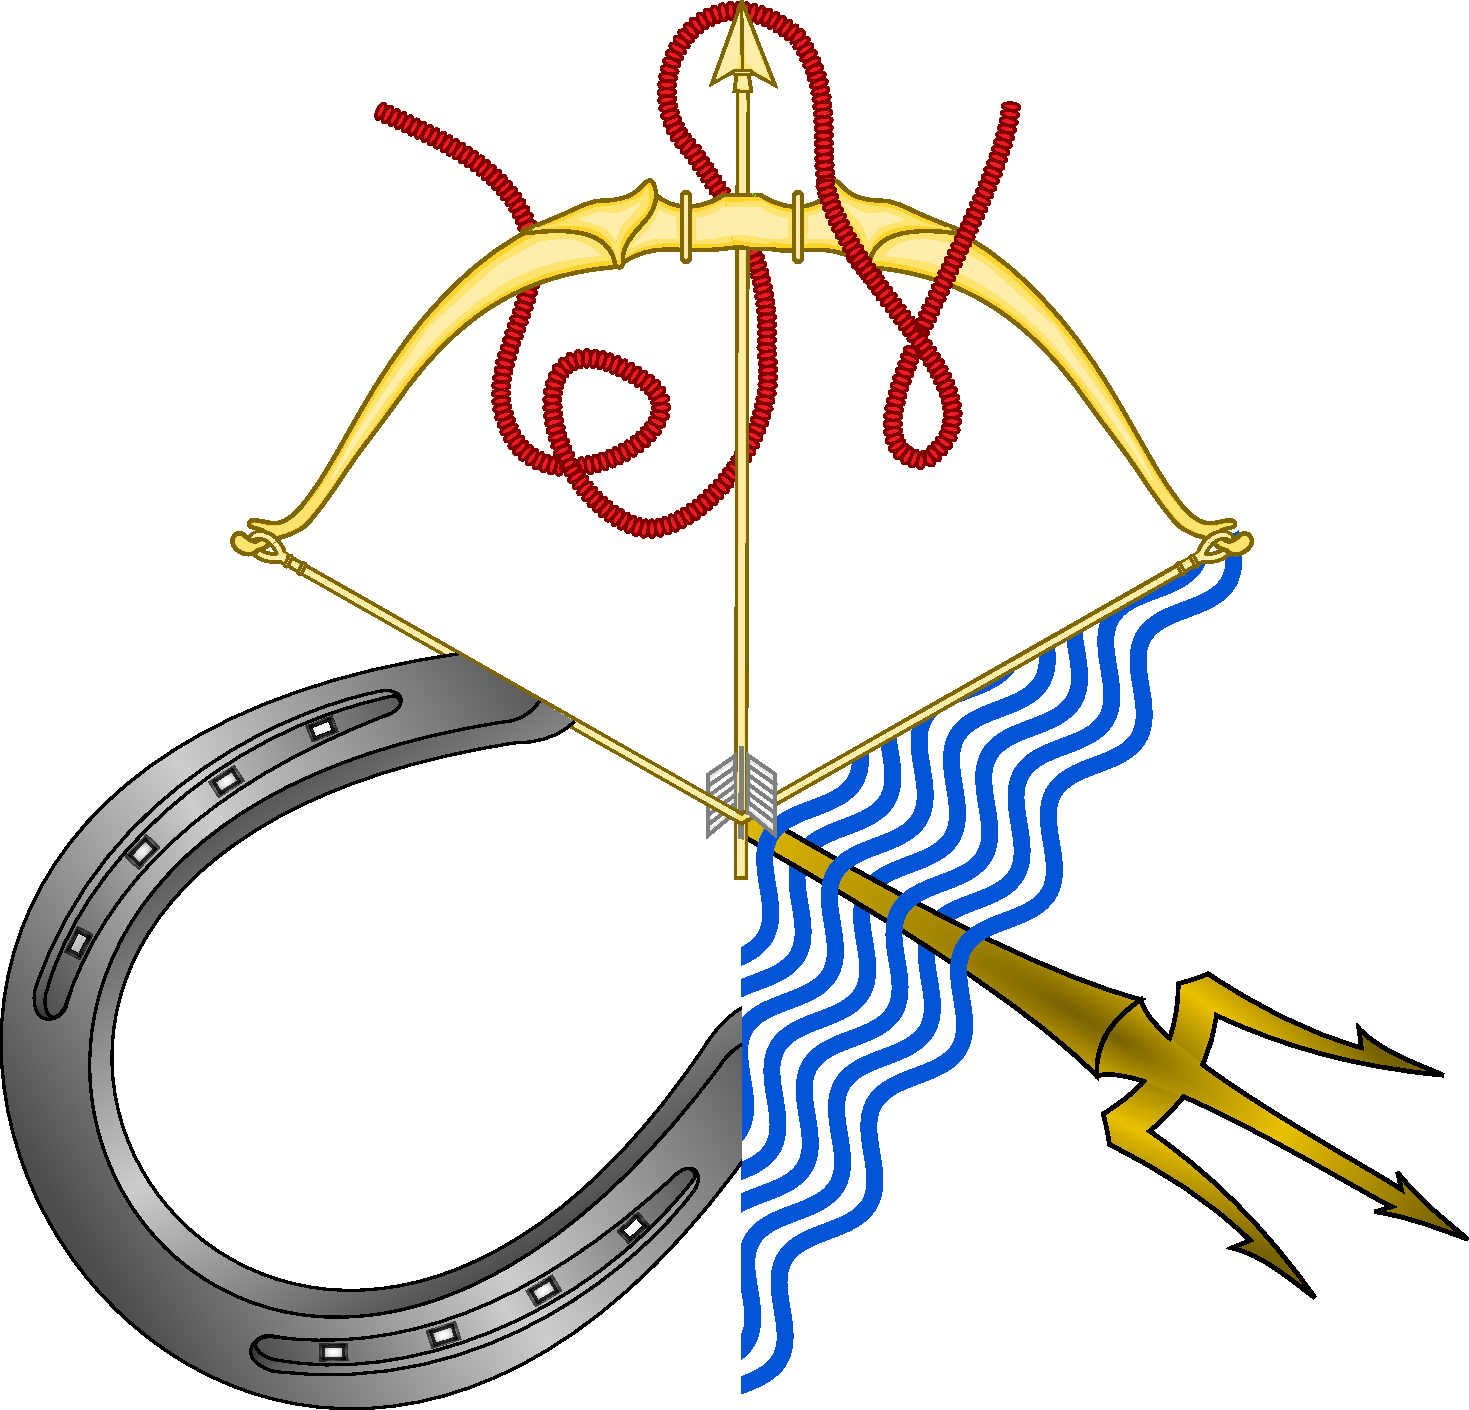
\includegraphics[width=0.70\textwidth]{tripaedie.pdf}
%\captionsetup{labelformat=empty}
%\caption[Tripaédie ou éducation par les trois disciplines]{}
%\end{figure}


\poemtitle{Un sourire et j’anhéle}\index{Femmes}
%\setIndexNameEntry[]{}
\begin{verse}%
  \quatrain%
  \metric{12}\metric{7}%
  \rhyme{ial}%
  \rhyme[acle]{acle}%
  \rhyme{an}%
  \rhyme[mon]{m[o\textbar{}e]n}%
  Elle projette les aurores radiales\\  % 
  Lorsque, retroussant le bourrelet labial,\\  % 
  Les commissures de ses lèvres se renâclent,\\  % 
  Poignardant de fougue mon thorax en débâcle.

  Ce sentiment haletant,\\  % 
  Aspire l’air ambiant,\\  % 
  L’engouffre dans les poumons,\\  % 
  Et l’expire promptement.
\end{verse}

\poemtitle{La faufilade sous le chemisier}\index{Femmes}
\setIndexNameEntry[faufilade sous le chemisier]{La faufilade sous le chemisier}
\begin{verse}%
  \quatrain%
  \metric{10}\metric{11}\metric{14}%
%  Souple est l’orbe voluptueux,\\  % 
%  Serti du rubis le plus précieux.\\  % 
%  Porté en avant, orgueilleux et galbé,\\  % 
%  Il est de la reine la fierté.
%
%  Tenu en main, son verni de velours\\  % 
%  Submerge de la languissante volupté\\  % 
%  Et s’en va alors fleurir et enfler\\  % 
%  Car de tendresse flatté à son tour.
%
%  Hallebardier est l’outremer chemisier,\\  % 
%  Celui aux pépites d’or parsemé,\\  % 
%  Sous lequel une herse sévère entrave,\\  % 
%  Avec de l’amante le regard grave.
%
%  Sur les tours cylindres, les assauts font défection\\  % 
%  Mais autour de l’imprenable citadelle sphérique,\\  % 
%  La belle rotondité accroit l’arduité mégalithique,\\  % 
%  Dont les attraits obstinent cependant l’assaillant.
%
%
  \rhyme{ieu}%
  \rhyme[e]{é}%
  \rhyme{our}%
  \rhyme[te]{té}%
  \rhyme[e]{é}%
  \rhyme{rave}%
  \rhyme[ian]{i[o\textbar{}a]n}%
  \rhyme{ic}%
  Ah, qu’il est souple  l’orbe voluptueux.\\
  Serti du rubis le plus précieux.\\
  Brandi en avant, orgueilleux et galbé,\\
  Il est de la reine la fierté.

  Même tenu en main, son verni de velours\\
  Submerge de la languissante volupté\\
  Et va fleurir et enfler à son tour\\
  Car de tendresse il est aussi flatté

  Hallebardier est l’outremer chemisier,\\
  Celui aux pépites d’or parsemé,\\
  Sous lequel une herse sévère entrave,\\
  Avec de l’amante le regard grave.

  Sur les tours cylindres\index{Guerre!Architecture militaire}\endnotemark[\getrefnumber{foot.tourRonde}], les assauts font défection\\
  Mais autour de l’imprenable citadelle sphérique,\\
  La rotondité accroît l’âpreté mégalithique,\\
  Dont tous les attraits obstinent cependant l’assaillant.
\end{verse}


\begin{prose}
  Le poème qui vient est écrit en maghrebi, le dialecte marocain, \caution{langue qui malgré son apparente ressemblance avec l’arabe littéral du fait de quantité de racines, tiendrait davantage du carthaginois}.

  Il aborde dans un style proche du genre musical chaabi \incise{que j’honni pourtant} des thèmes enracinés dans un tropisme marocain et sans doute même passéiste. Mais dont les préoccupations animent à s’y méprendre les contemporains.

  La traduction qui en est donnée, qu’après réflexions je voulu davantage littérale quoique s’accommodant de quelques adaptations plus littéraires, trahis forcément les rîmes et la métrique.
  J’avais pourtant fermement songé à rendre le texte maghrébi par un équivalent littéraire qui sacrifierais sans hésiter le sens pour ne conserver que l’exaltation qui en est ressentie. Choix auquel j’ai, sans doute à tort, fini par renoncer.
\end{prose}

\pagebreak
\begin{longtable}{R{0.3\textwidth} L{0.65\textwidth}}
  \noalign{%
    \vspace{-0.5cm}%
    \poemtitle[Zajal d’un insomniaque épris — \textarabic{زجل العشّاق الصهران}]{\textarabic{زجل العشّاق الصهران} — Zajal d’un insomniaque épris}%
    %\renewcommand\currentpoemtitle{Zajal d’un insomniaque épris}%
    \setIndexNameEntry[Zajal dun insomniaque épris]{Zajal d’un insomniaque épris}
    \distique%
    }
  \endfirsthead

  %\vspace{0.35cm}

  \textarabic{أنا بالليل}                  &       Dans mes nuits\index{Nuit},   \\  % 
  \textarabic{حاضي الگمرا لا تطير.}         &       Je veille à ce que la lune ne croule\index{Astronomie}.   \bigskip \\ 
  \textarabic{ضال فايق،}                   &       Demeurant éveillé\index{Insomnie},   \\  % 
  \textarabic{و فبالي صوت الضقايق،}        &       L’esprit des percutions de cuivre imbibé\index{Musique},   \bigskip \\ 
  \textarabic{راني خايف}                   &       Je crains   \\  % 
  \textarabic{لَي جي يقجني السّالف.}         &       Que la longue\index{Femmes!Cheveux} natte vienne m’étrangler.   \bigskip \\ 
  \textarabic{و معا الغربي،}               &       Et avec le zéphyr,   \\  % 
  \textarabic{يطيّر ما باقى دنعاسي.}        &       Sera ravi ce qui me reste de sommeil.   \bigskip \\ 
  \textarabic{نفكّر فالغزال}                &       Je songe à la belle\index{Femmes}   \\  % 
  \textarabic{لي گع ميخطى البال.}          &       Qui ne quitte jamais mes pensées.   \bigskip \\ 
  \textarabic{منفخا عليىا}                 &       Me dédaignant,   \\  % 
  \textarabic{و متخصر حتا شوفى فيا.}       &       Elle ne m’accorde pas un seul regard.\index{Femmes!Yeux}   \bigskip \\ 
  \textarabic{ورى الشبيك}                  &       À travers le moucharabieh   \\  % 
  \textarabic{ما تورّي لجيهتي غير الشيك}    &       Elle ne me laisse paraitre que la superbe   \bigskip \\ 
  \textarabic{وخى هكّاك،}                   &       Et malgré tout,   \\  % 
  \textarabic{من الشريكة متبوس الحناك.}    &       De la rivale elle ne daigne embrasser les joues.   \bigskip \\ 
  \textarabic{مولات التاج}                  &       En dépositaire de la couronne,   \\  % 
  \textarabic{إلى سمعات غيرها تعواج.}      &       Si elle vient à entendre parler d’une autre qu’elle, se contrarie.   \bigskip \\ 
  \textarabic{گع النهار،}                  &       Toute la journée,   \\  % 
  \textarabic{منها ما نشوف غير الضهر.}     &       Je ne perçois d’elle que le dos.   \bigskip \\ 
  \textarabic{بكترت ما جميل}               &       Par tant de beauté,   \\  % 
  \textarabic{شعرها الكحل غلب الليل}       &       Ses cheveux noirs vainquent la nuit.   \bigskip \\ 
  \textarabic{طول من النّيل}                &       Plus long que le Nil,\index{Egypte@Égypte!Nil}   \\  % 
  \textarabic{و ضلامو يطفي الپيل.}          &       Son obscurité éteint la lampe-torche.   \bigskip \\ 
  \textarabic{الگمرا ولات فطحا}             &       La lune parait plate  \\  % 
  \textarabic{فگلستها الماّحا.}             &       À l’avènement de son assise raffinée.   \bigskip \\ 
  \textarabic{الزيف \xenism{الريض} (الحمر)}         &       Si le voile \xenism{red} (rouge)   \\  % 
  \textarabic{الا مشا حتا زلق نفيض.}        &       Vient à glisser, je fond.   \bigskip \\ 
  \textarabic{لعندي،}                      &       Vers moi,   \\  % 
  \textarabic{راهى حالفا ربي لا تجي.}       &       Elle jure par Dieu de ne jamais venir.   \bigskip \\ 
  \textarabic{بلا كوڤيد}                    &       Sans covid,   \\  % 
  \textarabic{فراقها خلاني مريض.}            &       La séparation me laisse malade. \bigskip \\ 
  \textarabic{معا ليالي،}                  &       Avec mes nuits,   \\  % 
  \textarabic{دّات لي حتى قلبي.}            &       Elle a emporté jusqu’à mon cœur.   \bigskip \\ 
  \textarabic{تا من العقل}                 &       Et mon encéphale aussi   \\  % 
  \textarabic{ولّا كي الآلة فالمعمل.}        &       Est devenu tel l’engin de l’usine.   \bigskip \\ 
  \textarabic{يضل يخدم}                    &       Il demeure en fonction   \\  % 
  \textarabic{ميمشي منو الهمّ.}             &       Et ne se défait de l’anxiété.   \bigskip \\ 
  \textarabic{شغادي يصنع}                  &       Qu’escompte produire   \\  % 
  \textarabic{لي حتا امّ الربيع ميقطع؟}     &       Celui qui ne traverse le fleuve d’Um~al~rabiȝ\endnote{Fleuve usuelement graphié \autonym{Oum Errabiâ} prenant sa source aux environs de Khénifra  et débouchant vers les environs d’Azemmour dans l’océan Atlantique. De ce fait, un voyageur qui irait de Kénitra à Eljadida, le traverserait.}\,?   \bigskip \\ 
  \textarabic{لي بغي يزيد}                 &       Celui qui s’avance   \\  % 
  \textarabic{من مهديه لسيدي بوزيد}        &       De Mehdia vers Sidi~Bouzid\endnote{Communes respectivement proches de Kénitra et d’Eljadida.} \bigskip \\ 
  \textarabic{يبقى يتجّر}                   &       Demeure entrainé   \\  % 
  \textarabic{فاليل حتى يودّن الفجر.}       &       Dans la nuit jusqu’à ce que retentisse  l’aurore\endnote{Le texte marocain utilise le mot \textarabic{فجر} (\xenism{fajr}) soit une allusion à la prière de l’aurore. D’où le retentissement dû à l’\xenism{āḋān}.}.   \bigskip \\ 
  \textarabic{ربي العالي}                  &       Grand Dieu,   \\  % 
  \textarabic{بغيت منها غير الشفاري}       &       Je n’espère d’elle que (voir) les paupières   \bigskip \\ 
  \textarabic{و إلى ما لقيتها}             &       Et si je ne la trouve pas,   \\  % 
  \textarabic{نضلّ نقلّب على القافية.}       &       Je poursuivrais la recherche des rîmes.\index{Propos réflexif}   \\  % 
\end{longtable}

\poemtitle{La voir dans la nuit}
%\setIndexNameEntry[]{}
\begin{verse}%
  \quatrain%
  \metric{10}%
  \rhyme{i}%
  \rhyme{eu}%
  L’ardeur qui me pousse à l’admirer malgré la nuit\index{Nuit}\index{Femmes}\\  % 
  Contraint ma perception à la nyctalopie,\\  % 
  Si bien qu’en son absence tout parait odieux\\  % 
  Et y est préférable de se crever les yeux.
\end{verse}

\poemtitle{À distance}
\setIndexNameEntry[a distance]{À distance}
\begin{verse}%
  \quatrain%
  \metric{11}%
  \rhyme[an]{[a\textbar{}o]n}%
  \rhyme{fil}%
  Un amour que peut-être nous tisserons\\  % 
  Par delà les montagnes et océans\\  % 
  Avec l’RJ45\endnote{Le nom usuel quoique fautif d’RJ45 désigne les cables 8P8C sérvant à connecter des machines à un réseau Ethernet et plus généralement à l’Internet.} pour fil\index{Technique}\\  % 
  Mais le chas est trop étroit pour qu’on l’enfile.
\end{verse}

\begin{prose}
  Dans un café\index{Café!Etablissement cafe@Établissement café}, j’attendais F***** ou même un signe de sa part, un appel téléphonique, un message. Tandis que le temps passait, des noix de palmiers tombaient à intervalle plus ou moins régulier, comme pour ponctuer le défilement du temps.
\end{prose}

\poemtitle{L’absence}
\setIndexNameEntry[absence]{L’absence}
\begin{verse}%
  \monostique\quatrain%
  \metric{6}\metric{7}\metric{8}\metric{9}\metric{10}
  \rhyme[e]{é}%
  %
  \rhyme{indre}%
  \rhyme{verse}%
  %
  \rhyme[er]{ère}%
  \rhyme{fer}%
  \rhyme[e]{é}%
  %
  \rhyme{oi}%
  \rhyme{ense}%
  %
  \rhyme{role}%
  \rhyme[e]{é}%
  Gorgée après gorgée,\\  % 
  Mon verre s’est vidé.\index{Café}\\  % 
  Et l’anse ne saurait,\\  % 
  À tes bras, suppléer.
%Et l’anse ne saura\\  % 
%tes bras substituer\\  % 

  \emph{Ô yeux, ô nuit, ô nuit, ô yeux.}

  Ô voix de plus en plus moindre\\  % 
  Qui tombe comme l’averse\index{Eau}\\  % 
  Mais qui ne saurait éteindre\\  % 
  Le brasier\index{Feu} qui me traverse.

  \emph{Ô nuit, ô yeux, ô nuit, ô yeux.}

  Maudit instant où, de mon verre,\\  % 
  N’apparaît que fin liseré\\  % 
  Où subsiste peu de café.\\  % 
  J’ignore en vérité qu’en faire.\\  % 
  Assurément qu’à l’achever\\  % 
  Je me résoudrais que par fer.

  \emph{Ô yeux, ô nuit, ô yeux, ô nuit.}

  Le palmier qui laisse échoir ses noix,\\  % 
  Dont la pourtant sévère  cadence\\  % 
  Rappelle ta si pénible absence,\\  % 
  Pleure à mes cotés mon désarrois.

  \emph{Ô nuit, ô nuit, ô yeux, ô yeux.}

  Lorsqu’avec grande flagrance, ton rôle\\  % 
  Dissone d’avec tes rares paroles\\  % 
  Pour quels choix, dis-moi, puis-je encore opter\\  % 
  Tandis que tu ne veux t’en expliquer ?

  \emph{Ô nuit, ô yeux, ô yeux, ô nuit.}

  Concède et pardonne\\  % 
  Qu’aux yeux me fixant\index{Femmes!Yeux}\\  % 
  Gorgés d’océans\\  % 
  Je m’abandonne.
  %
  \rhyme{done}%
  \rhyme{an}%
  %
  \rhyme{a}%
  \rhyme{our}%

  \emph{Ô yeux, ô nuit, ô nuit, ô yeux.}

  Toi qui ailleurs dirige le mât,\index{Mer!Navigation}\\  % 
  En fait de tout louvoyant discours,\\  % 
  Si tu dubites de mon amour,\index{Amour}\\  % 
  Regarde ma vulve et tu saura\index{Femmes}.
\end{verse}

\poemtitle{Du naufrage}\index{Mer!Navigation}\index{Epique@Épique}
\setIndexNameEntry[naufrage]{Du naufrage}
\begin{verse}%
  \haiku
  \rhyme[e]{é}%
  J’ai perdu ma proue\\  % 
  Et mon navire a coulé,\\  % 
  Dans l’eau, tout entier.
\end{verse}

\begin{figure}[h]
  \centering
  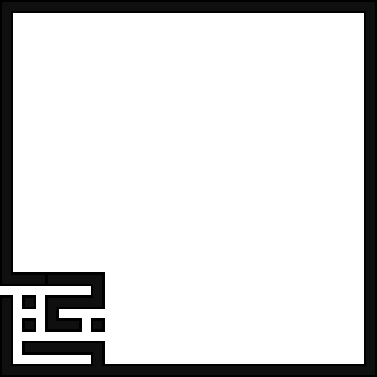
\includegraphics[width=0.9\textwidth]{farir.pdf}
  \captionsetup{labelformat=empty}
  \caption[Idéotexte du \autonym{vide} (\textarabic{خالي})]{}
\end{figure}

\begin{prose}
  Me trouvant non loin du musée de la banque centrale du Maroc, je me dis qu’il valait encore mieux y noyer ma peine. Grand bien me pris car alors \incise{joi} bien loin de m’en douter, j’y trouvais des éléments prélevés sur le site archéologique d’Aghmat, des parties de la maison d’Al\,Mutamid ibn~Abbad\index{Personnages historiques!Al\,Mutamid ibn~Abbad} qui commandita à Lissān~al\,Ḋḋīne ibn~al\,Xatīb\index{Al\,Andalous!Lissān~al\,Ḋḋīn ibn~al\,Xatīb} des poèmes à graver sur ses murs. Mais plus bouleversant encore, un manuscrit que je crus comprendre autographe de Lissān~al\,Ḋḋīne ! Fort heureusement, le masque que je portais du fait de l’épidémie m’épargna le ridicule d’exposer aux gens les larmes qui coulèrent le long de mes joues. Je me suis même retenu de m’assoir par terre tant mes jambes s’étaient vidées de leur tonus.

  Je dois toute fois être honnête, je n’ai pas pris la peine de vérifier que les manuscrits étaient bien autographes comme j’ai cru le comprendre ; ou plus exactement j’ai soigneusement évité de m’en assurer, préférant me complaire dans l’idée qu’ils l’étaient.
\end{prose}

\poemtitle[Le Zurbiy]{Le \xenism{Zurbiy}\endnote{Le dernier sultan de Grenade, Mohammed XII de Grenade, dit al\,Zurbiy \xenism{l’infortuné} fut le dernier souverain musulman d’al\,Andalous.}}\index{Al\,Andalous!Reconquista}
%\setIndexNameEntry[]{}
%\renewcommand\currentpoemtitle{Le Zurbiy}%
\setIndexNameEntry[Zurbiy]{Le Zurbiy}
\begin{verse}%
  \quatrain%
  \metric{11}\metric{8}\metric{10}%
  \rhyme{i}%
  \rhyme{mat}%
  \rhyme{zir}%
  \rhyme{teur}%
  Comme un prince de son royaume banni,\\  % 
  Qui ne reverra plus  son Andalousie,\\  % 
  De notre amour\index{Amour}, l’échec et mat\\  % 
  M’est aussi odieux qu’Aghmat.\endnote{Al\,Mutamid Ibn~Abbad  qui a été roi de Séville, fût destitué par les Almoravides pour être exilé à Aghmat où il mouru.}

  Que vienne me voir le Double-Visir\endnote{Allusion à Lissān~al\,Ḋḋīne ibn~al\,Xatīb, savant qui fut par deux fois ministre aux cours nasride et mérinide, ce qui lui valut le surnom de \enquote{celui aux deux visirat} \textarabic{ذي الوزارتين}. Lors de son exil à Aghmat, Al\,Mutamid Ibn~Abbad fit appel à ses services de poète pour rédiger des vers qui furent calligraphiés sur les murs de sa maison.}\\  % 
  Et qu’avec ses royaux vers enchanteurs,\\  % 
  Ceux qui sont gravés loin sur les hauteurs,\index{Ecriture@Écriture!Epigraphie@Épigraphie}\\  % 
  Soit marquée l’extinction du désir.
\end{verse}

\section*{Kénitra}
\markboth{}{Kénitra}
\addcontentsline{toc}{section}{Kénitra}

\poemtitle{Matin}
%\setIndexNameEntry[]{}
\begin{verse}%
  \quatrain%
  \metric{12}%
  \rhyme{iar}%
  \rhyme{in}%
  Luisants sous quelques néons à l’éclat criard\index{Synthwave}\\  % 
  Dans la ville engourdie où larmoie le brouillard,\\  % 
  Les rideaux encore baissés des magasins\\  % 
  Sont aussi lourds que les paupières le matin.
\end{verse}

\poemtitle{L’étudiante du matin }\index{Femmes}
\setIndexNameEntry[etudiante du matin]{L’étudiante du matin}
\begin{verse}%
  \sizain%
  \metric{11}%
  \rhyme[ute]{uté}%
  \rhyme{heur}%
  \rhyme{ter}%
  Pour voir les lueurs du jour qui débutait,\\  % 
  Je m’étais levé le matin de bonheur\\  % 
  Où le premier rayon ayant touché terre\\  % 
  Me demanda où était la faculté.\\  % 
  Ah, que ne lui aurais-je fais cours sur l’heure\\  % 
  Si j’avais eu un grade universitaire.
\end{verse}

\begin{prose}
  Je prononçais le quatrain suivant un matin de janvier dans un café où je me retrouvais avec une amie  qui, en se coiffant, s’en révélera être la muse.
\end{prose}

\poemtitle{La crinière}\index{Femmes!Cheveux}
\setIndexNameEntry[criniere]{La crinière}
\begin{verse}%
  \sizain%
  \metric{10}\metric{11}%
  \rhyme[cheve]{chev[o\textbar{}e]}%
  \rhyme[iere]{ière}%
  Elle tenait dans sa bouche ses cheveux\\  % 
  Tandis qu’elle se peignait la crinière\\  % 
  Comme l’on fait tenir le mord aux chevaux\\  % 
  Et moi, je la regardais sans œillères.
\end{verse}

\begin{prose}
  Si heureux de l’avoir composé, j’ouvris mon journal et tout le monde me vit esquisser un large sourire de satisfaction en lisant un article intitulé \work{Armes françaises pour dictature exemplaire}.
\end{prose}

\poemtitle{Du soleil dans mon café}\index{Astronomie!Soleil}\index{Café}
%\setIndexNameEntry[]{}
\begin{verse}%
  \sizain%
  \metric{7}\metric{7}%
  \rhyme[eye]{èye}%
  \rhyme{on}%
  Instant sans pareil\\  % 
  Que celui où le soleil\\  % 
  Pointe son premier rayon\\  % 
  Sur mon guéridon.
\end{verse}

\poemtitle{Le vert talus}
\setIndexNameEntry[vert talus]{Le vert talus}
\begin{verse}%
  \quatrain%
  \metric{9}\metric{8}%
  \rhyme{alu}%
  \rhyme[asse]{assé}%
  Accompagne-moi au vert talus.\\  % 
  Je t’en prie, viens t’y prélasser.\\  % 
  Tu y trouveras le salut\\  % 
  Dans lequel tu pourras rêvasser.
\end{verse}

\poemtitle{Le regard bleu}\index{Femmes!Yeux}
\setIndexNameEntry[regard bleu]{Le regard bleu}
\begin{verse}%
  \quatrain%
  \metric{11}%
  \rhyme{troi}%
  \rhyme[entimen]{[e\textbar{}o]ntimen}%
  Devant son regard bleu où s’ouvre un détroit\index{Mer!Navigation}\\  % 
  Celui qui en séparant deux continents,\\  % 
  Éloigne les nefs achéennes de Troie,\index{Mythologie grecque!Troie}\\  % 
  Comment n’éprouverais-je aucun sentiment ?
\end{verse}

\poemtitle{Collision}\index{Epique@Épique}
%\setIndexNameEntry[]{}
\begin{verse}%
  \quatrain%
  \metric{10}%
  \rhyme[ete]{ète}%
  \rhyme[ere]{ère}%
  \rhyme{a}%
  \rhyme[verse]{versé}%
  Flottant dans la flaque d’eau violette\index{Synthwave}\index{Eau},\\  % 
  Les jets de lumière des lampadaires\\  % 
  Vinrent s’éclabousser sur mes lunettes\\  % 
  Quand t’arrives dessus en roue arrière.

  Tu es passée à moto devant moi,\\  % 
  Et si tu as failli me renverser,\\  % 
  J’ai tout de même scandé un verset\\  % 
  Car je suis mort quand tu me regardas.\index{Femmes!Yeux}
\end{verse}

\poemtitle{Réminiscence de l’infante du Portugal}
\setIndexNameEntry[Reminiscence de l’infante du Portugal]{Réminiscence de l’infante du Portugal}
\begin{verse}%
  \haiku
  \rhyme{ade}%
  Ces yeux de saudade\\  % 
  Où se déploient les Cyclades\index{Mer}\\  % 
  Me font une œillade.\index{Femmes!Yeux}
\end{verse}

\begin{figure}[h]
  \centering
  
\includegraphics[width=\textwidth]{img/ines-syntwave.pdf}
  \captionsetup{labelformat=empty}
  \caption[Portrait synthwave d’Inèss]{}
  \index{Synthwave}
\end{figure}

\begin{prose}
  Je passais avec Inèss une de ces journées dont on parlera encore dans les siècles des siècles. Ne vous ai-je jamais parlé d’elle ? Nul besoin, l’ensemble de l’ouvrage est teinté de son emprunte.

  C’était une journée de juillet, c’en était la dernière. Je la passais avec la ravissante Inès. Et c’était comme un verre de café\index{Café} vide que l’on penche espérant ne rien gaspiller des ultimes gouttes qu’il peut peut-être encore contenir, ou s’il n’en reste pas, se faire croire que l’on a pu tout de même en grappiller.
  Quelle ne fut pas notre surprise, lorsque le mois de juillet s’avéra magicien car son verre avait un fond caché !

  D’autant que, et vous pourrez imaginer à quel point nous étions enjoués, Inès venait tout juste d’acquérir une automobile pour la première fois. C’était un prélude au mois d’août.

  Nous étions au 2021 juillet 31 et, tandis que fendaient sur nous les rayons crépusculaires, nous prenions la route, lunettes de soleil au museau en écoutant de la synthwave.
\end{prose}

\poemtitle{Virée d’avant août}
%\setIndexNameEntry[]{}
\begin{verse}%
  \quatrain%
  \metric{10}%
  \rhyme{ma}%
  \rhyme{on}%
  \rhyme{afe}%
  \rhyme[eye]{èye}%
  Toi et moi, sur l’écran de cinéma\index{Cinéma}\index{Synthwave},\\  % 
  Nous roulons droit devant vers l’horizon,\\  % 
  Vers tous nos rêves et nos passions\\  % 
  Loin de la sombreur du pont de l’Alma.

  Je veux capturer comme un photographe\index{Photographie}\\  % 
  L’instant précis où tu secoues ta coiffe\\  % 
  Éclabousse par les mèches rebelles,\index{Femmes!Cheveux}\\  % 
  Les reflets des lunettes de soleil.\index{Astronomie!Soleil}
\end{verse}

\begin{prose}
  Le lendemain, toujours en voiture évidement, nous partîmes nous baigner à l’embouchure du fleuve Sebou. Nous grimpâmes  sur les rochers de l’une de ses deux immenses jetées, enjambant les creux, cherchant les chemins les moins escarpés, pour finalement parvenir à un récif. Après nous être baignés, nous immergeâmes d’entre les vagues et les roches pour aller nous assoir sur un écueil à fleur d’eau. Et tandis que le ressac des vagues sur le rocher qui se faisait plus violent sonnait comme une caresse, Inès me demanda \enquote{Y a-t-il plus heureux que nous dans le monde à cet instant ?}. Qu’avais-je besoin de  répondre lorsque les vagues éteintes trouvaient encore le prolongement de leur éclat autant que de notre enchantement dans l’écume ?
%Là, nous nous baignâmes parmi les roches à fleur d’eau et les écueils.
\end{prose}

\poemtitle{Baignade avec Inès}\index{Mer}
%\setIndexNameEntry[]{}
\begin{verse}%
  \quatrain%
  \metric{11}\metric{10}%
  \rhyme{aze}%
  \rhyme{i}%
  \rhyme[ele]{èle}%
  \rhyme{o}%
  Caressée par les vaguelettes turquoises,\\  % 
  Est-ce l’eau qui la baigneuse a embellie\\  % 
  Ou est-ce sa beauté qui y déteignit,\\  % 
  Tant la mer devint diamant et topaze ?

  Je compris pourquoi la mer est si belle.\\  % 
  Souvenez-vous qu’au contact de sa peau,\\  % 
  L’éclat d’Inès y laissa des séquelles,\\  % 
  À chaque fois que vous boirez de son eau.
\end{verse}

\begin{prose}
  Encore à Kénitra où j’allais me faire injecter ma première dose de vaccin, je vis en  chemin une jeune femme qui m’inspirait. Et déjà j’imaginais mes amis à qui je raconterait la scène qui me railleraient, me demandant si toutes les passantes m’inspiraient. Commençant à composer une réponse à cette question imaginaire, je me disais \enquote{Ne mérite-t-elle pas un poème ?}.

  Je réfléchis alors à une  suite sans me douter qu’elle viendrait d’elle même lorsque je me serais rendu compte de ne pas être le seul à observer cette passante.
\end{prose}

\poemtitle{La muse}\index{Femmes}\index{Propos réflexif}\index{Humour}
\setIndexNameEntry[muse]{La muse}
\begin{verse}%
  \quatrain%
  \metric{10}%
  \rhyme[eme]{ème}%
  \rhyme{iste}%
  Ne mérite-t-elle pas un poème ?\\  % 
  \enquote{Si, bien sûr que si !} clamait le cycliste\\  % 
  Quand, la regardant le visage blême,\\  % 
  Le fourgon le renversa sur la piste.
\end{verse}


\poemtitle{Le bien inspiré}\index{Femmes}\index{Ecriture@Écriture}\index{Propos réflexif}
\setIndexNameEntry[bien inspiré]{Le bien inspiré}
\begin{verse}%
  \quatrain%
  \metric{10}%
  \rhyme[ame]{a[r]me}%
  \rhyme{rine}%
  L’on dit que j’écris au sujet des femmes,\\  % 
  Mais rien n’est plus faux, je ne suis que l’arme,\\  % 
  Quand elles me trempent dans la cyprine\\  % 
  Et me font transcrire l’humeur chagrine.
\end{verse}

\poemtitle{Torche}
%\setIndexNameEntry[]{}
\begin{verse}%
  \quatrain%
  \metric{12}%
  \rhyme[roche]{[r$\leftrightarrow$o]che}%
  \rhyme{main}%
  Les flammes\index{Feu} de cheveux\index{Femmes!Cheveux} voltigeant au vent proche,\\  % 
  Ce n’était pas une femme mais une torche.\\  % 
  Si sa taille semble se caler dans la main\\  % 
  Je la saisirais pour éclairer mon chemin.
\end{verse}

\poemtitle{Déception}
\setIndexNameEntry[Deception]{Déception}
\begin{verse}%
  \quatrain%
  \metric{8}%
  \rhyme{a}%
  \rhyme{aye}%
  \rhyme[an]{[a\textbar{}e]n}%
  Quelque chose en moi se brisa\\  % 
  Pourtant, rien n’eut lieu ce jour là.\\  % 
  Certes, pas grand chose en tout cas,\\  % 
  Quoique ce fut beaucoup pour moi.

  Un détail, un foutu détail.\\  % 
  De ceux qui sont déterminants,\\  % 
  Ceux qui sonnent comme une faille,\\  % 
  Qui s’annoncent fatalement.
\end{verse}

\poemtitle{Sentence}
%\setIndexNameEntry[]{}
\begin{verse}%
  \quatrain%
  \metric{8}%
  \rhyme{gar}%
  \rhyme{ine}%
  Je succombai à son regard\index{Femmes!Yeux}\\
  Dont les paupières assassines\\
  Qui de leur battement m’égarent\\
  Tombent comme des guillotines.
\end{verse}

\poemtitle{Cosmopolite}
%\setIndexNameEntry[]{}
\begin{verse}%
  \quatrain%
  \metric{9}%
  \rhyme{mosse}%
  \rhyme{u}%
  J’ai arpenté Doura-Europos\\  % 
  Et ai sillonné ses avenues.\\  % 
  C’est alors ma cité que j’ai vu\\  % 
  Car je suis citoyen du cosmos.
\end{verse}

\poemtitle{Colère}
%\setIndexNameEntry[]{}
\begin{verse}%
  \quatrain%
  \metric{9}%
  \rhyme{gar}%
  \rhyme{men}%
  \rhyme{aine}%
  \rhyme[an]{[a\textbar{}e]n}%
  Pour les dérober aux maints regards,\\  % 
  Il enfouit ses ressentiments\\  % 
  Là, sous des profondeurs souterraines\\  % 
  Si vastes que de leur déblaiement\\  % 
  Émergea un tertre trop voyant,\\  % 
  Qui inscrivit les traits de la haine\\  % 
  Sur son visage blême et hagard.
\end{verse}



\poemtitle{Le surfléché}\index{Archerie}
\setIndexNameEntry[surfleché]{Le surfléché}
\begin{verse}%
  \quatrain%
  \metric{12}%
  \rhyme[e]{é}%
  Comme un soldat tombé au sol car sur-fléché\\  % 
  Qui scrute le champs d’honneur avant d’abdiquer\index{Guerre!Bataille}\\  % 
  Et sur lequel pleuvent les flèches acérées,\\  % 
  Je suis assailli de ses  baisers enflammés.\index{Amour}
\end{verse}

\poemtitle[Le nay]{Le nay\endnote{Flûte à l’origine perse d’où elle tire son nom signifiant \autonym{roseau}, mais aussi turque et arabe intervenant en général dans le répertoire de la musique savante.}}\index{Musique}%
\setIndexNameEntry[nay]{Le nay}
\renewcommand\currentpoemtitle{Le nay}%
\begin{verse}%
  \quatrain%
  \metric{10}\metric{11}%
  \rhyme{ssonnay}%
  \rhyme[ame]{a[r]me}%
  Que le musicien prenne son nay,\\  % 
  Qu’il en insuffle l’air sacré dans nos âmes,\\  % 
  L’air qui apaise et fait déposer les armes\index{Guerre!Paix}\\  % 
  Et qu’avec, les turpitudes s’en aillent.
\end{verse}

\poemtitle{Sac de la bibliothèque d’Alexandrie}\index{Histoire!Antiquité}
%\setIndexNameEntry[]{}
\begin{verse}%
  \quatrain%
  \metric{11}%
  \rhyme{ivre}%
  \rhyme{vide}%
  Tel l’aveugle qui me toise en étant ivre\\  % 
  Et me regarde alors de ses globes vides,\\  % 
  La bibliothèque dégarnies de livres\\  % 
  Est un paysage insipide et livide.
\end{verse}

\poemtitle{Appelle-moi}\index{Urbanité}\index{Femmes}
%\setIndexNameEntry[]{}
\begin{verse}%
  \quatrain%
  \metric{9}%
  \rhyme{oir}%
  \rhyme{e}%
  %
  \rhyme{eur}%
  \rhyme{i}%
  %
  \rhyme{ture}%
  \rhyme{a}%
  %
  \rhyme{soir}%
  \rhyme{main}%
  %
  \rhyme{oir}%
  \rhyme[e]{é}%
  %
  \rhyme{a}%
  Khadija, appelle-moi ce soir\\  % 
  Et nous braverons le couvre-feu\\  % 
  Dans la nuit qui dérobe aux regards\\  % 
  L’ardeur de nos jeux facétieux.

  Les rideaux tombent, il est neuf heure.\index{Nuit}\\  % 
  Angle Mohamed~\textsc{v}—Diouri,\\  % 
  Viens y en ramenant des souchis\\  % 
  Et j’apporterais ma bonne humeur.

  Khadija, viens me voir en voiture,\\  % 
  Et nous prendrons d’asseau Kénitra\\  % 
  Qui pour nous sera des rues de Troie\index{Mythologie grecque!Troie}\\  % 
  Où nous deux courrons vers l’aventure.

  Khadija, appelle-moi ce soir\\  % 
  Et le  café tombe de mes mains.\\  % 
  À tout le reste je vais surseoir,\\  % 
  Livré à tes bras jusqu’à demain.

  Khadija, appelle-moi ce soir\\  % 
  Et se lèvera une traînée\\  % 
  Dans mon dos, quand j’ai filé te voir\\  % 
  Quelques chats en furent effrayés.

  Khadija, appelle-moi ce soir.\\  % 
  Crois-moi, Starship me jalousera\index{Astronomie}\\  % 
  Car j’atterrirais où que tu sois\\  % 
  Mieux que Mars ce sera pour te voir.
\end{verse}

\begin{prose}
  Fût donné à Kénitra une projection de \work{La Femme écrite}\index{Cinéma} à laquelle était présent le réalisateur même, M.\,Lahcen \textsc{Zinoun}\index{Artistes!Lahcen \textsc{Zinoun}} pour une séance d’entretiens. Ce film me démangeait. Il m’a semblé qu’une parade nuptiale berbère prenait les accents de l’habanera \work{Carmen} de \textsc{Bizet}\index{Artistes!Georges \textsc{Bizet}}. À un autre moment, j’ai cru voir une allusion à \work{Body Double} de Brian \textsc{De Palma}\index{Artistes!Brian \textsc{De~Palma}}, quand certains plans ne me faisaient pas carrément penser à la série des odalisques d’\textsc{Ingres}\index{Artistes!Jean·Auguste·Dominique \textsc{Ingres}} tant elles semblaient en être décalquées.

  J’avais tant de questions dis-je, et si peu de temps, et en même temps, la description qui y était faite de la sexualité et de la sensualité me semblait parenter avec de la stratégie militaire. Comme si un nouveau milieu stratégique s’était ouvert. Je retins particulièrement que dans son film, les femmes sur la peau desquelles s’inscrivent des textes avant d’être brisées me semblèrent être des ostracons, et quelle ne fût pas ma surprise lorsque par la suite le réalisateur prit la parole pour les qualifier de palimpsestes.

\begin{figure}[h]
  \centering
  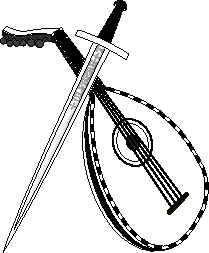
\includegraphics[width=0.33\textwidth]{sautoir-doud-et-dépée-monochrome.pdf}
  \captionsetup{labelformat=empty}
  \caption[Oud et épée ulfberht passés en sautoir]{}
  \index{Musique!Oud} \index{Guerre!Epee@Épée}
\end{figure}

  Ce film me démangeait de nouveau, tant j’avais de choses à demander à son réalisateur alors présent, si bien qu’une idée chassant l’autre, je ne pus toutes les poser. Finalement, j’ai pu demander à M.\,Lahcen \textsc{Zinoun} si la ressemblance entre certaines scènes et les odalisques d’\textsc{Ingres} n’étaient qu’un effet de ma sur-interprétation ou bien une référence voulue. Si je vous demandais de deviner ce qu’il me dit, c’est que dans ma question réside déjà la réponse; eh bien il me confirma son intention de faire allusion aux toiles d’\textsc{Ingres}.

  \paragraph{}
  Mais devinez d’abord qui m’accompagna ce jour là à la projection de ce film. Sauf que, là non plus, je ne peux vous poser cette énigme sans que vous ne vous doutassiez déjà de la réponse car évidement que j’étais avec Inès.
\end{prose}

\poemtitle{Premier milieu stratégique}\index{Guerre!Stratégie}\index{Femmes}
%\setIndexNameEntry[]{}
\begin{verse}%
  \quatrain%
  \metric{12}\metric{8}\metric{9}%
  Ter, mer, ciel, espace, et jusqu’au cyber-espace\\  % 
  Tels sont les cinq milieux que l’on enseigne aux classes\\  % 
  Mais le plus ancien de ceux que connaît la guerre\\  % 
  Dans les écoles d’armée ne s’enseigne guère.

  Car si la guerre est un récit\\  % 
  Qui s’écrit sur les corps aussi,\\  % 
  Ceux des femmes sont palimpsestes des amants\index{Ecriture@Écriture}\\  % 
  Mais meurtris des conflits, ils ne sont qu’ostracons.\index{Guerre!Traumatisme}

  Un champs certes sont les corps des femmes\\  % 
  Est-ce de bataille ou de labour ?\\  % 
  Rien n’est moins sûr dans cet amalgame\\  % 
  Où la guerre se mêle à l’amour.
\end{verse}


\poemtitle{Nakano Takeko}\index{Guerre!Généraux historiques}\index{Japon}\index{Guerre!Guérrières}\index{Epique@Épique}
%\setIndexNameEntry[]{}
\begin{verse}%
  \sizain%
  \metric{6}%
  \rhyme{e}%
  \rhyme[etain]{étain}%
  \rhyme[en]{[e\textbar{}o]n}%
  Nakano, tel le feu\index{Feu},\\  % 
  Sous cloche, elle s’éteint\\  % 
  Mais libre elle s’étend,\\  % 
  Dans un élan fougueux\\  % 
  Fait de cuivre et d’étain\\  % 
  Jusqu’à l’ignition.
\end{verse}

\poemtitle{Poliorcète}\index{Guerre!Poliorcétique}\index{Epique@Épique}
%\setIndexNameEntry[]{}
\begin{verse}%
  \quatrain%
  \metric{10}\metric{11}%
  \rhyme{en}%
  \rhyme[ete]{ète}%
  Par son regard\index{Femmes!Yeux} de braise\index{Feu} si ardent\\  % 
  Qui consuma mon cœur lors de la défaite,\\  % 
  Je prends d’assaut le sien en poliorcète,\\  % 
  Autant assiégé qu’assiégeant.\index{Amour}
\end{verse}

\poemtitle{Café turque}\index{Café}\index{Epique@Épique}
\setIndexNameEntry[Cafe turque]{Café turque}
\begin{verse}%
  \quatrain%
  \metric{8}\metric{10}%
  \rhyme{oir}%
  \rhyme{cho}%
  \rhyme{ay}%
  \rhyme{isc}%
  \rhyme{ay}%
  \rhyme{ieu}%
  \rhyme{or}%
  Constantinople\index{Histoire!Histoire arabo-musulmane} prise par l’ivoire,\\  % 
  Même mille fois, ne saurait valoir\\  % 
  Ô Turques, votre plus grande victoire,\\  % 
  Celle du café que je m’en vais boire.

  Contre les croisés, peu me chaud\\  % 
  L’issue de toutes vos batailles\\  % 
  Car avec le breuvage chaud\\  % 
  Il n’est de querelle qui vaille.

  Les épices, comme autant d’odalisques,\\  % 
  Valent toutes les femmes du sérail.\\  % 
  La brune au goût de musc à peine bisque\\  % 
  Ou la rousse\index{Femmes!Rousseur} de cannelle m’assaillent.

  Que d’autres Talas\index{Histoire!Histoire de Chine}\endnote{Bataille de la rivière Talas ayant opposé le califat abbasside à la dynastie Tang pour le contrôle de la Transoxiane et au cours de laquelle les mercenaires turques Karlouks alliés des Chinois font volte-face au profit des Abassides ancrant depuis lors les peuple turques dans le monde musulman.} aient encore lieu,\\  % 
  \incise{Cent Talas} pour qu’autant de fois encore\\  % 
  Soit notre ce café délicieux,\\  % 
  Et le papier\endnote{Il est probable que les captifs Chinois faits par les Abbassides au cours de la bataille de Talas aient introduit dans le monde musulman les techniques de fabrication du papier, donnant par conséquent le coup d’envoit à l’âge d’or arabomusulman.} où j’écris ces mots d’or.\index{Ecriture@Écriture}\index{Propos réflexif}
\end{verse}

\poemtitle{La cours des Lions}\index{Al\,Andalous!Alhambra}
\setIndexNameEntry[cours des Lions]{La cours des Lions}
\begin{verse}%
  \quatrain%
  \metric{9}%
  \rhyme{aine}%
  \rhyme[e]{é}%
  \rhyme{oze}%
  \rhyme{or}%
  On s’assit aux bords d’une fontaine\index{Eau}\\  % 
  Dont les flots, de nuit, nous arrosaient\\  % 
  Abreuvant nos paroles mondaines\\  % 
  Quand fût conviée la roseraie.\index{Fleur}

  Ayant palabré de tant de choses\\  % 
  Jusqu’aux primes lueurs de l’aurore\\  % 
  Où nous devinrent bouton de rose,\\  % 
  Je ne su si nous pouvions éclore.
\end{verse}

\poemtitle{L’Antisocrate}
\setIndexNameEntry[Antisocrate]{L’Antisocrate}
\begin{verse}%
  \quatrain%
  \metric{12}%
  \rhyme{u}%
  \rhyme[esse]{èsse}%
  Ses paroles, je les bu comme la ciguë\\  % 
  Mais ce fut moins pour avoir eu de la sagesse\\  % 
  Que pour en avoir alors été dépourvu,\\  % 
  Tant elles m’enivrèrent de leste allégresse.\index{Amour}
\end{verse}


\poemtitle{Signum minimum}\index{Epique@Épique}
%\setIndexNameEntry[]{}
\begin{verse}%
  \quatrain%
  \metric{10}\metric{11}%
  \rhyme{tane}%
  \rhyme{ove}%
  \rhyme{uc}%
  \rhyme{tan}%
  \rhyme[ele]{èle}%
  \rhyme[ze]{zé}%
  On dormit dans la nuit\index{Nuit} de Talassemtane\index{Femmes}\\  % 
  Entre les montagnes et les bêtes fauve\\  % 
  Avec la voûte céleste pour alcôve\\  % 
  Dont s’accommoda avec joie ma sultane.

  L’enlaçant de mes ailes de grand-duc,\\  % 
  Mon souffle chaud lui caressant la nuque,\\  % 
  Je lui susurrait à l’oreille en chuintant :\\  % 
  \enquote{Y a-t-il plus heureux que nous en cet instant ?}

  Mais qu’avait-elle besoin de répondre, elle,\\  % 
  Quand les fières étoiles peuplant le ciel\index{Astronomie}\\  % 
  Qui flottent solitaires aux alizés,\\  % 
  Lasses de nous admirer, nous jalousaient ?
\end{verse}


\begin{prose}
  Je suis tombé devant une copie du \work{Massacre des Abencérages}\index{Al\,Andalous!Abencérage} de Mariano \textsc{Fortuny}\index{Artistes!Mariano \textsc{Fortuny}} qui me saisit d’effroi, non pas tant pour le sujet sinistre et lugubre représenté, que par la violence par laquelle j’y fût projeté. Je m’actualisais immédiatement dans ce tableau où comme par réalité augmenté, je me suis retrouvé. J’aurais pu me mouvoir au sein de cette cours des Lions, sentir sur la plante de mes pieds le sang frais du gisant où j’ai marché, tant je me suis senti familier du propos.

  Aussi ai-je ressenti… ou plutôt ai-je été saisi par l’effroi du thème abordé, celui de la dramatique chute des Abencérages qui n’est qu’un prélude à celui du royaume de Grenade et enfin d’Al\,Andalous. Et spontanément, les vers s’imposèrent à moi en latin.
\end{prose}

\poemtitle{\xenism{Abenceragi} — Abencérages}\index{Epique@Épique}
\setIndexNameEntry[Abenceragi]{\xenism{Abenceragi} — Abencérages}
\setlength\LTleft{-1.7cm}%
\begin{verse}%
  \quatrain%
  \metric{12}%
  \rhyme{ni}%
  \rhyme{ate}%
  \rhyme{isse}%
  \rhyme{ite}%
  Abenceragi\endnotemark[\getrefnumber{foot.Abencerage}]\index{Al\,Andalous!Abencérage}, vos Elviræ domini,           \\  % 
  Sanguis\index{Guerre!Sang} vester Alhambræ\index{Al\,Andalous!Alhambra} fontem\index{Eau} adaquat,  \\  % 
  Quæ suum nomen numquam tam bene gerebat. \\  % 
  Non potentes estis sed adberitani.     

  \emph{Abencérages, vous maitres de Grenade,}\\  % 
  \emph{Votre sang abreuve les fontaines de l’Alhambra,\endnote{Allusion à la légende de leur éxtermination dans un bain de sang dont on raporte : \enquote{La fontaine d’apparat ne laissait plus couler de l’eau, mais leur sang…}.}}\\  % 
  \emph{Qui jamais ne portât aussi bien son nom.\endnote{\autonym{Alhambra} de l’arabe \textarabic{الحمراء}, voulant dire \autonym{La Rouge}.}}\\  % 
  \emph{Vous n’êtes pas puissants mais adbéritains\endnote{À comprendre dans le sens que la poésie latine lui donne de \emph{sôt}, \emph{stupide}.}.}

  Damno vestram nefas rixam cum Ziridis\index{Histoire!Histoire arabo-musulmane}   \\  % 
  Quam totum Gratæ regnum tecum perdidit.\index{Al\,Andalous!Reconquista} \\  % 
  Si pater vester sutor fortasse fuierit, \\  % 
  	Infra antecessorum soleam nunc estis.\index{Destin}

  \emph{Maudite soit votre querelle avec les Zirides\endnote{Faction rivale des Abencérages dont le conflit ensanglanta Grenade au point d’en hâter la chute.}}\\  % 
  \emph{Où vous entrainâtes la destruction le royaume de Grenade}\\  % 
  \emph{Si votre père fut sans doute cordonnier\endnote{\autonym{Abencérage} de l’arabe \textarabic{بنو سراج}, voulant dire \enquote{fils de cordonier}.},}\\  % 
  \emph{Vous êtes sous les sandales de vos ancêtres désormais.}
\end{verse}

%\begin{longtable}{L{7.3cm} L{6.5cm}}
%\noalign{\poemtitle{Abencérages — \xenism{Abenceragi}}}
%\endfirsthead
%
%Abenceragi, vos Elviræ domini, & \emph{Abencérages\endnote{Famille puissante d’Al\,Andalous.}, vous maitres de Grenade,}\\  % 
%Sanguis vester Alhambræ fontem adaquat, & \emph{Votre sang abreuve les fontaines de l’Alhambra,\endnote{Allusion à la légende de leur éxtermination dans un bain de sang dont on raporte : \enquote{La fontaine d’apparat ne laissait plus couler de l’eau, mais leur sang…}.}}\\  % 
%Quæ suum nomen numquam tam bene gerebat. & \emph{Qui jamais ne portât aussi bien son nom.\endnote{\autonym{Alhambra} de l’arabe \textarabic{الحمراء}, voulant dire \autonym{La Rouge}.}}\\  % 
%Non potentes estis sed adberitani. & \emph{Vous n’êtes pas puissants mais adbéritains\endnote{À comprendre dans le sens que la poésie latine lui donne de \emph{sôt}, \emph{stupide}.}.}\\  % 
%\\  % 
%Damno vestram nefas rixam cum Ziridis & \emph{Maudite soit votre querelle avec les Zirides\endnote{Faction rivale des Abencérages dont le conflit ensanglanta Grenade au point d’en hâter la chute.}}\\  % 
%Quam totum Gratæ regnum tecum perdidit. & \emph{Où vous entrainâtes dans la destruction le royaume de Grenade}\\  % 
%Si pater vester sutor fortasse fuierit, & \emph{Si votre père fut peut-être cordonnier\endnote{\autonym{Abencerage} de l’arabe \textarabic{بنو سراج}, voulant dire \enquote{fils de cordonier}.},}\\  % 
%Infra antecessorum soleam nunc estis. & \emph{Vous êtes sous les sandales de vos ancêtres désormais.}
%\end{longtable}
%%\end{adjustwidth}

\poemtitle{Aube}
%\setIndexNameEntry[]{}
\begin{verse}%
  \quatrain%
  \metric{12}%
  \rhyme{sso}%
  \rhyme[fame]{fa[n\textbar{}m]e}%
  Les rayons du soleil\index{Astronomie!Soleil} comme autant de pinceaux\\  % 
  Peignent  la nuit\index{Nuit} lorsque s’en appose le sceau\\  % 
  En y parsemant la couleur chaire des femmes\index{Femmes}\\  % 
  Mais qui, à l’arrivée de l’aurore, se fane.
\end{verse}

\poemtitle{Exhortation au troubadour}\index{Musique}
%\setIndexNameEntry[]{}
\begin{verse}%
  \distique%
  \metric{10}
  \rhyme[an]{[a\textbar{}e]n}%
  Ô troubadour, par des airs attrayants,\\  % 
  Captives-nous et déploie ton talent.
\end{verse}

\poemtitle{La Nébuleuse}\index{Astronomie}\index{Femmes}
\setIndexNameEntry[Nebuleuse]{La Nébuleuse}
\begin{verse}%
  \quatrain%
  \metric{11}%
  \rhyme[iel]{ièl}%
  \rhyme{leste}%
  Elle qui fut mon horizon et mon ciel,\\  % 
  Lorsqu’elle rougit à mes propos de miel,\\  % 
  C’est d’un crépuscule écarlate céleste\\  % 
  Dont se part son visage et ses gestes lestes.
\end{verse}

\poemtitle{Les enfants du soleil}\index{Astronomie!Soleil}\index{Epique@Épique}
\setIndexNameEntry[enfants du soleil]{Les enfants du soleil}
\begin{verse}%
  \quatrain%
  \metric{9}%
  \rhyme[eye]{èye}%
  \rhyme{aye}%
  Nous sommes les enfants du soleil.\\  % 
  À nous l’amour à chaque réveil\index{Amour}\\  % 
  Car, égaux, nous sommes tous pareils,\\  % 
  Chacun de nous est une merveille.

  Et s’allume dans nos yeux vermeil\\  % 
  La passion qui se délaye\\  % 
  Quand par les rayons l’on se fraye\\  % 
  Tous les chemins exceptionnels.
\end{verse}

\poemtitle{Le silence était d’elle}\index{Femmes}
%\setIndexNameEntry[]{}
\begin{verse}%
  \quatrain%
  \metric{12}%
  \rhyme[ere]{ère}%
  \rhyme[e]{é}%
  Elle se tait. Dois-je m’exprimer ou me taire ?\\  % 
  Commenter la perfection la gâterait,\\  % 
  Mais, dans le cas contraire, ne guère parler\\  % 
  Laisserait croire qu’elle puisse me déplaire.
\end{verse}

\begin{prose} 
  Ne pouvant me résoudre à ne guère aborder de nouveau le cycle \work{Dune}, il me fallut, presque par la force de la nécessité en écrire encore quelques vers, comme autant de précieuses lampées d’eau que l’on craint de verser sur le sable. Et alors que l’excellentissime M.\,Hans \textsc{Zimmer}\index{Artistes!Hans \textsc{Zimmer}}\index{Cinéma}\index{Musique} fut à l’œuvre dans la musique de l’adaptation cinématographique qui en fût faite récemment, c’est en vérité son travail sur le non moins mémorable \work{Interstellaire} qui accompagna \incise{non, que dis-je ?} qui \autonym{enjoignît} mon écriture.
\end{prose}

\poemtitle{Amour sur Arrakis\endnotemark[\getrefnumber{foot.DuneArrakis}]}\index{Dune}
\setIndexNameEntry{Amour sur Arrakis}
%\renewcommand\currentpoemtitle{Amour sur Arraki}%
\index{Epique@Épique}
\begin{verse}%
  \sizain%
  \metric{8}\metric{10}%
  \rhyme{o}%
  \rhyme{charné}%
  \rhyme{olisse}%
  %
  \rhyme{e}%
  \rhyme{eur}%
  \rhyme{iade}%
  %
  \rhyme{oi}%
  \rhyme{eur}%
  \rhyme[en]{[e\textbar{}o]n}%
  %
  \rhyme[ene]{ène}%
  \rhyme[ere]{ère}%
  \rhyme{oi}%
  %
  \rhyme{ile}%
  \rhyme{itre}%
  \rhyme{ife}%
  Dans l’ivresse de l’orgie tau\endnote{Dans l’œuvre de Frank \textsc{Herbert} il s’agit d’orgies sacrées et ritualisées du peuple Fremen.},\\  % 
  Je l’ai aimée à en perdre la peau,\\  % 
  Jusqu’à en être décharné\\  % 
  Comme emporté par la Coriolis\endnote{Type de tempête mortelle dans l’univers de \work{Dune}.},\\  % 
  Autant étreint par sa peau lisse,\\  % 
  Qu’enlacé de ses deux bras acharnés.

  Me mirant dans son regard bleu\index{Femmes!Yeux},\\  % 
  Le regard de l’ibad\endnotemark[\getrefnumber{foot.regardibad}], serti d’ardeur\\  % 
  Me dit combien elle me veut,\\  % 
  Qu’elle me désir à pleine fureur\\  % 
  En combattante du jihad\\  % 
  Qui lutte sur Dune pour notre dyade.

  Ô sayyadina\endnote{Sorte de prétresse des Fremen qui guide l’orgie tau.}, hâte-toi\\  % 
  Et transmute l’eau-de-vie du faiseur\endnote{Le faiseur est une créature sécrétant une eau toxique tant que la sayyadina n’y pratique pas un rituel qui la rend potable.}\\  % 
  Afin que le sietch\endnote{Sorte de communauté villageoise de Fremen vivant dans le désert.} en boit\\  % 
  Afin que la fremen m’aime sur l’heure\\  % 
  Et que dans les couloirs du temps,\\  % 
  Avec euphorie nous y entrions.

  Ma belle et puissante Fremen,\\  % 
  L’âme affûtée par le vent du desert,\\  % 
  À la peau de sable et d’ébène,\\  % 
  Que l’existence parait si légère\\  % 
  Lorsque je demeure sans voix\endnote{Double sens avec la \autonym{Voix} qui est une capacité qu’acquièrent certaines personnes exceptionnelles dans l’univers de fiction de \work{Dune}.},\\  % 
  Lorsque ton regard se pose sur moi.

  Dégrafant si tôt le distyle\endnote{Vêtement des Fremen qui leur permet de survivre aux rigueurs du désert.}\\  % 
  	Et négligeant sur le sol la jolitre\endnote{Gourde utilisée par les Fremen pour garder l’eau dans le désert.}\index{Eau}\\  % 
  Pour se donner au jeu subtile\\  % 
  Que l’on reportera sur tant d’épîtres\\  % 
  En or et en hiéroglyphes\index{Ecriture@Écriture!Hiéroglyphes}\\  % 
  Et dont se souviendront les apocryphes.

  Tressaille, fille d’Arrakis.\\  % 
  Oh oui, tressaille de cette allégresse\\  % 
  Dont t’aura enivrée l’épice.\\  % 
  Que soit portés haut tes cris de liesse,\\  % 
  Qu’ils s’oient bien au delà de Dune\\  % 
  Et s’entendent plus loin que ses deux lunes.\endnote{Autour de la planète Arrakis orbitent effectivement deux lunes.}
  %
  \rhyme{isse}%
  \rhyme[esse]{èsse}%
  \rhyme{une}%
\end{verse}

\poemtitle{Halène}\index{Femmes}
%\setIndexNameEntry[]{}
\begin{verse}%
  \quatrain%
  \metric{11}%
  \rhyme[esse]{èsse}%
  \rhyme[ertisse]{értisse}%
  Et son halène chaude qui me caresse\\  % 
  Me fait déjà une secrète promesse,\\  % 
  Avant que ses lèvres tendres me sertissent\\  % 
  Invitant à un langoureux interstice.
\end{verse}

\poemtitle{Rien de plus}\index{Femmes}
%\setIndexNameEntry[]{}
\begin{verse}%
  \distique%
  \metric{12}%
  \rhyme[ere]{ère}%
  Et tout ce que contiennent le ciel et la terre\\  % 
  Ne saurait autant que le soleil\index{Astronomie!Soleil} te parfaire.
\end{verse}

\poemtitle{Danse de feu}\index{Feu}
%\setIndexNameEntry[]{}
\begin{verse}%
  \quatrain%
  \metric{12}\metric{11}%
  \rhyme{vera}%
  \rhyme{eur}%
  De la lave qu’à travers mes yeux\index{Femmes!Yeux} l’on versa,\\  % 
  Que cette danse qui consume mon cœur\\  % 
  D’un corps liquide qui fait suinter ma sueur.\\  % 
  En un instant, elle nous bouleversa.
\end{verse}

\poemtitle{Ordre de bataille}\index{Guerre!Bataille}\index{Epique@Épique}
%\setIndexNameEntry[]{}
\begin{verse}%
  \quatrain%
  \metric{10}%
  \rhyme{onde}%
  \rhyme[piere]{pière}%
  Les arcs, les arbalètes, et les frondes\\  % 
  Font pleuvoir une nuée qui abonde\\  % 
  De flèches, de vifs carreaux, et de pierres\\  % 
  Qui choient autant que tombent les paupières.
\end{verse}


\section*{Didaxie}
\markboth{}{Didaxie}
\addcontentsline{toc}{section}{Didaxie}

\poemtitle{La vie, ses peines, et ses dilemmes}\index{Humour}
\setIndexNameEntry[vie, ses peines, et ses dilemmes]{La vie, ses peines, et ses dilemmes}
\begin{verse}%
  \quatrain\distique%
  \metric{9}\metric{10}%
  \rhyme[eme]{ème}%
  \rhyme[ese]{èze}%
  \rhyme{a}%
  \enquote{Face à la vie et à ses dilemmes,\\  % 
  Il n’existe rien de plus à même\\  % 
  De panser chacun des maux qui lèsent\\  % 
  Que le \work{concerto d’Aranjuez.}\index{Musique}}

  Nous dit le poète. Mais alors moi,\index{Propos réflexif}\\  % 
  Je crois que c’est plutôt le chocolat !
\end{verse}

\begin{prose}
D’amblais, il me sembla voir une proximité phonétique entre les mots latin d’\autonym{enfant}, \autonym{livre}, et \autonym{liberté}. Serait-ce sans doute parce que les livres libèrent les enfants ? Ce qui se dit :
\end{prose}

\addcontentsline{toc}{subsection}{Maxime de la libération par les livres}
\subparagraph{}
Libri libros liberant.

\poemtitle{Du tennis de table}
\setIndexNameEntry[tennis de table]{Du tennis de table}
\begin{verse}%
  \haiku
  J’entends ping et pong,\\  % 
  Et je tape, paf, la balle\\  % 
  Qui bondi et tombe.
\end{verse}

\begin{figure}[h]
  \centering
  
\includegraphics[height=1cm]{balancoire.pdf}
  \captionsetup{labelformat=empty}
  \caption[Idéotexte de \autonym{balançoire}]{}
\end{figure}

\begin{prose}
  Il y avait, je ne me souviens plus quand exactement, un enfant à qui je devais, pour lui donner un cours de langue, lui illustrer que notre langue n’est pas à la vérité des plus aisées. Je lui donnais l’exemple des mots du cheval et la grande variété des racines pour les former.
\end{prose}


\poemtitle{Les mots du cheval}\index{Chevaux}
\setIndexNameEntry[mots du cheval]{Les mots du cheval}
\begin{verse}%
  \distique%
  \metric{5}\metric{6}\metric{7}
  \rhyme{al}%
  \rhyme[an]{[a\textbar{}e]n}%
  \rhyme{lin}%
  \rhyme{gre}%
  \rhyme[en]{[e\textbar{}o]n}%
  \rhyme[e]{é}%
  \rhyme{froi}%
  \rhyme[lie]{lié}%
  \rhyme[e]{é}%
  \rhyme{pic}%
  \rhyme[en]{[e\textbar{}o]n}%
  \rhyme{an}%
  Prenons un animal,\\  % 
  Au hasard, le \autonym{cheval}.

  Sa femelle, la \autonym{jument}\\  % 
  Est une douce maman.

  Elle fait des câlins\\  % 
  À son petit \autonym{poulain}.

  Si jamais on le fait \autonym{hongre},\\  % 
  il deviendra castré, bigre !

  S’il en est autrement,\\  % 
  Il sera \autonym{étalon}.

  Luttant avec fierté,\\  % 
  Il sera le \autonym{destrier}

  Ou distant de l’effroi\\  % 
  En charmant \autonym{palefroi}.

  Scellé par un \autonym{écuyer},\\  % 
  Il mène le \autonym{cavalier}.

  Ou au jeu de la paix,\\  % 
  Par le beau \autonym{jokey}

  Dans une course \autonym{hippique}\\  % 
  Qui sera aussi épique

  Que nous croyons souvent\\  % 
  Être \autonym{équitation}.

  Ferre-toi auparavant\\  % 
  Par le \autonym{maréchal-ferrant}.
\end{verse}



\section*{Courtes épopées d’arc et de dague}
\markboth{}{Courtes épopées d’arc et de dague}
\addcontentsline{toc}{section}{Courtes épopées d’arc et de dague}
\poemtitle{Exorde à l’archer}\index{Epique@Épique}
%\setIndexNameEntry[]{}
\begin{verse}%
  \quatrain%
  \metric{10}\metric{13}\metric{12}\metric{11}
  \rhyme{oche}%
  \rhyme[ere]{ère}%
  \rhyme[ene]{ène}%
  \rhyme[e]{é}%
  \rhyme{e}%
  Tapisse-toi derrière le merlon et encoche\index{Archerie}\\  % 
  La flèche perçant le catafractaire\index{Guerre!Chevalerie} en approche.\\  % 
  Tiens-toi devant le créneau et libère\\  % 
  La flèche traçant la cuirasse fière.

  Dégaine l’épée\index{Guerre!Epee@Épée} à la lame damascène,\\  % 
  Suspend-en promptement de l’assaillant l’allène.\\  % 
  Et le sang\index{Guerre!Sang} qui ruissellera sur le moiré,\\  % 
  Séché, sera donc legs à la postérité.

  Les faisceaux indéfectibles, par la guivre,\\  % 
  Seront noués de sa dépouille languide.\\  % 
  Exorde aux justes de s’y rallier\\  % 
  Et rappel de l’engeance terrassée.
\end{verse}

\poemtitle{Les dagues des meurtrières}\index{Epique@Épique}
\setIndexNameEntry[dagues des meurtrières]{Les dagues des meurtrières}
\begin{verse}%
  \quatrain%
  \metric{10}\metric{14}%
  \rhyme[en]{[e\textbar{}o]n}%
  \rhyme[ere]{ère}%
  Les cheveux bouclés\index{Femmes!Cheveux} qui flottent au vent\\  % 
  Sont la bannière de celles aux charmes ondulants.\\  % 
  Coiffées d’autant de dagues meurtrières,\\  % 
  Livrant l’ennemi aux sinuosités de la guerre.\index{Guerre!Guérrières}
\end{verse}

\poemtitle{Le sang ennemi}\index{Guerre}\index{Guerre!Sang}\index{Epique@Épique}
\setIndexNameEntry[sang ennemi]{Le sang ennemi}
\begin{verse}%
  \quatrain%
  \metric{12}%
  \rhyme{verse}%
  \rhyme{i}%
  Que toujours dans nos coupes, vermeils se déversent\\  % 
  Les torrents qui affluent des régiments occis.\\  % 
  Que toujours dans nos coupes, le sang ennemi\\  % 
  Pleuve jusqu’au buvant et remplisse en averses.
\end{verse}



\section*{Constellation du Loup}
\markboth{}{Constellation du Loup}
\addcontentsline{toc}{section}{Constellation du Loup}\index{Femmes}
\poemtitle{α Lupi}
\setIndexNameEntry[a Lupi]{α Lupi}
\begin{verse}%
  \quatrain%
  \metric{11}%
  \rhyme{passe}%
  \rhyme{or}%
  %
  \rhyme{i}%
  \rhyme{o}%
  %
  \rhyme{ante}%
  \rhyme[eze]{èze}%
  %
  \rhyme[an]{[a\textbar{}o]n}%
  \rhyme[e]{é}%
  %
  \rhyme{ope}%
  \rhyme{iene}%
  %
  \rhyme{rian}%
  \rhyme{loi}%
  %
  Tant de choses renferme le vaste espace\index{Astronomie}\\  % 
  Mais hélas bien peu me chaud ce qui s’y passe.\\  % 
  D’entre Balance, Scorpion, ou Centaure,\endnote{La constellation du Loup se trouve entre celles des Balance, Scorpion, et Centaure.}\\  % 
  Seule la plus brillante étoile j’explore.

  Les longs cheveux\index{Femmes!Cheveux} noirs de la Beta Cephei\endnote{Les étoiles variables de type Beta Cephei, ou par métonymie les Beta Cephei constituent une catégorie d’étoiles dont fait parti l’alpha Lupi.}\\  % 
  Sont des cordes de violon attendries.\\  % 
  Délaissant l’archer pour un pizzicato\index{Musique}\endnote{Technique de violon consistant à pincer les cordes des doigts au lieu d’utiliser l’archer.},\\  % 
  S’y glissent les doigts qui jouent l’adagio\endnote{Deuxième mouvement du \work{Concerto d’Aranjuez} composé par Joaquín \textsc{Rodrigo}.}.

  S’effilent de ses rayons des notes si charmantes\\  % 
  Que l’on veut toujours longues et éclatantes.\\  % 
  Qu’elles ne s’éteignent pas ces quelques braises,\\  % 
  Ces notes du \xenism{Concerto de Aranjuez}.

  Les savourant de grande admiration,\\  % 
  Je perçois de l’or et tant de diamants\\  % 
  Dans la voix qui perce le cosmos entier.\\  % 
  Il n’est désormais plus Férmi\endnote{Jeu de mot avec le paradoxe de Fermi. Du nom du prix Nobel de physique qui postula une série d’observations et émis des hypothèses au sujet de l’existence de civilisations extraterrestres.} d’en douter.

  Perclus de doutes devant le télescope,\\  % 
  Au souvenir de la cartomancienne\\  % 
  Qui d’Ézéchiel\endnote{Allusion à la carte du Monde dans le tarot de Marseille laquelle arbore le thème du tétramorphe tel que décrits dans la vision d’Ézéchiel.} tira une antienne,\\  % 
  Je vis mes tripes dans les vases canope.\index{Egypte@Égypte}

  Mugissant, glatissant, rugissant, priant\endnote{Chaque cris représente l’un des \enquote{quatre vivants}. Le taureau pour le mugissement, l’aigle pour le glatissement, le lion pour le rugissement, et l’ange pour la prière.}\\  % 
  L’arcane émeut l’âme en se l’appropriant.\\  % 
  Le Monde qui mit le monde sous des lois,\\  % 
  Que gueux et rois admirent de bon aloi.
\end{verse}

\poemtitle{Les feux de tes yeux}\index{Feu}\index{Femmes!Yeux}\index{Epique@Épique}
\setIndexNameEntry[feux de tes yeux]{Les feux de tes yeux}
\begin{verse}%
  \distique%
  \metric{10}\metric{9}\metric{8}\metric{7}\metric{6}\metric{5}\metric{4}\metric{3}\metric{2}\metric{1}
  \rhyme{eu}%
  \rhyme{a}%
  \rhyme{a}%
  \rhyme{tion}%
  \rhyme[ele]{èle}%
  \rhyme{iye}%
  \rhyme{fer}%
  \rhyme{eu}%
  \rhyme{eu}%
  Dans l’ardeur calcifère de tes yeux,\\  % 
  Se déchaîne ici-bas un ardent feu.

  Incendie dont tout l’apostolat\\  % 
  Étend loin ses flammes et ses bras.

  Au delà de l’Himalaya\\  % 
  Et encore bien au delà,

  Déclenche l’ignition\\  % 
  Qui est la séduction.

  Pares-moi de tes ailes,\\  % 
  Que j’atteigne le ciel.

  Comme ta pupille,\\  % 
  La terre scintille

  Dans l’atmosphère\\  % 
  Où  prolifèrent

  Tous les feux\\  % 
  De tes yeux.

  Les feux\\  % 
  Des yeux,

  De\\  % 
  Tes\\  % 
  Yeux.
\end{verse}




\begin{prose}
  C’est en sa compagnie à elle, Alpha du Loup, que s’affermit mon goût pour la synthwave qui s’était auparavant manifesté. Que n’ai-je appris d’elle, au risque de paraphraser les poèmes où j’en parles déjà.
  Et je devrais, pour rendre grâce à l’influence \incise{au rayonnement, allais-je dire} qu’elle eu sur moi en dire beaucoup plus que ces quelques poèmes, mais je trouvais qu’il y avait, là concernant, grande élégance dans la brièveté.
\end{prose}

\begin{prose}
  Du reste, combien même sais-je l’image de la \enquote{bande sonore d’une existence} éculée, qu’elle constitue un lieu commun que je suis le premier à abhorrer, il n’empêche que le morceau \work{Plastic love} et d’autres encore, plus que jamais m’évoquent la période où je rencontrai l’étoile du Loup.
\end{prose}

\poemtitle{Maria \textsc{Takeuchi}}\index{Synthwave}\index{Japon}
%\setIndexNameEntry[]{}
\begin{verse}%
  \haiku%
  \rhyme{ve}%
  Dans mon rêve mauve\\  % 
  Elle, Maria {Takeuchi}\endnote{Allusion à la chanteuse de city pop Maria \textsc{Takeuchi} et à sa chanson プラスチック・ラブ sortie en 1984 connue sous le nom international de \work{Plastic love}, et plus exactement à la résurgence de l’intérêt dont elle fit preuve en 2017 à la faveur d’un algorithme de recommandation et de la popularité des genres esthétiques vaporwave et synthwave qui accompagnent cette période. Autrement dit, cette chanson n’aura connu de succès que trente-trois ans après sa publication. Le regain de popularité pour ce morceau ayant donné lieu à de nombreuses reprises, il me semble qu’est fait ici allusion aussi bien à l’œuvre originale qu’à ses dérivées,  notamment \work{Plastic Love (cyberpunk/synthwave remix)} par Astrophysics publiée en 2020 mars 31.},\\  % 
  Chantait en synthwave.
\end{verse}

\begin{figure}[h]
  \centering
  
\includegraphics[height=1cm]{piano.pdf}
  \captionsetup{labelformat=empty}
  \caption[Idéotexte de \autonym{balançoire}]{}
\end{figure}

\begin{prose}
  Je ne devrais plus rien ajouter d’autre la concernant, à elle qui composa pour moi de jolies chansons sur son piano, et qui aurait encore probablement fait des symphonies si je n’avais pas fais le con. Mais autant qu’un ivrogne qui prendrait un dernier verre pour la route, je prendrais moi aussi un dernier vers.
\end{prose}

\poemtitle{Affliction}\index{Propos réflexif}
%\setIndexNameEntry[]{}
\begin{verse}%
  \quatrain%
  \metric{12}%
  \rhyme{oir}%
  \rhyme{ume}%
  Aussi tuméfié que moi par le miroir,\\  % 
  Ô Quetzalcóatl\index{Mythologie}, laisse tomber quelques plumes\\  % 
  %De grâce, laisse en plusieurs encore choir\\  % 
  %Qu’il y en ai assez pour le mal qui m’allume,\\  % 
  Que je m’en saisisse et écrive mes déboires,\\  % 
  Que je puisse en transcrire toute l’amertume.
\end{verse}

\section*{Vers d’autres horizons}%
\markboth{}{Vers d’autres horizons}%
\addcontentsline{toc}{section}{Vers d’autres horizons}%

\poemtitle{Laurier éclatant}
%\setIndexNameEntry[]{}
\begin{verse}%
  \quatrain%
  \metric{12}%
  \rhyme{tion}%
  \rhyme{itre}%
  Le laurier\index{Fleur} qui explose en mille émotions,\\  % 
  Lance ses fleurs dans toutes les directions,\\  % 
  Sous lesquelles les rayons du soleil\index{Astronomie!Soleil} s’infiltrent,\\  % 
  Et de l’astre lumineux apportent l’épître.
\end{verse}

\begin{floatpoem}
  \poemtitle{Pyramide de Khéops}\index{Egypte@Égypte}\index{Epique@Épique}%
  \calligramme%
  \begin{center}
    \setstackTAB{&}%
    \fixTABwidth{T}%
    \sbox1{\marginnote{\endnote{\autonym{Kêmi} ou \autonym{Kemet} est le nom qu’attribuaient les Égyptiens antiques à leur pays. Il se traduirait d’après les égyptologues par \enquote{Terre noire}.}}}
    \sbox2{\marginnote{\endnote{Snéfrou est père de Khéops.}}}
    \sbox3{\marginnote{\endnote{Djédefrê est fils de Khéops.}}}
    \sbox4{\marginnote{\endnote{Anubis est le dieu de la mythologie égyptienne vers lequel se rendent les âmes des défunts après leur inhumation, et notamment vers lequel se rendent les âmes des pharaons après que leur tombeau ai été scellé dans la pyramide.}}}
    \tabbedCenterstack{
      ~&~&~&~&~&~&~&~&~&~&~&Ô&~&~&~&~&~&~&~&~&~&~&~\\  % 
      ~&~&~&~&~&~&~&~&~&~&P&I&C&~&~&~&~&~&~&~&~&~&~\\  % 
      ~&~&~&~&~&~&~&~&~&S&A&C&R&É&~&~&~&~&~&~&~&~&~\\  % 
      ~&~&~&~&~&~&~&~&D&E&·&K&Ê&M&I\rlap{,}\rlap{\,\copy1}&~&~&~&~&~&~&~&~\\  % 
      ~&~&~&~&~&~&~&B&E&A&U&T&É&·&E&T&~&~&~&~&~&~&~\\  % 
      ~&~&~&~&~&~&S&U&P&É&R&I&O&R&I&T&É&~&~&~&~&~&~\\  % 
      ~&~&~&~&~&T&O&N&·&I&M&M&E&N&S&I&T&É&~&~&~&~&~\\  % 
      ~&~&~&~&F&A&I&T&·&À&·&L&’&É&G&Y&P&T&E\rlap{.}&~&~&~&~\\  % 
      ~&~&~&T&U&·&F&U&S&·&A&U&·&P&R&E&M&I&E&R&~&~&~\\  % 
      ~&~&D&E&·&S&N&É&F&R&O&U\rlap{\,\raisebox{0.5ex}{\copy2}}&·&E&T&·&A&Ï&E&U&L&~&~\\  % 
      ~&D&E&·&D&J&É&D&E&F&R&Ê\rlap{\,\copy3}&,&·&L&A&·&R&A&M&P&E&~\\  % 
      V&E&R&S&·&L&E&S&·&V&O&I&E&S&·&D&’&A&N&U&B&I&S\rlap{.}\rlap{\,\copy4}
    }
  \end{center}
\end{floatpoem}

\begin{prose}
  Je tâchais dans ce recueil de poèmes tout au long de sa composition de demeurer simple. Après tout, Sun Tzu ne dit-il pas si bien :

  \begin{quotation}
    Il arrive qu’étant parvenu à se hisser jusqu’au bon, l’on puisse aller encore au delà. Mais ce qui est au dessus du bon n’est point le bon lui même.
  \end{quotation}

  Je ne sais si j’y suis parvenu mais au moins, je m’y serais efforcé.
\end{prose}

\begin{prose}
  Que dire encore, sinon que je me souviens que lorsque F***** m’emmena sur les remparts de la cité portugaise d’Eljadida, elle m’entraina jusqu’à un mirador où notre intimité ne fût rompue que par un rayon de lumière.
\end{prose}

\poemtitle{Ruban de lumière}
%\setIndexNameEntry[]{}
\begin{verse}%
  \quatrain%
  \metric{11}%
  \rhyme[iere]{ière}%
  \rhyme{eu}%
  Un éphémère ruban fait de lumière\\  % 
  Se faufila à travers la meurtrière\index{Archerie}\\  % 
  Et alla se nouer autour des cheveux\index{Femmes!Cheveux}\\  % 
  Au complexe réseau de mèches en feux.\index{Feu}
\end{verse}

\poemtitle{Mont Fuji}\index{Japon}\index{Propos réflexif}
%\setIndexNameEntry[]{}
\begin{verse}%
  \haiku%
  \rhyme{i}%
  Que dire, Fuji,\\  % 
  Qui ne l’eut déjà été\\  % 
  Quand ton nom suffit ?
\end{verse}

\poemtitle{Matins éternels}
%\setIndexNameEntry[]{}
\begin{verse}%
  \quatrain%
  \metric{12}%
  \rhyme{ivre}%
  \rhyme[nesse]{nèsse}%
  Si ce matin fut ravissant à m’en rendre ivre,\\  % 
  De tels, il y en eut tant avant que je naisse,\\  % 
  Il y en aura quand j’aurais cessé de vivre.\\  % 
  Mais de leurs éclats je n’aurais vu que vanesse.
\end{verse}

\poemtitle{En route vers le Falāĥ !}
%\setIndexNameEntry[]{}
\renewcommand\currentpoemtitle{En route vers le Falāĥ}%
\index{Epique@Épique}
\begin{verse}%
  \sizain%
  \metric{8}%
  \rhyme{one}%
  \rhyme{ar}%
  \rhyme[iere]{ière}%
  Sur le parvis de Babylone\\  % 
  Je franchis la porte d’Ishtar\\  % 
  En compagnie de mes lionnes.\\  % 
  Pouvais-je croire que derrière\\  % 
  Me parerais un éclat fière\\  % 
  Puisque là m’attendrait la gloire ?
\end{verse}

\poemtitle{La rencontre}\index{Café!Etablissement cafe@Établissement café}\index{Propos réflexif}
\setIndexNameEntry[rencontre]{La rencontre}
\begin{verse}%
  \distique%
  \metric{8}%
  \rhyme{pardevère}%
  Ça a commencé par deux verres\\  % 
  Et ça a fini par deux vers.
\end{verse}

\poemtitle{La paix}\index{Egypte@Égypte}
\setIndexNameEntry[paix]{La paix}
\begin{verse}%
  \quatrain%
  \metric{12}\metric{10}\metric{11}\metric{14}%
  \rhyme[e]{é}
  \rhyme{ic}
  %
  \rhyme{iye}
  %
  \rhyme{ambe}
  %
  \rhyme{osse}
  \rhyme[ezan]{éz[a\textbar{}e]n}
  %
  \rhyme{il}
  \rhyme{able}
  %
  \begin{minipage}{\linewidth}
    \raisebox{-\height+0.7cm}[0cm][0pt]{\hspace{-1.1cm}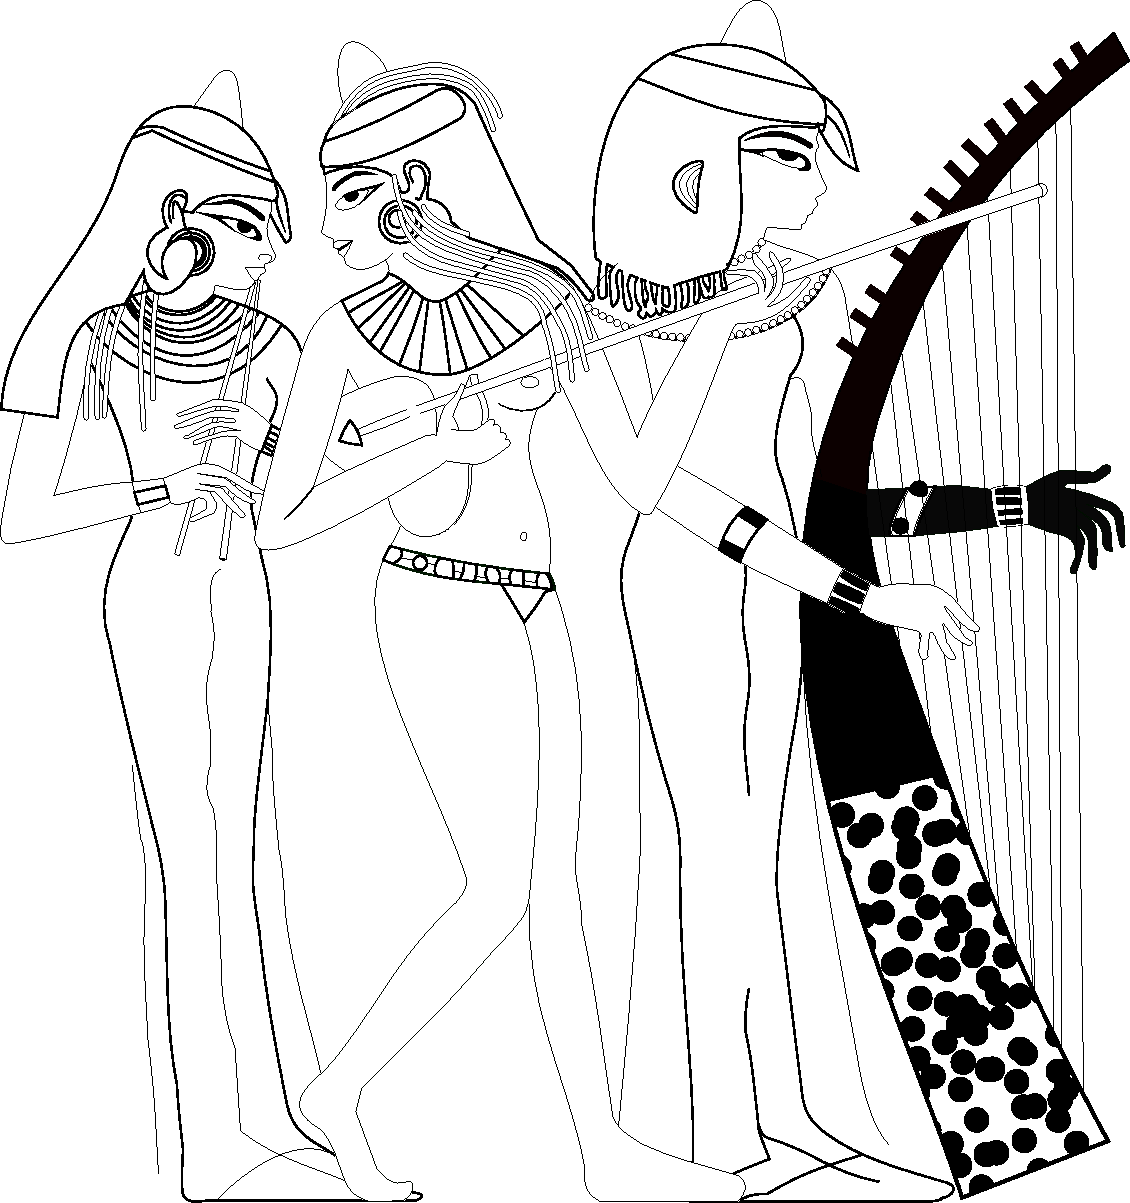
\includegraphics[width=1.5cm]{lettrine-E-trio-degyptiennes.pdf}}\addcontentsline{lof}{figure}{Lettrine \autonym{E} au trio de musiciennes d’après une fresque retrouvée dans la tombe de Nakht à Thèbes}%
    \textsc{coutez !}  La harpe d’Hathor\endnote{Déesse égyptienne de la musique, de l’amour, et de la joie.} est libérée.\index{Musique}\endnote{Prononcé par le personnage de la princesse Téti dans le dessin animé qui marqua mon enfance \work{Papyrus} au 16\ieme{} épisode.}\\\nopagebreak[4]
    \hspace{0.6cm}Et le cliquetis de la lance métallique\index{Guerre!Bellisonus}\\\nopagebreak[4]
    \hspace{0.6cm}N’est plus que musique lorsqu’à terre tombé.
  \end{minipage}\\\vspace*{0.4ex}
  Tandis que s’étreignent les corps diplomatiques.\index{Guerre!Paix}

  Archer, noue ta corde à cette cheville\index{Archerie},\\  % 
  Avec l’oud\index{Musique!Oud} rejoins l’orchestre sacré\\  % 
  Qui commémore la guerre achevée\\  % 
  Quand d’allégresse tressaillent les filles.

  Défaisant les sangles corsetant le pied,\\  % 
  De ses sandales elle s’est délestée\\  % 
  Et dans la marrée\index{Eau} elle mouille la jambe\\  % 
  Par un mouvement frêle, souple et ingambe.

  Monte plus haut réverbe de l’aulos\endnote{Instrument de musique à vent d’Égypte antique.}\\  % 
  Dont la Divinité est le présent,\\  % 
  Nous éloignant à jamais de l’atroce\\  % 
  Par ses parfums exquis et apaisants.

  Que les paupières se ferment entrainées par les cils\index{Femmes!Yeux}\\  % 
  Alourdis des gouttelettes qui abreuvent le Nil\index{Egypte@Égypte!Nil}\\  % 
  De ses généreux torrents d’eau fraîche et intarissable\\  % 
  Semblant chaudes lorsqu’elles aspergent nos corps aimables.
\end{verse}


\newpage
\thispagestyle{empty}
\null\cleardoublepage
\section*{Épilogue}
\thispagestyle{empty}
\markboth{}{Épilogue}%
\addcontentsline{toc}{section}{Épilogue}%
%\chapter{Divers}
%
{\em\small
  Vous savez, à l’issue de la compilation de ce recueil, les bêta-lecteurs s’exclamèrent dès lors qu’ils en eurent connaissance \enquote{Mais ça a dû te \emph{prendre} du temps !}, ce qui me sidéra à chaque reprise.

  Dans la mesure où tout au contraire, écrire ces vers me \emph{donna} du temps. Chaque lettre de ces poèmes est un grain de sable que je pu verser au sablier de ma destiné, de mon fatum, de mon maktub.

  \paragraph{}
  Certes, entre le premier poème que je rédigeais et la dernière relecture, s’écoulèrent bien deux années durant lesquelles il a été des phases de correction et d’indexation quelque peu laborieuses. Néanmoins dans l’ensemble, tout cela n’aura été que du temps \emph{gagné}.

  Mais pas l’un de ces temps que l’on cherche à \emph{tuer} comme l’on dirait contemporainement. 
  Ce n’est pas un temps durant lequel l’on attend que quelque chose se produise, car cette chose se produisit constamment durant ce temps là et n’est autre que l’écriture même. C’est un temps qui n’est en attente de rien d’autre que lui même. En un mot, c’est un temps qui me fit vivre, qui accrut ma longévité.

%  \paragraph{}
  J’aurais même voulu pour connaitre de nouveau la jouissance que me procura l’écriture de ce livre, revenir dans le passé quand je ne l’avais pas encore commencé.
  Oserais-je avouer qu’une tentation me poussa à saisir \texttt{rm -rf "D’Amour et de Guerre"/*} lorsque Gabriel débrancha mon clavier juste avant que je n’eu actionné la touche d’entrée.
%  Oserais-je dire que pour tout recommencer et connaitre de nouveau la même jouissance, une tentation me poussa à saisir \texttt{rm -rf "D’Amour et de Guerre"/*} lorsque Gabriel débrancha mon clavier avant que je n’eu saisit la touche entrée.

  \paragraph{}
  Voilà pourquoi je ricane de tous les alchimistes qui dévissèrent de la pierre philosophale lorsque moi je la trouvai sans même la chercher.

  À celui qui prononcera mon oraison funèbre, si je devais m’en retourner vers le Seigneur après avoir passé un siècle sur terre, qu’il prononce \enquote{Il est mort à cent ans, mais il n’en aurait vécu que nonante-huit s’il n’avait écrit son recueil de poèmes.}.

  %Aussi, quelque peuvent être les implications de la relativité générale, sache lecteur, que tu tiens entre les mains le premier TARDIS mis au point.


  \paragraph{}
  Là dessus, mon vœu pour toi lecteur est que ces biens modestes écrits te soient comme ils en ont été pour moi, ce qui se résume plus que jamais dans la formule de salutation des Égyptiens antiques :
  \vtop{\def\trivlist#1\relax{}\def\vskip{\skip0=}
    \begin{tabbing}
    Vie, \= prospérité, santé. \\
      \> \emph{Ankh}, \= \emph{wadj}, \emph{seneb}.\\
      \>\> \hieroglyphs{\large 𓋹𓍑𓋴}.
    \end{tabbing}
  }

  \begin{textblock*}{3cm}(9.5cm,17.1cm) 
    \begin{figure}[h]
      \begin{flushright}
        
\includegraphics[height=3cm]{signature.pdf}
        \captionsetup{labelformat=empty}
        %\caption[Sceau et signature de Fauve]{}
      \end{flushright}
    \end{figure}
  \end{textblock*}
}
